\documentclass[twoside, openright,11pt,a4paper]{book}
\usepackage[utf8]{inputenc}
\usepackage{dirtree}
\setlength{\parindent}{0pt}
\usepackage{fontspec}
\usepackage{amsmath}
\usepackage{amsfonts}
\usepackage{xcolor,graphicx}
\usepackage[hidelinks]{hyperref}
\usepackage{float}
\usepackage{longtable}
\usepackage{pdfpages}
\usepackage{tabularx}

\usepackage{fancyhdr}
\usepackage[bindingoffset=2cm,centering,includeheadfoot,margin=3cm]{geometry}

\makeatletter
\def\cleardoublepage{\clearpage\if@twoside \ifodd\c@page\else
\hbox{}
\vspace*{\fill}
\vspace{\fill}
\thispagestyle{empty}
\newpage
\if@twocolumn\hbox{}\newpage\fi\fi\fi}
\makeatother

\fancypagestyle{plain}{ %
\fancyhf{}
\fancyfoot[RE,LO]{Maxime Alexandre Lovino}
\fancyfoot[LE,RO]{Page \thepage}

\renewcommand{\headrulewidth}{0pt}
\renewcommand{\footrulewidth}{0.5pt}
}

\fancypagestyle{hepia-fancy}{ %
\fancyhf{}
\fancyhead[LE,RO]{PocketHepia}
\fancyhead[RE,LO]{\leftmark}
\fancyfoot[RE,LO]{Maxime Alexandre Lovino}
\fancyfoot[LE,RO]{Page \thepage}

\renewcommand{\headrulewidth}{0.5pt}
\renewcommand{\footrulewidth}{0.5pt}
}


\raggedbottom




\title{PocketHepia}

\usepackage{chngcntr}
\counterwithout{figure}{chapter}

\usepackage[titletoc,title]{appendix}

\setcounter{secnumdepth}{5}
\usepackage{glossaries}
\makeglossaries

\usepackage{caption}
\newenvironment{code}{\captionsetup{type=listing}}{}
%%TODO replace \verb by \mintinline when possible

%%TODO add JS, add PWA, add RTD, add ASCII, add UTF, add GDPR, add TS

%%TODO we have to list the full name here as well
\newglossaryentry{api}
{
    name={API},
    description={An Application Programming Interface (API) is a set of protocol, method calls and communication methods between two software components},
    first={Application Programming Interface (API)},
    long={Application Programming Interface}
}

\newglossaryentry{rest}
{
    name={REST},
    description={Representational State Transfer (REST) is an architectural style that defines a set of constraints to be used for creating web services. Web Services that conform to the REST architectural style are called RESTful web services},
    first={Representational State Transfer (REST)},
    long={Representational State Transfer}
}

\newglossaryentry{os}
{
    name={OS},
    description={An Operating System (OS) is a software layer nested between the hardware and the user application. It is responsible for process management as well as file access and peripherals interactions},
    first={Operating System (OS)},
    long={Operating System}
}

\newglossaryentry{rfid}
{
    name={RFID},
    description={Radio-Frequency Identification (RFID) is a method using electromagnetic fields to detect and track tags as well read electronically stored information on them},
    first={Radio-Frequency Identification (RFID)},
    long={Radio-Frequency Identification}
}

\newglossaryentry{jwt}
{
    name={JWT},
    description={JSON Web Token (JWT) are an authentication method for HTTP requests that are often used to authenticate REST API calls},
    first={JSON Web Token (JWT)},
    long={JSON Web Token}
}

\newglossaryentry{epfl}
{
    name={EPFL},
    description={The \emph{Ecole Polytechnique Fédérale de Lausanne} (EPFL), also known as \emph{Swiss Federal Institute of Technology}, is one of two institutes of technologies in Switzerland, the other being in Zurich.},
    first={Ecole Polytechnique Fédérale de Lausanne (EPFL)},
    long={Ecole Polytechnique Fédérale de Lausanne}
}

\newglossaryentry{json}
{
    name={JSON},
    description={JavaScript Object Notation (JSON) is a human-readable text format used to transmit data objects similar to the object notation in JavaScript},
    first={JavaScript Object Notation (JSON)},
    long={JavaScript Object Notation}
}

\newglossaryentry{cli}
{
    name={CLI},
    description={A Command Line Interface (CLI) is a mean of interacting with a computer using text commands typed inside a terminal, in opposition to GUI},
    first={Command Line Interface (CLI)},
    long={Command Line Interface}
}

\newglossaryentry{gui}
{
    name={GUI},
    description={A Graphical User Interface (GUI) is a mean of interacting with a computer in an interactive way using a pointing device, such as a mouse or a touchscreen to interact with elements like buttons or windows},
    first={Graphical User Interface (GUI)},
    long={Graphical User Interface}
}

\newglossaryentry{ide}
{
    name={IDE},
    description={An Integrated Development Environment (IDE) is a computer program that incorporates a text editor with syntax highlighting and autocompletion for one or more programming languages as well as compilation, execution and debugging functionnality},
    first={Integrated Development Environment (IDE)},
    long={Integrated Development Environment}
}

\newglossaryentry{sdk}
{
    name={SDK},
    description={A Software Development Kit (SDK) is a set of software development tools and libraries used to create applications for a given software platform},
    first={Software Development Kit (SDK)},
    long={Software Development Kit}
}

\newglossaryentry{jvm}
{
    name={JVM},
    description={The Java Virtual Machine (JVM) is a virtual machine allowing to run programs compiled as Java Bytecode on a computer or mobile terminal. JVM languages are programming languages that can be compiled as Java Bytecode to be run on the JVM},
    first={Java Virtual Machine (JVM)},
    long={Java Virtual Machine}
}

\newglossaryentry{nfc}
{
    name={NFC},
    description={Near Field Communication (NFC) is a set of communication protocols to communicate in short ranges using electromagnetic induction},
    first={Near Field Communication (NFC)},
    long={Near Field Communication}
}

\newglossaryentry{ndef}
{
    name={NDEF},
    description={The NFC Data Exchange Format (NDEF) is a standardised format used to encode data on NFC tags},
    first={NFC Data Exchange Format (NDEF)},
    long={NFC Data Exchange Format}
}

\newglossaryentry{sql}
{
    name={SQL},
    description={Structured Query Language (SQL) is a language used to manage and query data held in Relational Database Management Systems. Those databases are often referred as SQL Databases},
    first={Structured Query Language (SQL)},
    long={Structured Query Language}
}

\newglossaryentry{dao}
{
    name={DAO},
    description={A Data Access Object (DAO) is object that provides an interface to access data in a database without exposing the details of the database},
    first={Data Access Object (DAO)},
    long={Data Access Object}
}

\newglossaryentry{npm}
{
    name={NPM},
    description={The Node Package Manager (NPM) is a package manager for JavaScript, used mainly when working in Node.js},
    first={Node Package Manager (NPM)},
    long={Node Package Manager}
}








%%TODO use all these acronyms in text

\usepackage{minted}
\definecolor{mintedbackground}{rgb}{0.95,0.95,0.95}
\usemintedstyle{tango}

\newmintedfile[javacode]{java}{
breaklines,
bgcolor=mintedbackground,
linenos=true,
numberblanklines=true,
numbersep=5pt,
gobble=0,
frame=leftline,
framerule=0.4pt,
framesep=2mm,
funcnamehighlighting=true,
tabsize=2,
obeytabs=false,
mathescape=false
samepage=true,
showspaces=false,
showtabs =false,
texcl=false,
}

\newmintedfile[jsoncode]{json}{
breaklines,
bgcolor=mintedbackground,
linenos=true,
numberblanklines=true,
numbersep=5pt,
gobble=0,
frame=leftline,
framerule=0.4pt,
framesep=2mm,
funcnamehighlighting=true,
tabsize=2,
obeytabs=false,
mathescape=false
samepage=true,
showspaces=false,
showtabs =false,
texcl=false,
}

\newmintedfile[htmlcode]{html}{
breaklines,
bgcolor=mintedbackground,
linenos=true,
numberblanklines=true,
numbersep=5pt,
gobble=0,
frame=leftline,
framerule=0.4pt,
framesep=2mm,
funcnamehighlighting=true,
tabsize=2,
obeytabs=false,
mathescape=false
samepage=true,
showspaces=false,
showtabs =false,
texcl=false,
}

\newminted[inlinets]{ts}{
breaklines,
bgcolor=mintedbackground,
linenos=true,
numberblanklines=true,
numbersep=5pt,
gobble=0,
frame=leftline,
framerule=0.4pt,
framesep=2mm,
funcnamehighlighting=true,
tabsize=2,
obeytabs=false,
mathescape=false
samepage=true,
showspaces=false,
showtabs =false,
texcl=false,
}

\newminted[inlinehtml]{html}{
breaklines,
bgcolor=mintedbackground,
linenos=true,
numberblanklines=true,
numbersep=5pt,
gobble=0,
frame=leftline,
framerule=0.4pt,
framesep=2mm,
funcnamehighlighting=true,
tabsize=2,
obeytabs=false,
mathescape=false
samepage=true,
showspaces=false,
showtabs =false,
texcl=false,
}

\newmintedfile[kotlincode]{kotlin}{
breaklines,
bgcolor=mintedbackground,
linenos=true,
numberblanklines=true,
numbersep=5pt,
gobble=0,
frame=leftline,
framerule=0.4pt,
framesep=2mm,
funcnamehighlighting=true,
tabsize=2,
obeytabs=false,
mathescape=false
samepage=true,
showspaces=false,
showtabs =false,
texcl=false,
}

\newmintedfile[jscode]{javascript}{
breaklines,
bgcolor=mintedbackground,
linenos=true,
numberblanklines=true,
numbersep=5pt,
gobble=0,
frame=leftline,
framerule=0.4pt,
framesep=2mm,
funcnamehighlighting=true,
tabsize=2,
obeytabs=false,
mathescape=false
samepage=true,
showspaces=false,
showtabs =false,
texcl=false,
}

\newmintedfile[tscode]{ts}{
breaklines,
bgcolor=mintedbackground,
linenos=true,
numberblanklines=true,
numbersep=5pt,
gobble=0,
frame=leftline,
framerule=0.4pt,
framesep=2mm,
funcnamehighlighting=true,
tabsize=2,
obeytabs=false,
mathescape=false
samepage=true,
showspaces=false,
showtabs =false,
texcl=false,
}

\newminted[shell]{bash}{
breaklines,
bgcolor=mintedbackground,
linenos=true,
numberblanklines=true,
numbersep=5pt,
gobble=0,
frame=leftline,
framerule=0.4pt,
framesep=2mm,
funcnamehighlighting=true,
tabsize=2,
obeytabs=false,
mathescape=false
samepage=true,
showspaces=false,
showtabs =false,
texcl=false,
}

\newmintedfile[xmlcode]{xml}{
breaklines,
bgcolor=mintedbackground,
linenos=true,
numberblanklines=true,
numbersep=5pt,
gobble=0,
frame=leftline,
framerule=0.4pt,
framesep=2mm,
funcnamehighlighting=true,
tabsize=2,
obeytabs=false,
mathescape=false
samepage=true,
showspaces=false,
showtabs =false,
texcl=false,
}

\usepackage{xpatch}

\makeatletter
\AtBeginEnvironment{minted}{\dontdofcolorbox}
\def\dontdofcolorbox{\renewcommand\fcolorbox[4][]{##4}}
\xpatchcmd{\inputminted}{\minted@fvset}{\minted@fvset\dontdofcolorbox}{}{}
\makeatother

\makeatletter
\def\l@lstlisting#1#2{\@dottedtocline{1}{1.5em}{3em}{#1}{#2}}
\makeatother


\begin{document}
\begin{titlepage}
	\centering
	\begin{minipage}{.5\textwidth}
		\centering
		
\includegraphics[width=.7\linewidth]{assets/logo_hepia.png}
	\end{minipage}%
	\begin{minipage}{.5\textwidth}
		\centering
		
\includegraphics[width=.7\linewidth]{assets/logo_hes.png}
	\end{minipage}
	\vspace{3cm}
	{\huge\bfseries \\PocketHepia\\A student card platform based on NFC \par}
			\vspace{2cm}
	{\Large Bachelor Thesis presented by \par}
				\vspace{0.5cm}
		{\Large \bfseries Mr. Maxime Alexandre LOVINO\par}
				\vspace{0.5cm}
			{\Large for the obtention of the Bachelor of Science HES-SO in \par}
				\vspace{0.5cm}
			{\Large \bfseries Ingénierie des Technologies de l’Information avec orientation en
Logiciels et Systèmes Complexes \par}	
	\vspace{2cm}
	{\scshape\Large September 2018\par}
	\vfill
	\raggedright
	Professor in charge of Bachelor Thesis\par
	{\bfseries Prof. Mickaël Hoerdt}
	\vfill
\end{titlepage}
\frontmatter
\pagestyle{plain}
\pagenumbering{Roman}

\includepdf[pages=1, pagecommand={}, scale=.9, offset=1cm 0]{assets/pdf/enonce}
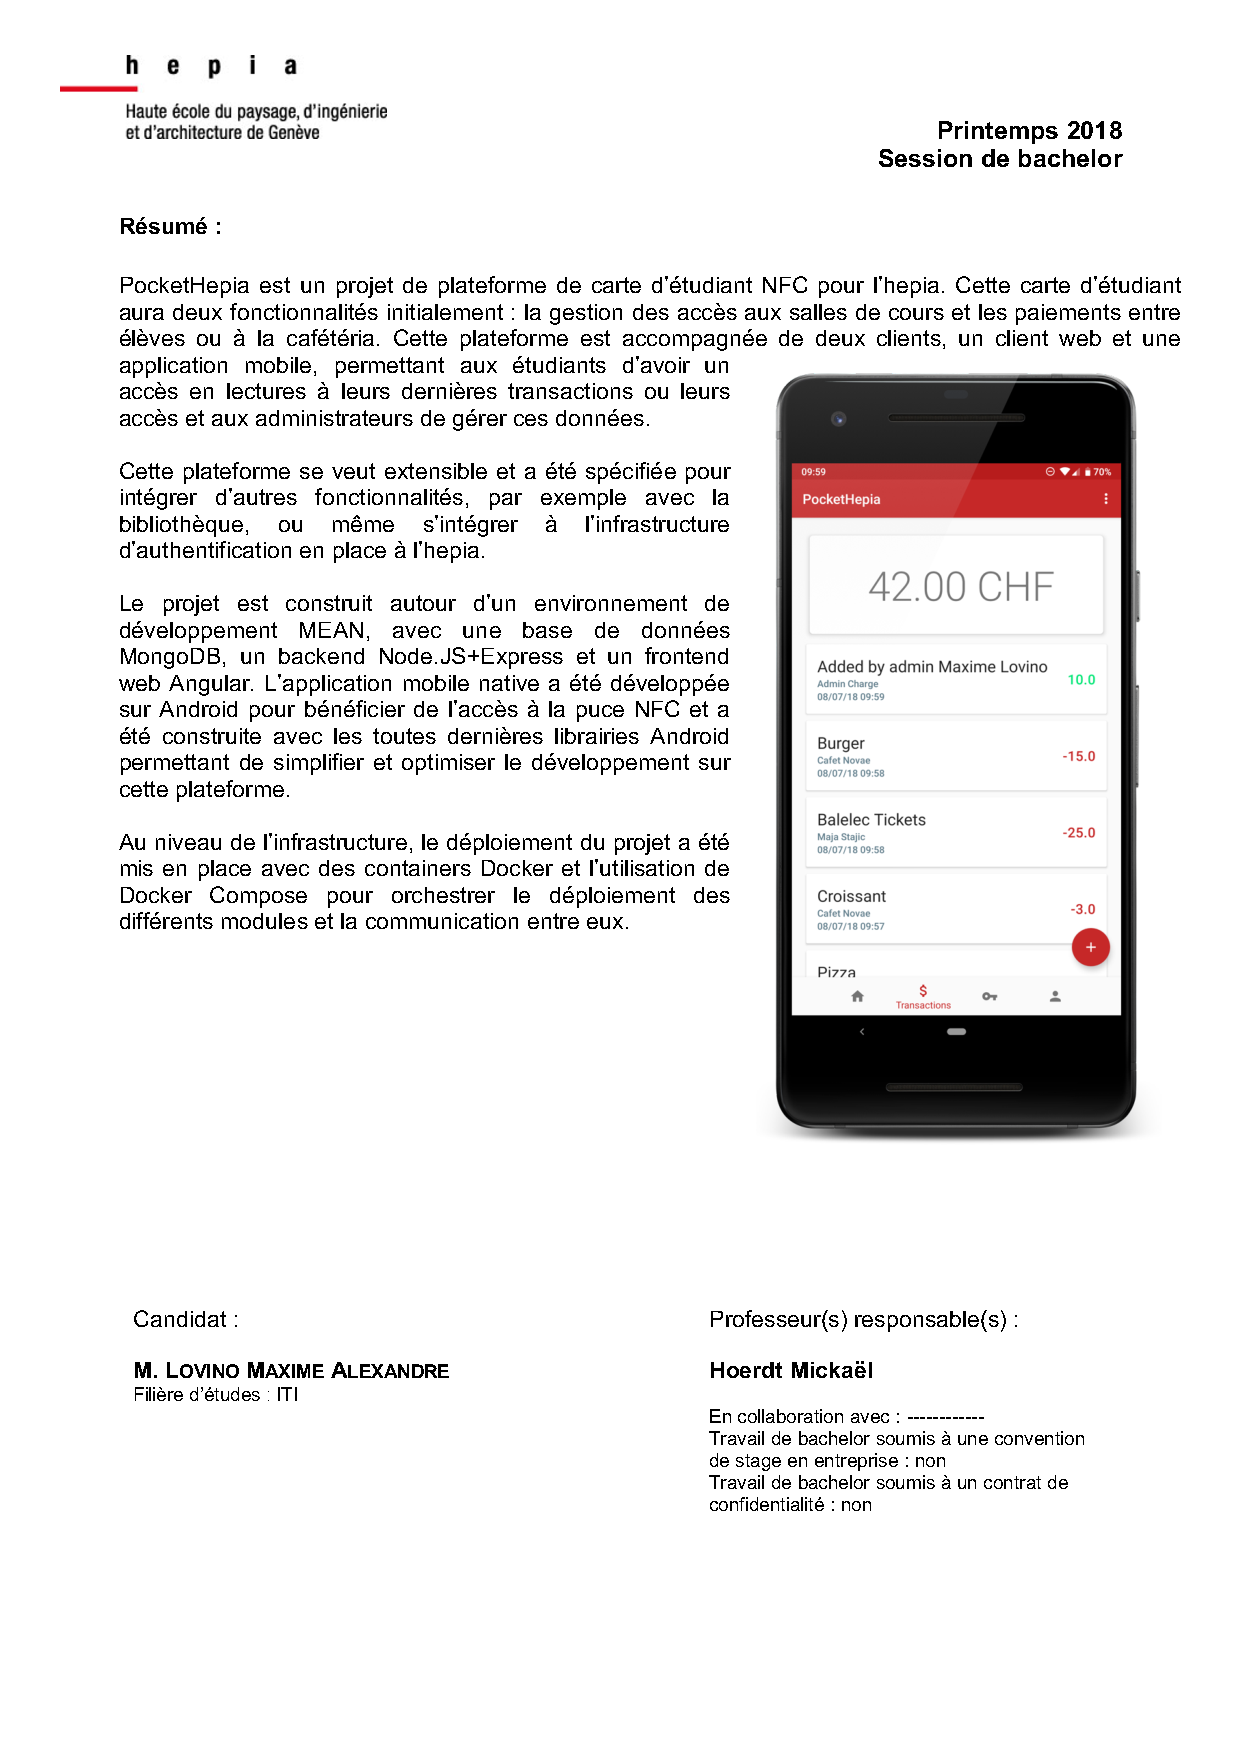
\includepdf[pages=1, pagecommand={}, scale=.9, offset=1cm 0]{ITI_Resume_PocketHepia}
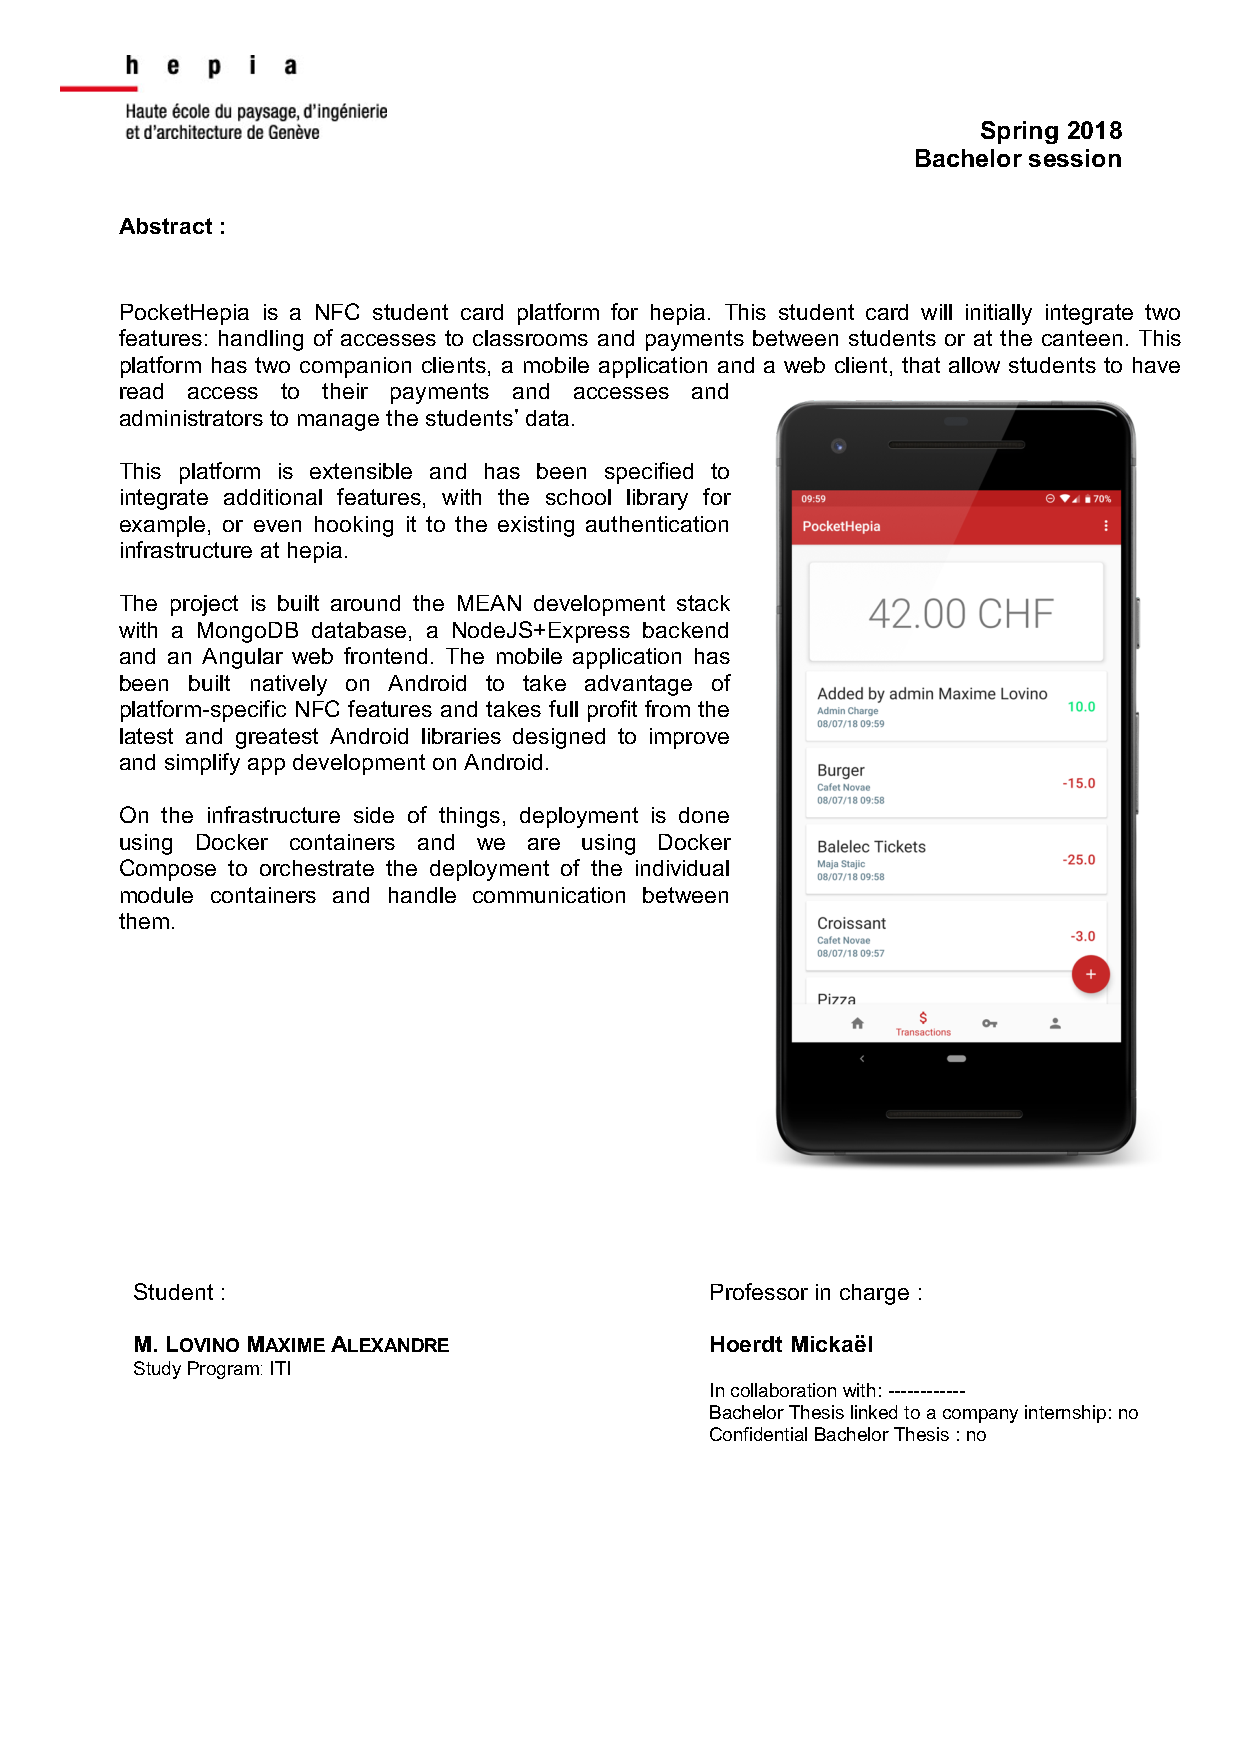
\includepdf[pages=1, pagecommand={}, scale=.9, offset=1cm 0]{ITI_Abstract_PocketHepia}
\tableofcontents
\listoffigures
\renewcommand\listoflistingscaption{Source code listings}
\listoflistings
\listoftables
\chapter*{Typographic conventions}
In this document, the following typographic conventions have been used:
\begin{itemize}
	\item All variables, classes or file names as well as function calls a are written using a monospace font, for example: \verb+User+
	\item All source code listings are written in blocks with syntax highlighting and a caption, for example:
	\bigbreak
	\begin{code}
		\begin{inlinets}
const username = 'Mickael';
console.log(`Hello world ${username}`);
		\end{inlinets}
		\caption*{This is the caption for the example source code}
	\end{code}
	\item Filesystem hierarchies are described using the \verb+dirtree+ package, for example:
\dirtree{%
.1 parent. 
.2 child\_1. 
.2 child\_2. 
.2 child\_3. 
}
\end{itemize}
\chapter*{Acknowledgements}
\printglossary[title=Terms and Definitions]
\newpage
\mainmatter
\pagestyle{hepia-fancy}
\pagenumbering{arabic}
\chapter{Introduction}
Since starting my studies at hepia almost three years ago after two years at \gls{epfl}, I've been shocked by the lack of commodities and study spaces for students. Some of this lack is due to the difference in scale between the two schools, one of them being composed of mainly three buildings in a constrained city environment and the other an almost-autonomous campus outside the city. But, actually, there isn't really a lack of space at hepia, but a lack of space that students can use to study. Most of the classrooms are locked when not in use by a teacher. When asking about why that is the case, I've been told that it was mainly for security concerns because of the equipment present inside the rooms. If the rooms stayed unlocked, there was no way of knowing who stole or broke something. I suggested the idea of giving access to select students to these classrooms to study and work on projects but it wasn't practical because copies of keys had to be made, the students had to make a money deposit to make sure that they didn't run away with the keys etc.\\ 

One solution would have been to use our student cards as an electronic door key to access the rooms. We could also enable other uses for the cards, such as using them as electronic wallets to simplify the payments at the canteen during lunch break. When I suggested the idea, people mostly laughed at me and said "[...] they're never going to do it, unless someone actually does it, presents it as a finished product and then they decide to use it." So, here I am, after 3 years studying at hepia and for my Bachelor Project I decided to work on this exact idea. A multi-function student card platform built on \gls{nfc} technology with accompanying mobile and web application for administrators to manage the platform and for students to monitor their usage statistics.


\section{NFC and NDEF}
We decided to build the student card around \gls{nfc} technology because it is practical to use for the end user and it provides everything we need to identify users with their card. Many personal identification solutions are built with \gls{nfc} for these same reasons.
\subsection{Introduction to NFC}
\gls{nfc} technology is a low range wireless communication technology based on electromagnetic induction. Its usages are widespread, ranging from access control to contactless credit card payments and public transportation tickets. The range of a \gls{nfc} communication is more or less 4cm. \gls{nfc} can be implemented in a physical chip on a card, in a discrete reader or in a smartphone. Most Android smartphones and all iPhones after 2016 have a \gls{nfc} chip. \\

There are three operating modes for \gls{nfc} devices. A device is considered a \emph{Full-\gls{nfc}} device if it can operate in the three modes, but most of the \gls{nfc} devices we interact with only support some of the modes:
\begin{itemize}
	\item The "card emulation" model, also called passive mode enables a device to be used as \gls{nfc} tag containing data similar to the ones present in physical \gls{nfc} cards. This mode is the only one available on devices with no power, for example credit cards. This mode is called passive because it uses power from the active \gls{nfc} reader to power it and enable access to its information. It can also be used on a smartphone to emulate a physical card. It is for example the mode used by mobile payments application such as Apple Pay and Google Pay. The \gls{nfc} reader simply detects a standard \gls{nfc} card, without knowing that is in fact emulated by a smartphone.
	\item The reader mode, also called active mode. This mode allows reading \gls{nfc} tags data with a smartphone or a specific reader, for example in an electronic doorknob or a metro station gate.
	\item The peer-to-peer mode is used by two smartphones to exchange information between them. This mode is used on Android by the Android Beam service which allows to send pictures or other data between two Android devices by placing them back to back. In this case, the \gls{nfc} peer-to-peer mode is used to initiate the connection and pair the device and then the data transfer is carried over Bluetooth or Wi-Fi Direct.
\end{itemize}
\begin{figure}[H]
\begin{center}
	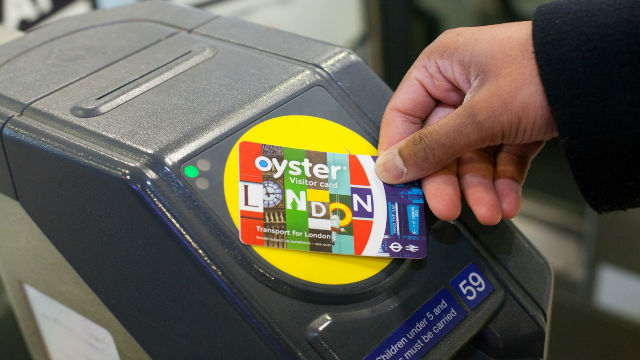
\includegraphics[width=.6\textwidth]{assets/oyster_reader.jpg}
	\caption[NFC reader and Oyster Card]{A \gls{nfc} card reader on the London Underground (active mode) and a Oyster Transport Card (passive mode) \cite{img:oyster}}
\end{center}
\end{figure}

\subsection{NDEF Format}
The \gls{ndef} format is a standardised format used to encode data on \gls{nfc} tags. By using a standard format, it allows for easier exchange of information between \gls{nfc} devices. A \gls{ndef} message is composed of \gls{ndef} records. Each of these records contains metadata that provides information to help decode the data payload contained in the message.\\

The format of a \gls{ndef} record is the following\cite{nfc:ndef:adafruit:article}:
\begin{verbatim}
	Bit 7     6       5       4       3       2       1       0
------  ------  ------  ------  ------  ------  ------  ------ 
[ MB ]  [ ME ]  [ CF ]  [ SR ]  [ IL ]  [        TNF         ]  

[                         TYPE LENGTH                        ]

[                       PAYLOAD LENGTH                       ]

[                          ID LENGTH                         ]

[                         RECORD TYPE                        ]

[                              ID                            ]

[                           PAYLOAD                          ]
\end{verbatim}
The first byte form the header of the \gls{ndef} record, the fields composed the header are:
\begin{itemize}
	\item The \verb+TNF+ (Type Name Format) is a 3 bits value used to identify the record type. The most common are "Empty record" and "Well-Known-Record" to define a record for which the data type is defined by a RTD (Record Type Definition) in the \gls{ndef} format, for example plain text or URI.
	\item The \verb+IL+ (ID LENGTH field) is a boolean 1 bit value to tell if the \verb+ID LENGTH+ field is present or not in the record.
	\item The \verb+SR+ (Short Record Bit) is a boolean 1 bit value to tell if the \verb+PAYLOAD LENGTH+ has a size of 1 byte or less.
	\item The \verb+CF+ (Chunk flag) is a boolean 1 bit value to tell if the record is the first part or a chunk of a bigger record. The value will be 0 if it is the only part or the last chunk of a record.
	\item The \verb+ME+ (Message End) is a boolean 1 bit value to indicate that the record is the last of the \gls{ndef} message.
	\item The \verb+MB+ (Message Begin) is a boolean 1 bit value to indicate that the record is the first of the \gls{ndef} message.
\end{itemize}
\subsubsection{Text payload}
To give an example of a data payload contained in a \gls{ndef} record, we are going to take a closer look at a plain text payload.

The text payload format is defined like this\cite{nfc:ndef:doc:text_record} :
\begin{verbatim}
	Bit 7     6       5       4       3       2       1       0
------  ------  ------  ------  ------  ------  ------  ------ 
[ ENC]  [RFU ]  [                IANA LENGTH                 ]  

[                       IANA LANGUAGE CODE                   ]

[                           TEXT                             ]
\end{verbatim}
The first byte is called \verb+Status Byte+ and contains \verb+ENC+ which stores the value of the encoding used in the payload (0 for UTF-8, 1 for UTF-16) and \verb+IANA LENGTH+ which stores the length of the \verb+IANA LANGUAGE CODE+ field found afterwards. The \verb+RFU+ bit is always set to 0. In the \verb+IANA LANGUAGE CODE+ is stored the ISO/IANA language code specifying the language of the text stored in the payload as defined in RFC 3066\cite{rfc:language}, for example "en-US" for American English. The encoding of the language code is always ASCII. Finally we have the text whose length is the length of the payload minus 1 byte and the length of the language code field. The text can be decoded using the encoding specified in \verb+ENC+

\section{Project inspiration - Camipro EPFL}
\subsection{The card and the official core platform}
The inspiration for this project mainly comes from my experience studying at \gls{epfl}. The \gls{epfl} student card, named Camipro\cite{camipro:homepage}, contains a \gls{rfid} chip that allows to perform various tasks that simplify student life on campus. The use cases for the Camipro card are the following:
\begin{itemize}
    \item Electronic wallet to pay at every canteen on campus as well as select third-party retailers (for example the Migros shop present on campus)
    \item Access key to unlock doors and buildings
    \item Card to collect documents sent to the centralised printing pool system at any printer on campus
    \item Rent public bicycles\footnote{All students have access to a free Publibike account on their card \url{https://www.publibike.ch/en/publibike/}} on campus and in the Lausanne area
    \item Rent cars by linking a Mobility\footnote{\url{https://www.mobility.ch/en/}} subscription to the card
    \item Borrow books at the library
    \item Use electric car chargers on campus
    \item Turn on booked electrical barbecues present on campus\footnote{The service PolyGrill allows students to book free barbecues on campus and access them with their camipro \url{https://camipro.epfl.ch/cms/site/camipro/lang/en/polygrill_electric_barbecues}}
\end{itemize}

An accompanying web platform called MyCamipro was built as part of the Camipro launch to manage and activate the different services on the card as well as see the recent transactions and the rooms we were given access to.

\begin{figure}[H]
\begin{center}
	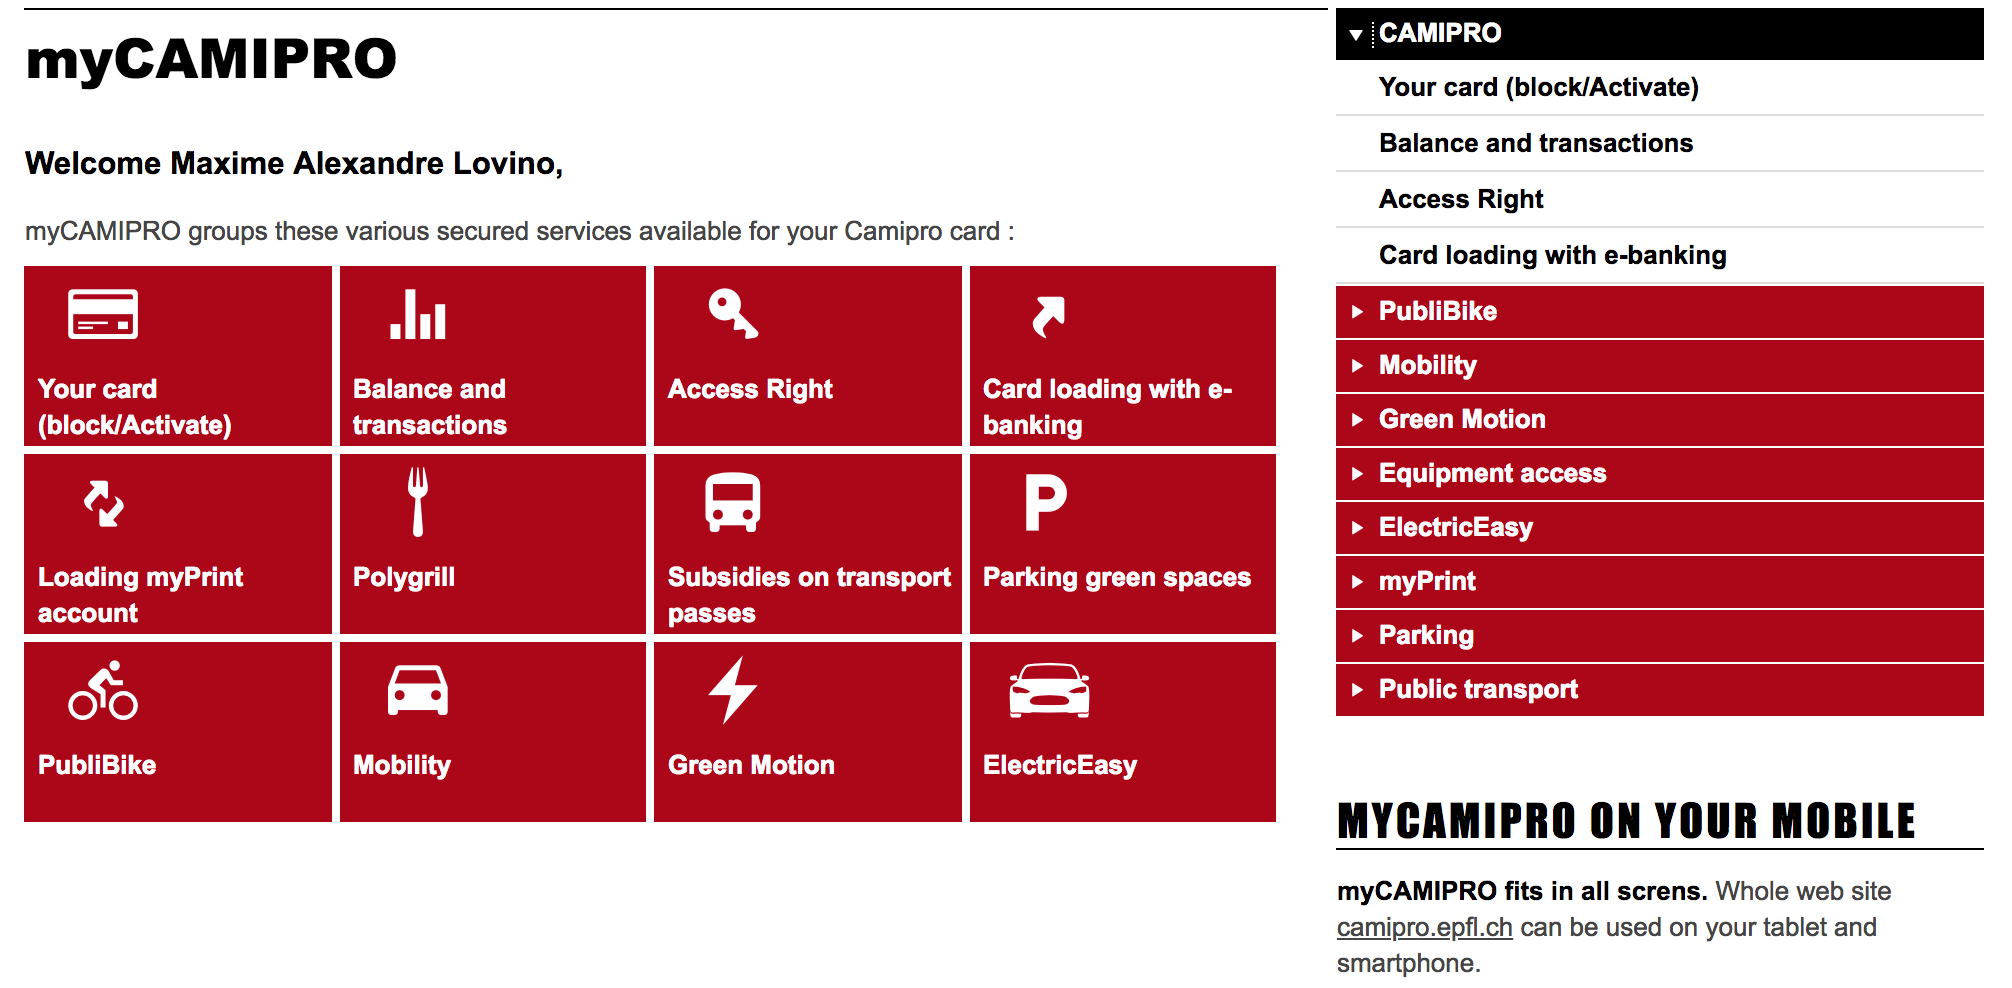
\includegraphics[width=.6\textwidth]{assets/camipro_website.png}
	\caption{Screenshot of the MyCamipro website}
\end{center}
\end{figure}

\subsection{PocketCampus}
With the increased usage of smartphones by students, in 2010 a team of 20 computer science students decided to build the PocketCampus application as part of a software engineering class. They continued working on the project after the academic project was finished and it became the official \gls{epfl} application in 2013. \cite{camipro:creation}. \\

Initially you could mainly see the balance of your Camipro card on the app, but version after version, the development team added new integration in the app by collaborating with different services at \gls{epfl}.
These functions include:
\begin{itemize}
    \item Accessing the menus of all canteens on campus
    \item Searching through the whole \gls{epfl} directory
    \item Having access to IS-Academia data to see course schedule and grades
    \item Printing from your smartphone on the \gls{epfl} print system
    \item Accessing Lausanne public transportation itineraries
    \item Accessing Moodle documents
\end{itemize}

After having integrated every requested features, the team launched a beta web version of PocketCampus for \gls{epfl} in June 2018. They also started diversifying their business by working on PocketCampus as a platform that can be integrated in other companies and stopped working exclusively with \gls{epfl}. They announced plans on partnering with Lausanne University (UNIL) to integrate their platform there.

\begin{figure}[H]
\begin{center}
	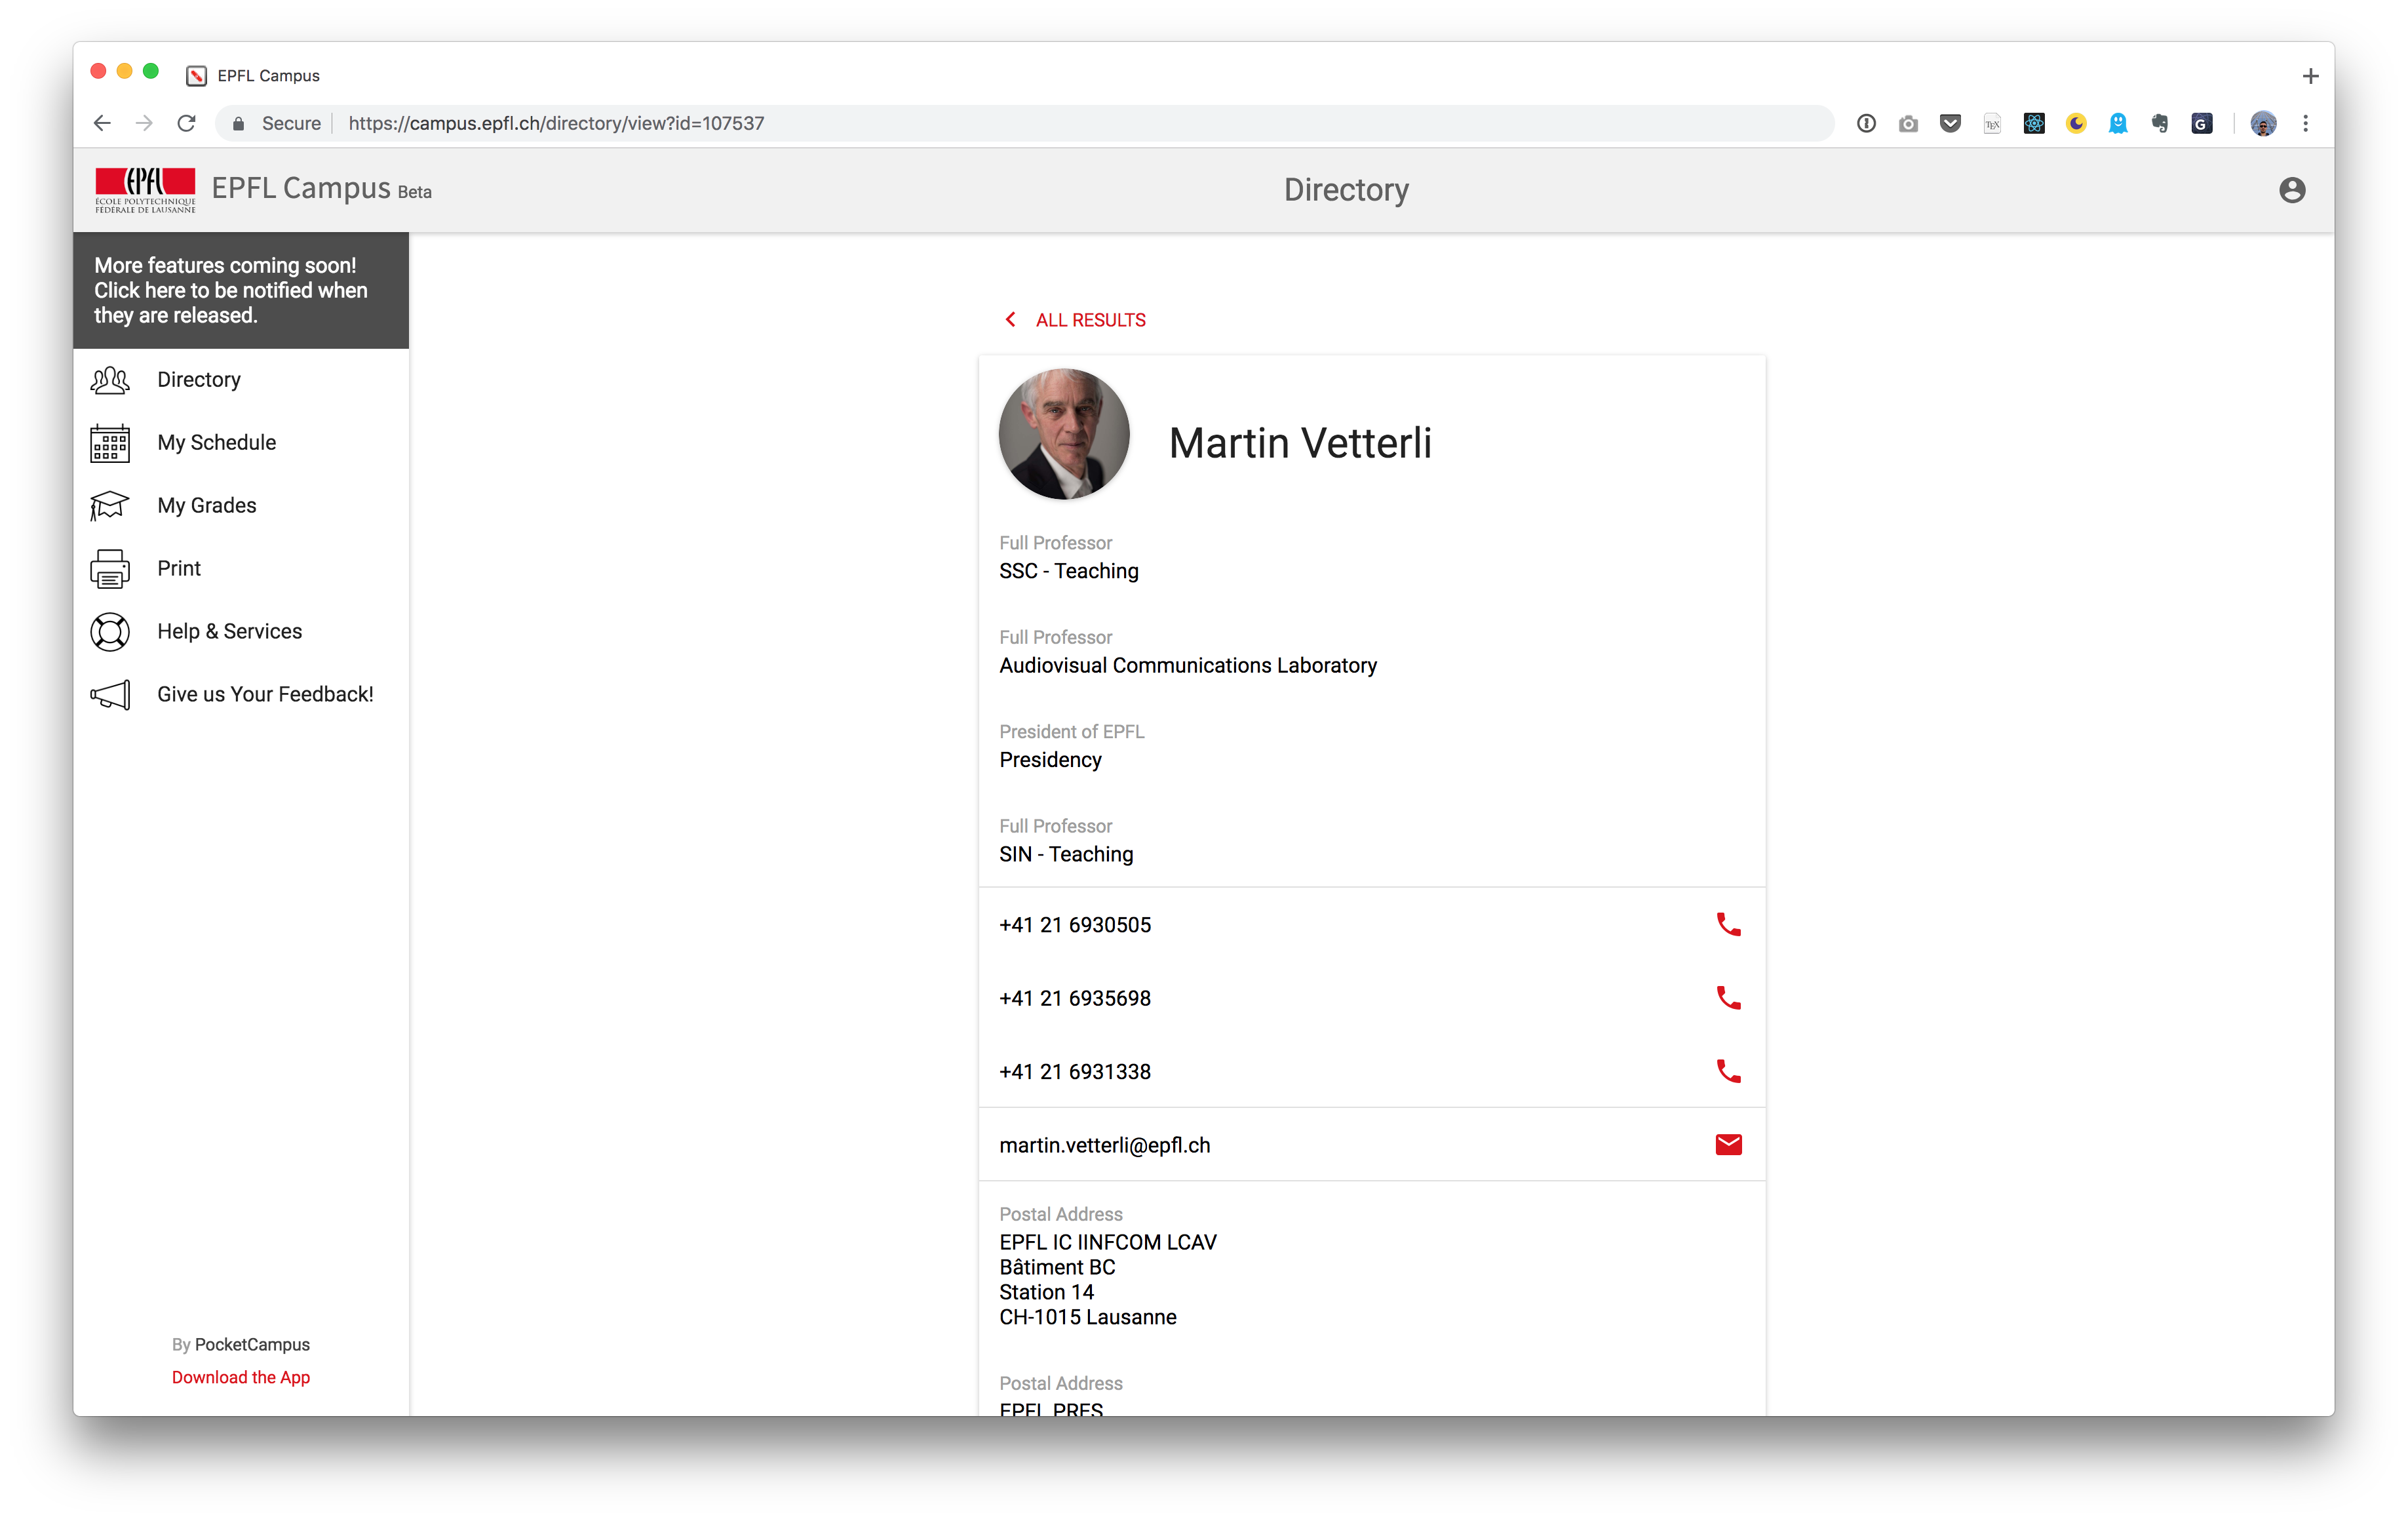
\includegraphics[width=.8\textwidth]{assets/web_pocketcampus.png}
	\caption{Screenshot of the web version of PocketCampus}
\end{center}
\end{figure}


\begin{figure}[H]
\begin{center}
	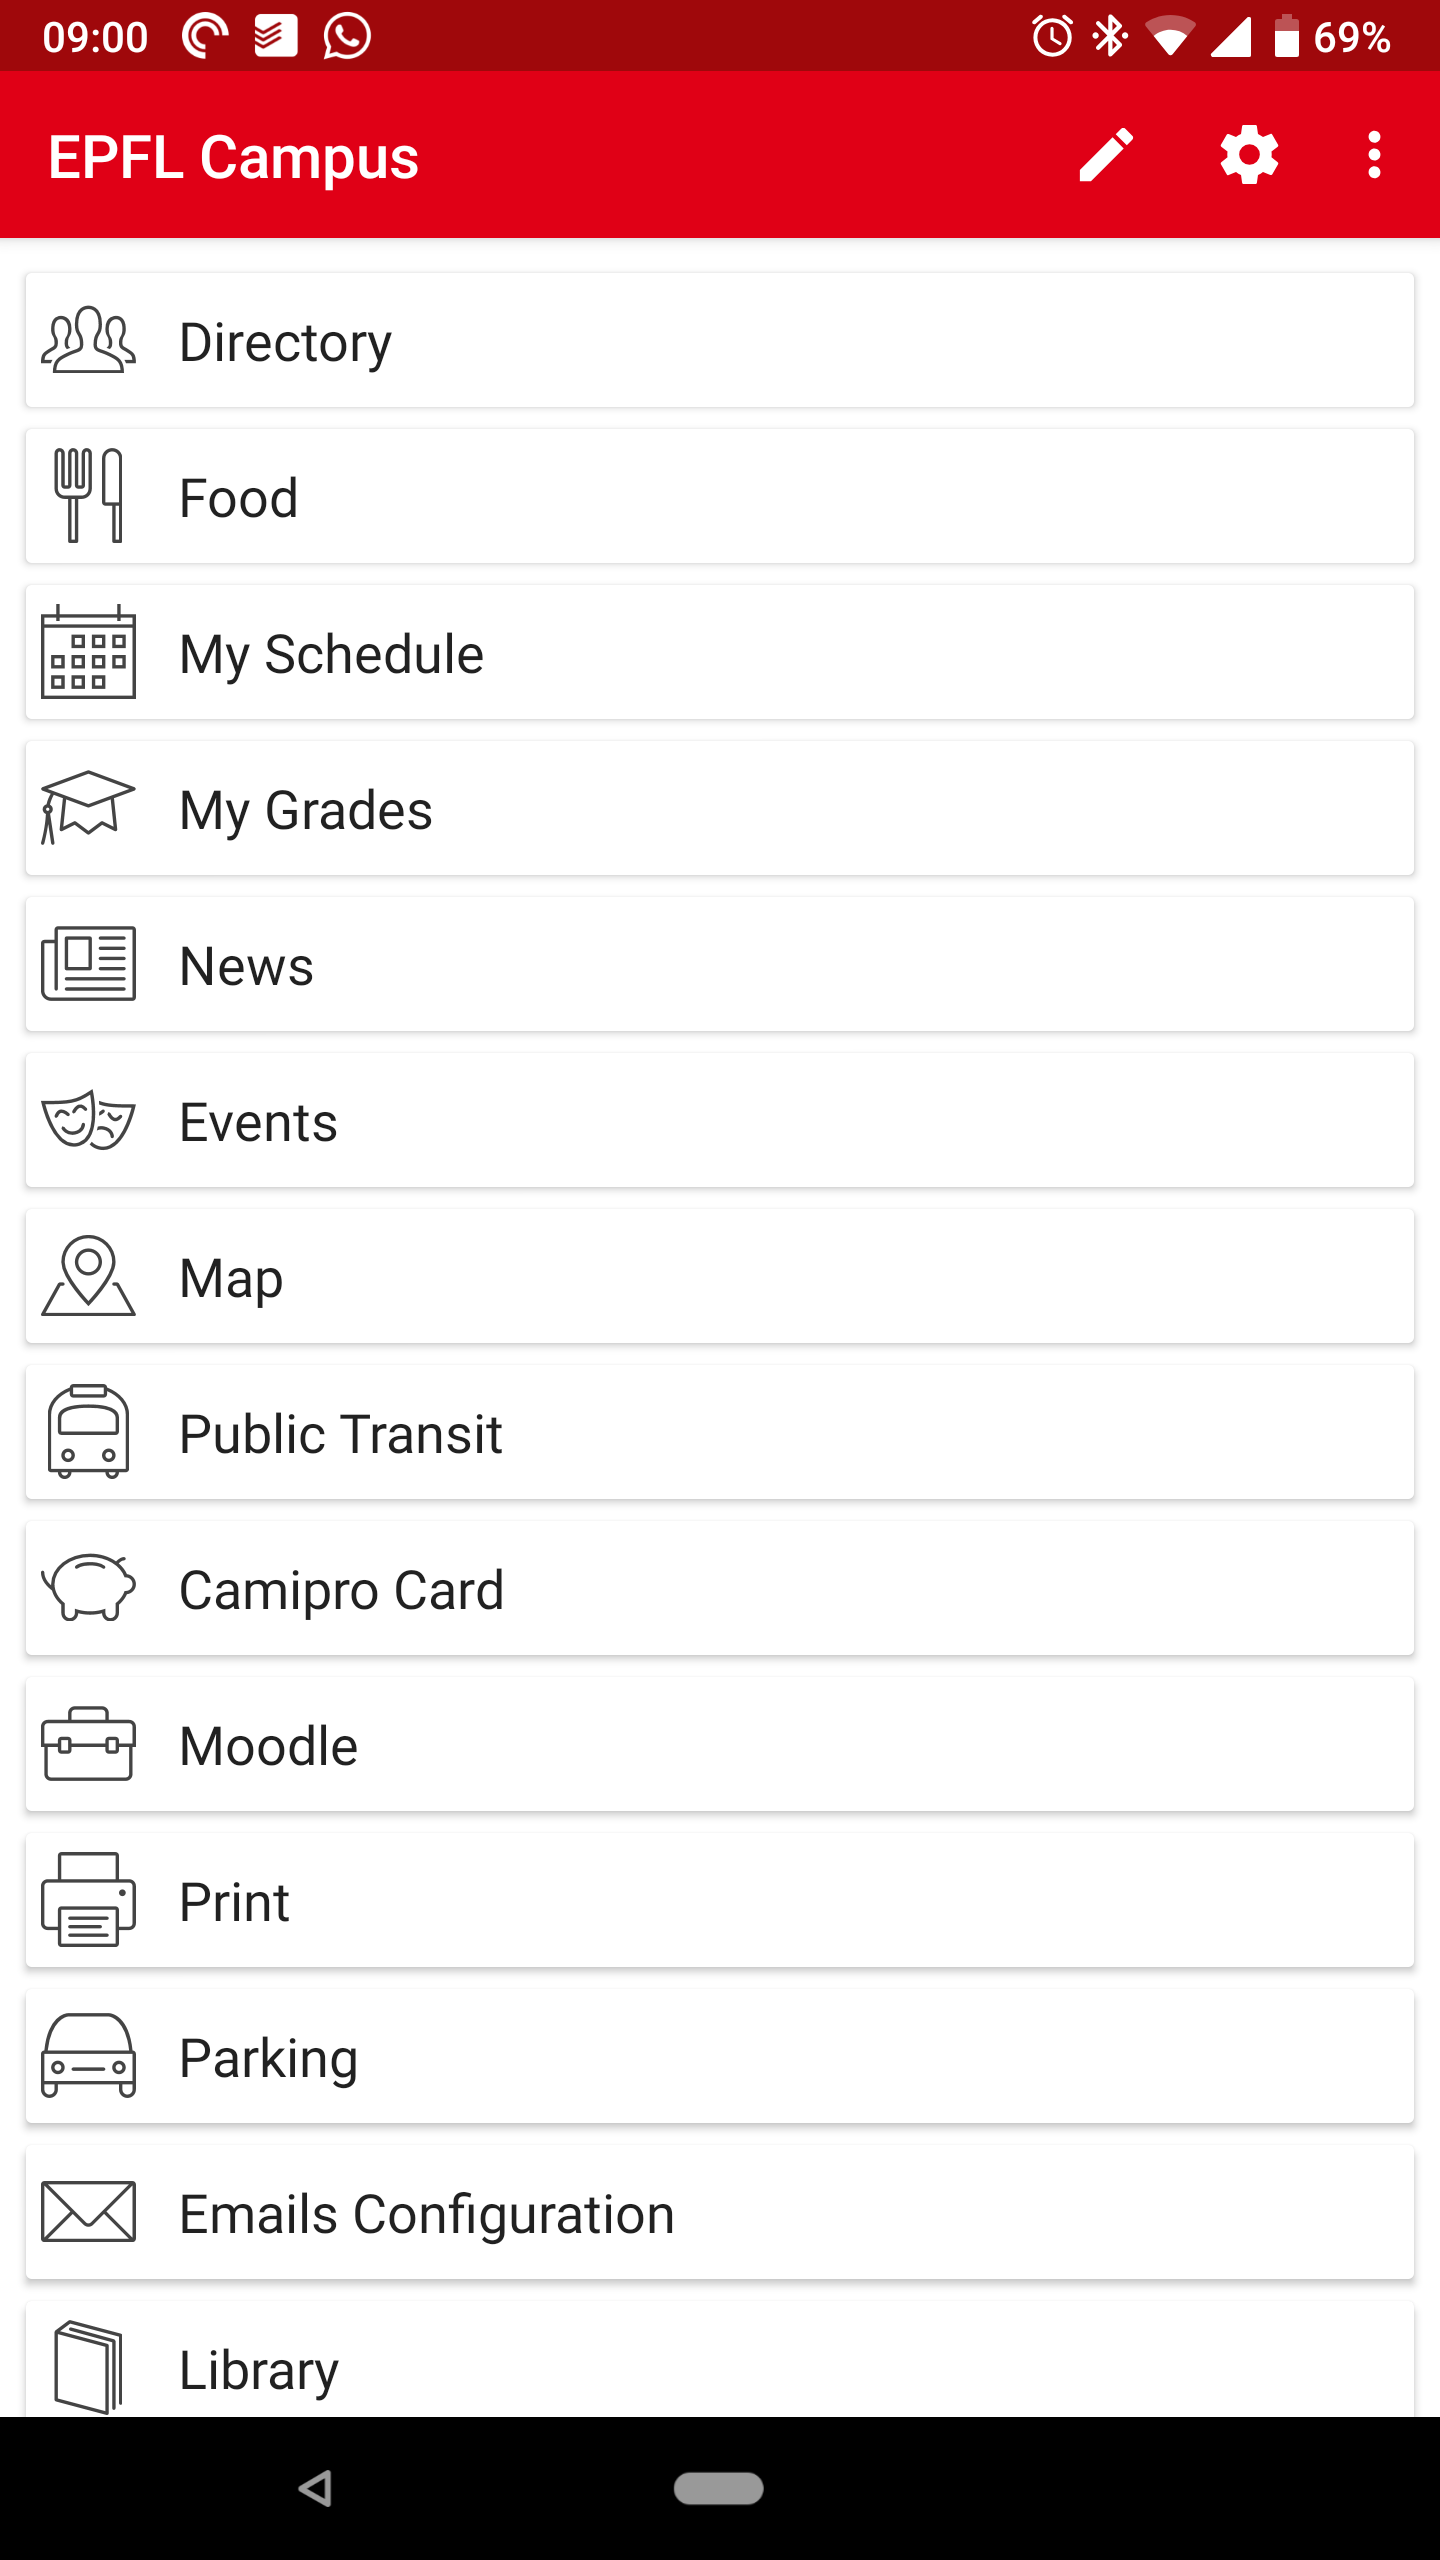
\includegraphics[width=.5\textwidth]{assets/pocketcampus_mobile.png}
	\caption{PocketCampus Android application}
\end{center}
\end{figure}

\chapter{The project}
The project is called PocketHepia, reminiscent of the name of the project at \gls{epfl} and will consist of the two parts of the \gls{epfl} project presented earlier: the student card platform, as well as the applicative platform to access information.\\


The idea of this project is not to build as many features as the \gls{epfl} platform due to the time constraints inherent to the Bachelor Project, but rather to focus on some key aspects of the card at first, namely payments, access control and library. We are also building features on the payment side that are not available on the \gls{epfl} platform, for example the ability to send money between users. The project of course will be extensible with other features outside the scope of the Bachelor Project. \\

In this chapter, we will present the main features, roles and user stories for the project as specified at the beginning of this one. All of these are part of the project, but not necessarily part of the Bachelor Project. The idea was to specify the entire project and to start implementing a subset of the functionality for the academic project and continue working on the rest as well as new features outside this scope. Mainly we wanted to remain independent of other school services and infrastructure because of the associated time it would take to get permissions and setup integrations, as well as restrictions to development environments to secure access to these services. For each element of this chapter, we will specify whether it is going to be implemented as part of the Bachelor Project.\\

The project is composed of three main components:
\begin{itemize}
    \item The physical student card
    \item An administration component
    \item An user facing component
\end{itemize}

A mobile application and a web application will be developed and both will offer the same user facing features as well as specific administrative features relevant to each application.

\section{Features of the app}
As stated before, we decided to limit the project to the three most important features in our opinion and, out of these, two are going to be implemented as part of the bachelor project.

\subsection{Payments}

The first feature is the electronic wallet functionality. We decided to start with this one because it would be bring the most benefits to the students and would not need specific hardware or collaboration with any school service. Every user has an electronic wallet linked to its account on the platform and can then send money to any other user by choosing the amount to send and tapping the user's card on his phone. Users can be assigned a specific role (see section \ref{roles_section}) to allow them to receive money directly from a card.\\

There will be two main ways to add money to an user wallet. Either the user can give cash money to a person with administrative role that will then add money to the user's balance. Or the user will be able to add money to its account by using its credit card on the web application.\footnote{At the moment, the project is still in the development phase so no bank accounts have been linked to this project and you will be able to recharge your account only using a specific test credit card generated for development purposes}

\subsection{Accesses}

To continue, the second element of the project is the handling of access control through the platform. This was the original pain point we noticed at hepia with the lack of an easy way to handle accesses to the available classrooms. We will be able to create different areas to group rooms inside them. For example, an area could be an entire floor or labs for a specific section of hepia.\\

As far as giving access to users, we can give access to a room from a given date and specify if needed an end date for the access. For example, we can setup access for a user until the end of the current semester. We also decided to introduce an optional time range during the day during which the given access is active, so we can for example allow a student to enter a room only between 8am and 7pm. \\

We also specified the ability to delegate the administration of an area to a user, so that access to rooms can be handled at a department or section level in the school for example (see section \ref{roles_section}). This feature is planned but will not be implemented as part of the Bachelor Project.

\subsection{Library books}
\label{books_feature}
Finally, the last feature of the project would be an integration with the library to be able to use the card as a library card. Our approach at first was to think about creating the book loans on our platform with the ISBN to identify the book and integrate with the \gls{rest} \gls{api} built for BibApp\cite{playstore:bibapp} but it wouldn't have been very effective because the library already handles the loans through the NEBIS platform.\\

The correct way to handle this would be to link the library NEBIS identifier for every user with their account on our platform and then ask NEBIS for \gls{api} Access to their platform to retrieve book loans for all users and display them on the mobile and web application. This would also benefit people working at the library as they would not need to change their current workflow to accommodate.\\

We don't have the time during the bachelor project to start a discussion with NEBIS to get access to the required information so this feature will have to be implemented later on.
\section{Roles}
\label{roles_section}
We defined a set of roles for the users on the platform. First, every member of the platform is a simple user. This means that the person has an account on the platform, can login to the web and android application and has read access to its payments, its accesses and its other information and can send money to other users.\\

Then, there is the admin role that can be added to an user. This role enables the creation of users, attribution of roles, the consultation of administrative logs as well as the creation of access components (rooms, readers) and the attribution of accesses to users.\\

While these two roles would have been enough to handle all our features. We decided to specify roles specific to different components of the platform.\\

One of these roles is the "Accept payments" role. This is specific to a canteen or a shop that wants to handle payments using the student card. While every user can send money to another user from the mobile app by tapping the other user's card, this isn't very practical for a canteen or a shop where the transactions should go the other way around. So the shop creates the payment and taps the user's card to take money from it. At first, we wanted this feature to be available to everyone but we thought about security concerns with this solution because a student could create a payment from the app and start tapping his phone on lost cards or even on people's pocket and if the card was detected it would "steal" their money. So by enabling this feature as a role, we could only allow trusted people, such as canteen's owners to receive payments in that way. \\

Furthermore, due to the introduction of GDPR\footnote{GDPR stands for \emph{General Data Protection Regulation} and is a new regulation implemented as of May 25 2018 in the European Union and Switzerland to improve data protection and privacy\cite{gdpr}} recently, we created a specific role called "Auditor" to access sensitive logs concerning all users, mainly access logs and transaction history. Only a user with this role can view all transactions between users and access logs for every room.\\

Then, there are two roles that will not be implemented as part of the Bachelor project, the "Can invite" and "Area admin" role. The first is to allow specific users to create temporary accounts without needing to contact an administrator. A use case for this would be a teacher creating a temporary account for a visiting colleague from another school. The "Area admin" role consists of delegating the administration of the accesses for an area to an user. Similar to the concept of DNS zones delegation, an administrator could for example give this role to the ITI section dean to allow him to give access to the rooms present on his floor.\\

Finally, the last role is the "Librarian" role that as its name implies is attributed to users working for the library. This role enables the creation of books loans at the library for users. As stated in section \ref{books_feature}, this role will certainly be removed completely because there is already a system in place to handle book loans at the library.

\section{The models}
%%TODO should we talk about books
%%TODO should we add not implement models to the schema, for example access requests
\begin{figure}[H]
\begin{center}
	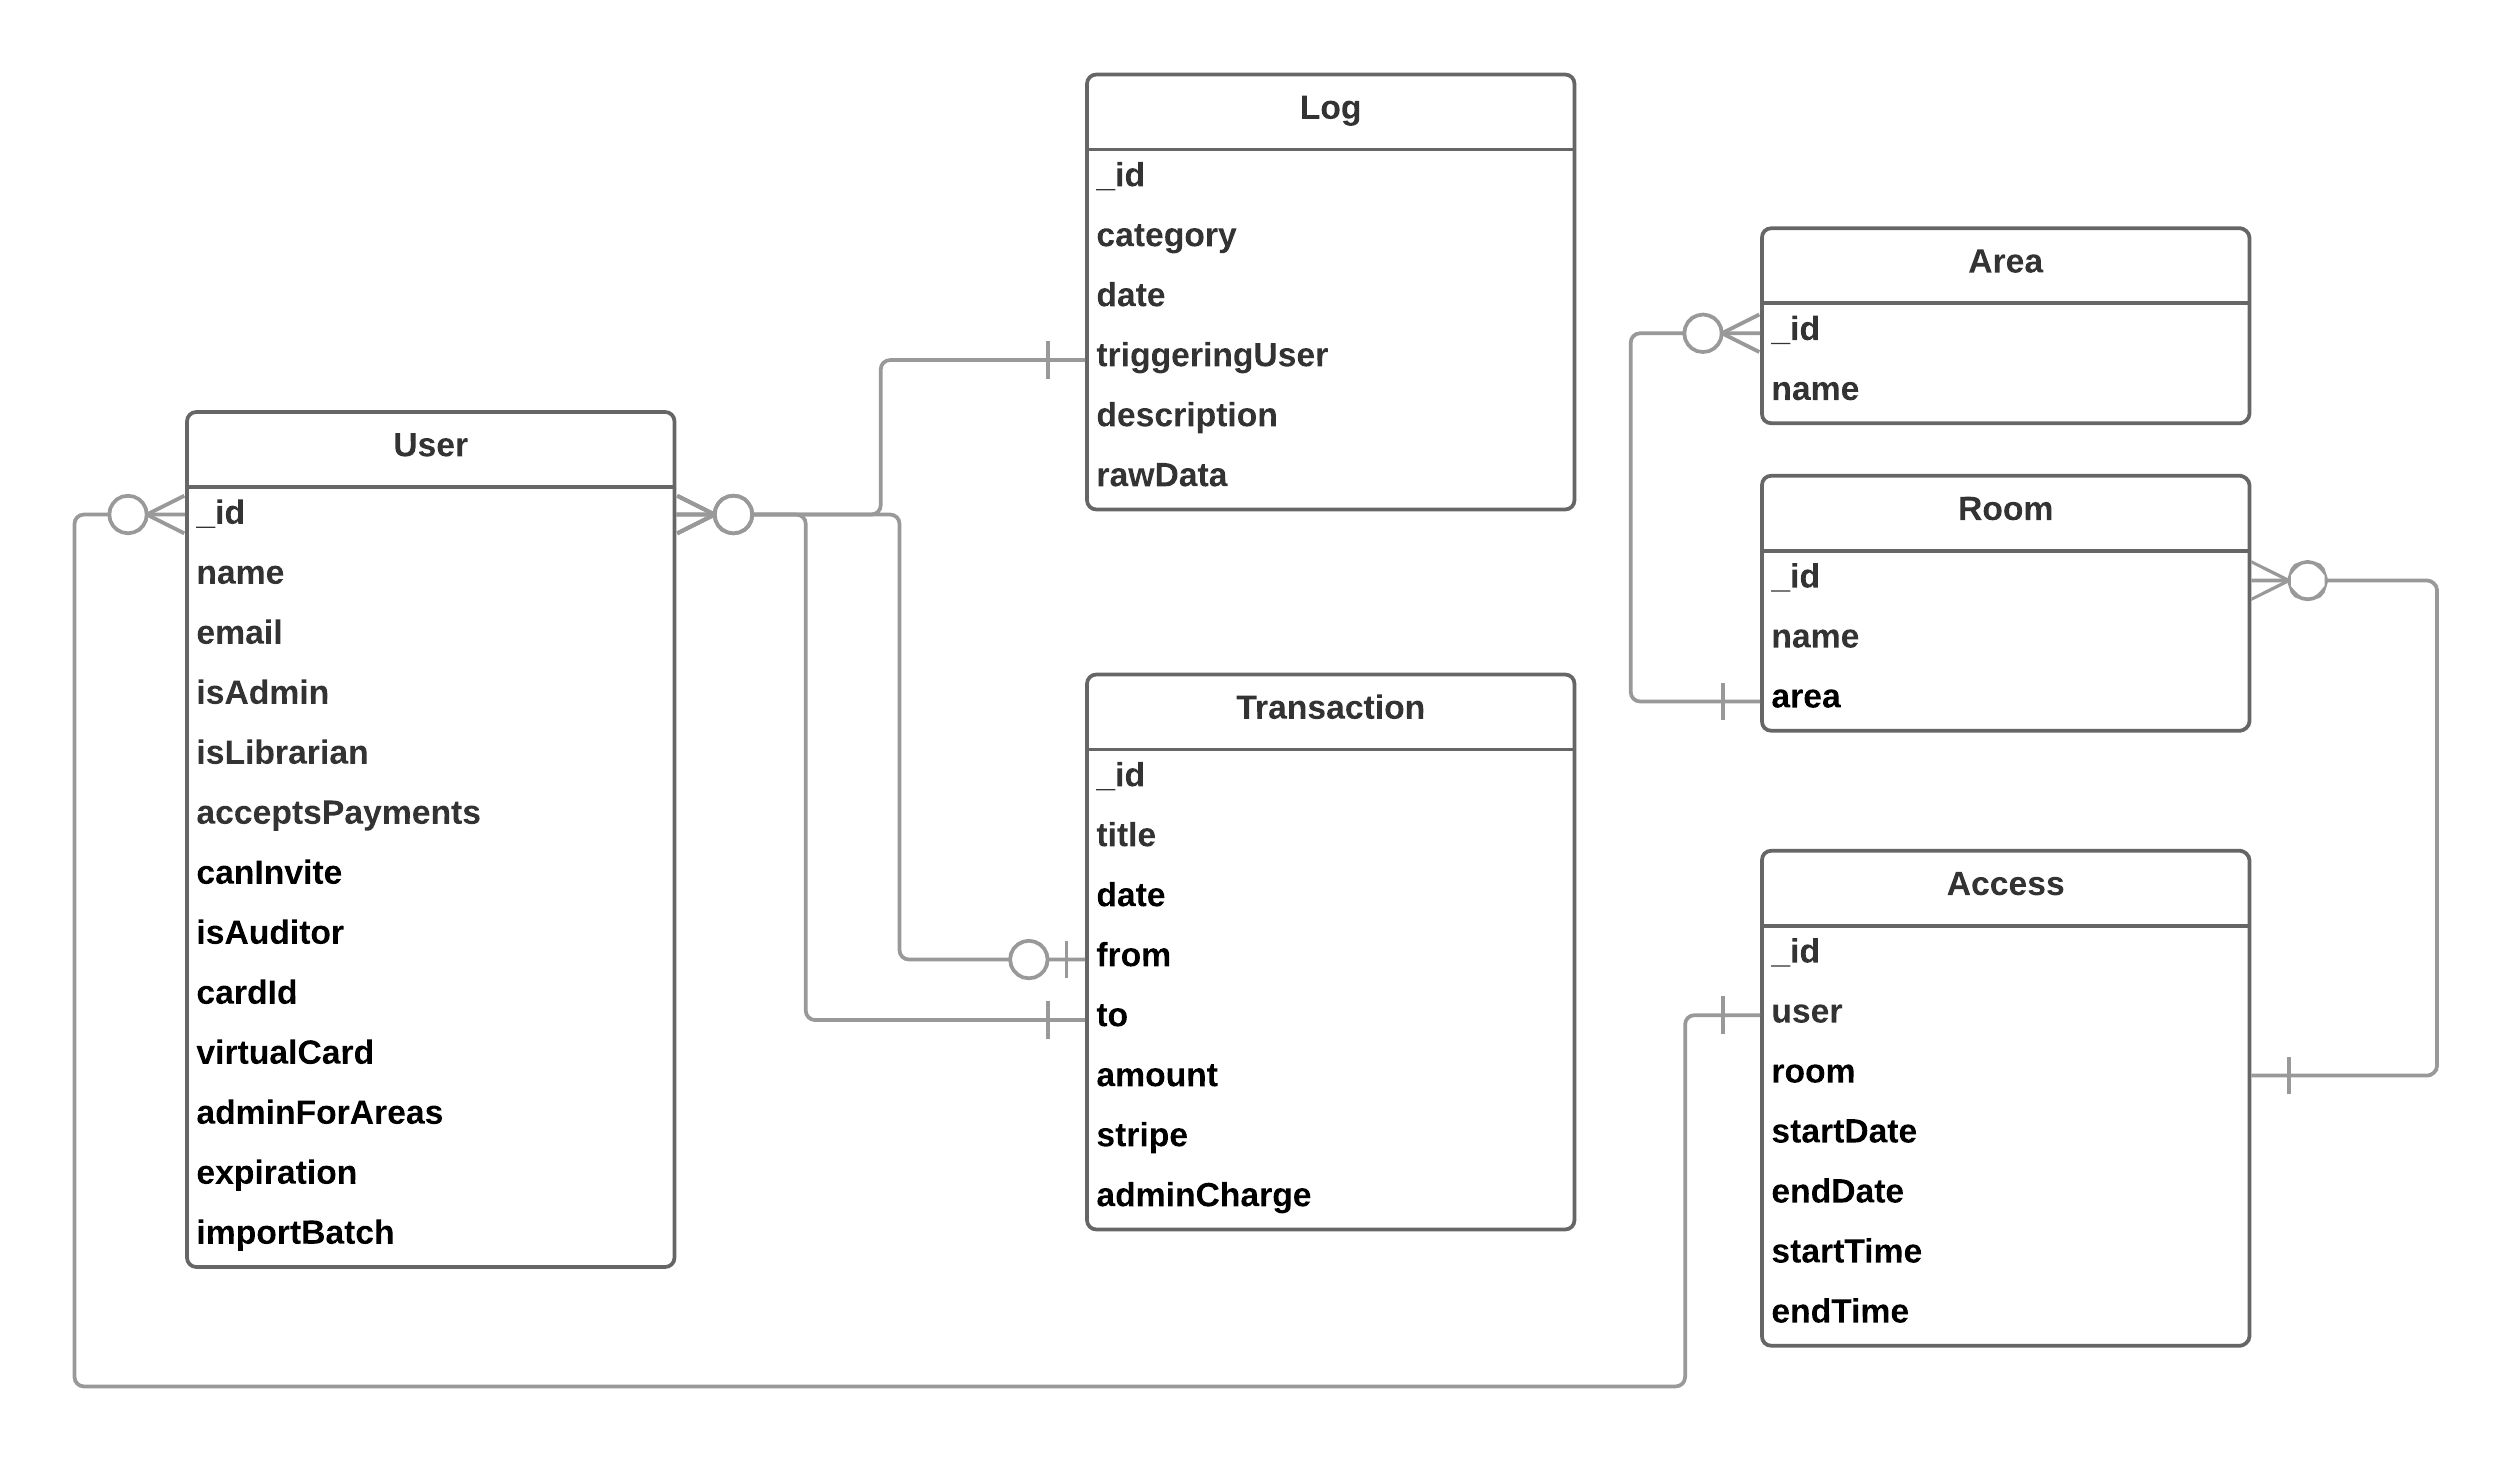
\includegraphics[width=\textwidth]{assets/models_relation}
	\caption{Entity Relationship Diagram of the models}
\end{center}
\end{figure}
\subsection{User Accounts}
\begin{figure}[H]
\begin{center}
	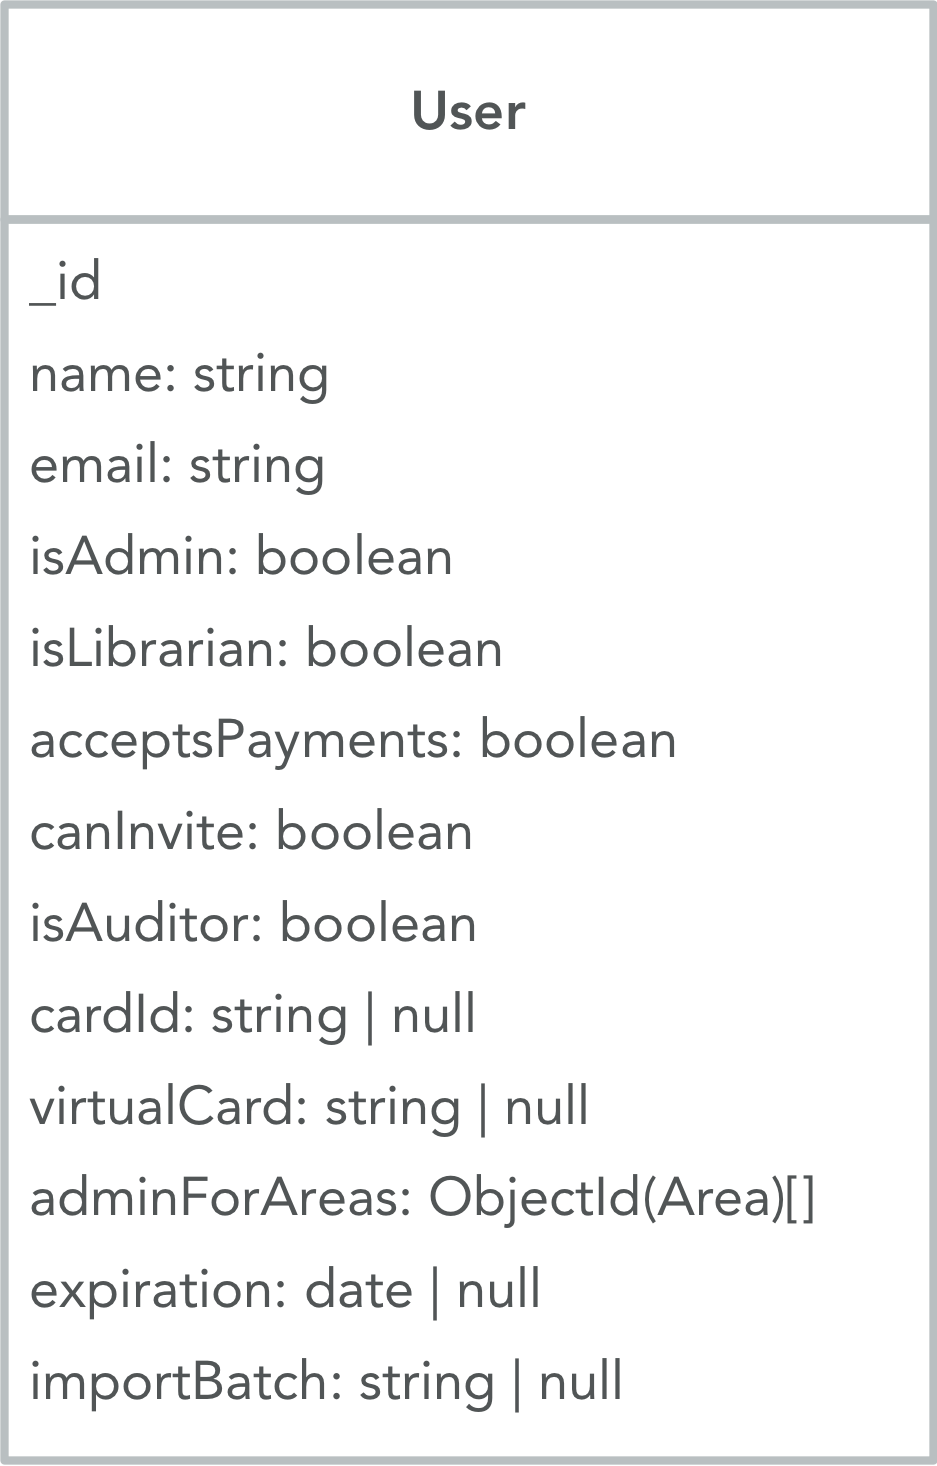
\includegraphics[width=.4\textwidth]{assets/user_model}
	\caption{User Model}
\end{center}
\end{figure}

The first of our models is the User. A user collection is created to store all users on the platform. Users are identified by their email address and will login with their email and password, their full name is also stored. The authentication specific fields will be added to the model by Passport.JS (see section \ref{technological choices}). A boolean field is also stored for each permission.\\

The expiration date, the virtual card and the delegation of admin zones are not implemented as part of this bachelor project. \\

Finally, the \verb+importBatch+ is set if the user is imported with a CSV file so that we can group all users imported together and undo the import if necessary.
\subsubsection{Integration with existing AAI user accounts}
If this project is put in production at hepia, we will have to only change this model to integrate it with an existing authentication service, such as AAI or with a directory LDAP service.\\

In that case, we would remove information already present in the authentication service such as name and email and just store the unique identifier from the authentication service in our model. This model would act as an augmented database on top of the existing service. We would then forward all login/password authentication request to the authentication service and would create the entry for the user in our database after the first login.\\

This is inspired by the way Nextcloud\footnote{\url{https://nextcloud.com/}} for example stores user accounts that are linked to a directory service, for example an Active Directory. It stores the full Distinguished Name from the directory service as the unique identifier for the account to link the local account to the directory account.\\

While we could have asked Switch-AAI to integrate AAI authentication in our application, the time constraints of the project were too tight to launch a discussion and we wanted to stay independent of other services in this phase to avoid being slowed down by for example needing to run our servers on the hepia network exclusively to access the directory.
\subsection{Payments}
\begin{figure}[H]
\begin{center}
	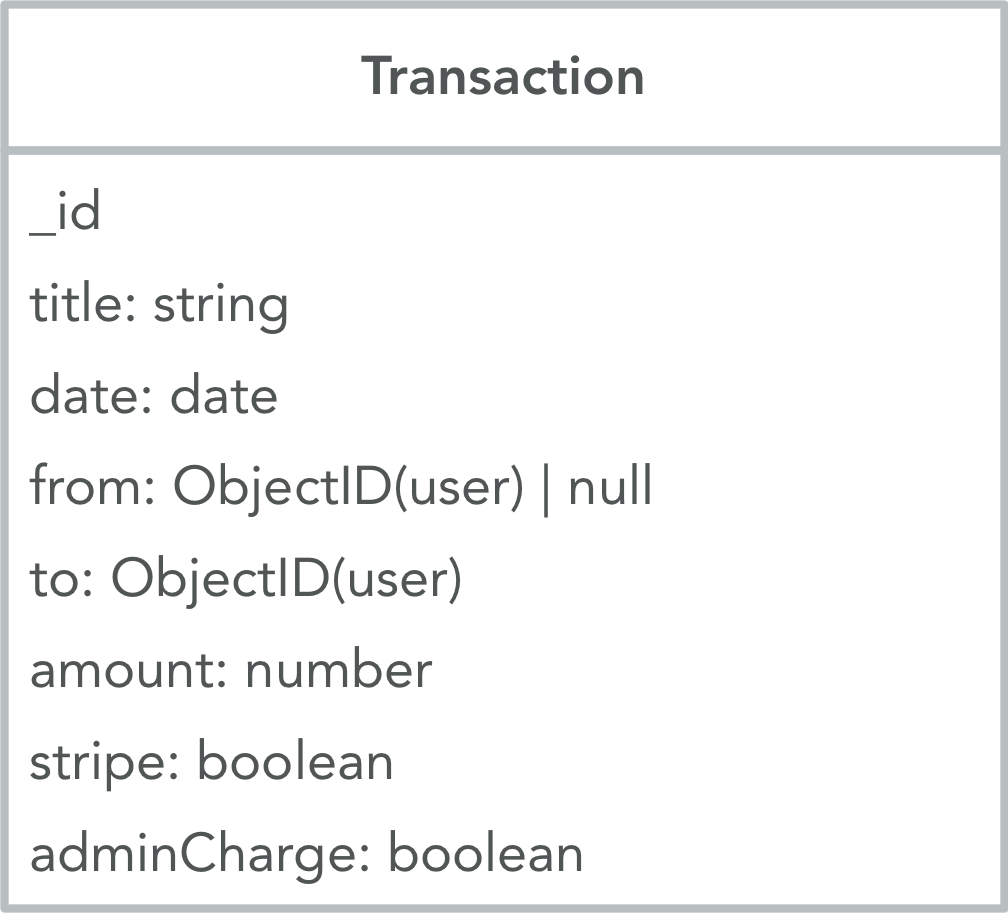
\includegraphics[width=.4\textwidth]{assets/transaction_model}
	\caption{Transaction Model}
\end{center}
\end{figure}
To handle payments, we defined a Transaction model that represents a money transaction. We store the id of the \verb+to+ and \verb+from+ users instead of embedding the users document inside the transaction in order to avoid using too much space in the database. The number of transactions can grow very high and it is a waste of space to store two full user documents in each transaction\footnote{For more on that, see section \ref{mongo_references} on Mongo References}. Finally, we handle the two type of recharges for the user account by setting the \verb+from+ user to \verb+null+ because the money does not come from any user account and set the corresponding \verb+stripe+ or \verb+adminCharge+ field to true. \\

The balance of a user is calculated from the list of transactions in which the user takes part. It is calculated as the sum of the transactions in which the user is the beneficiary minus the sum of transactions in which he makes the payment.
\subsection{Accesses}
\begin{figure}[H]
\begin{center}
	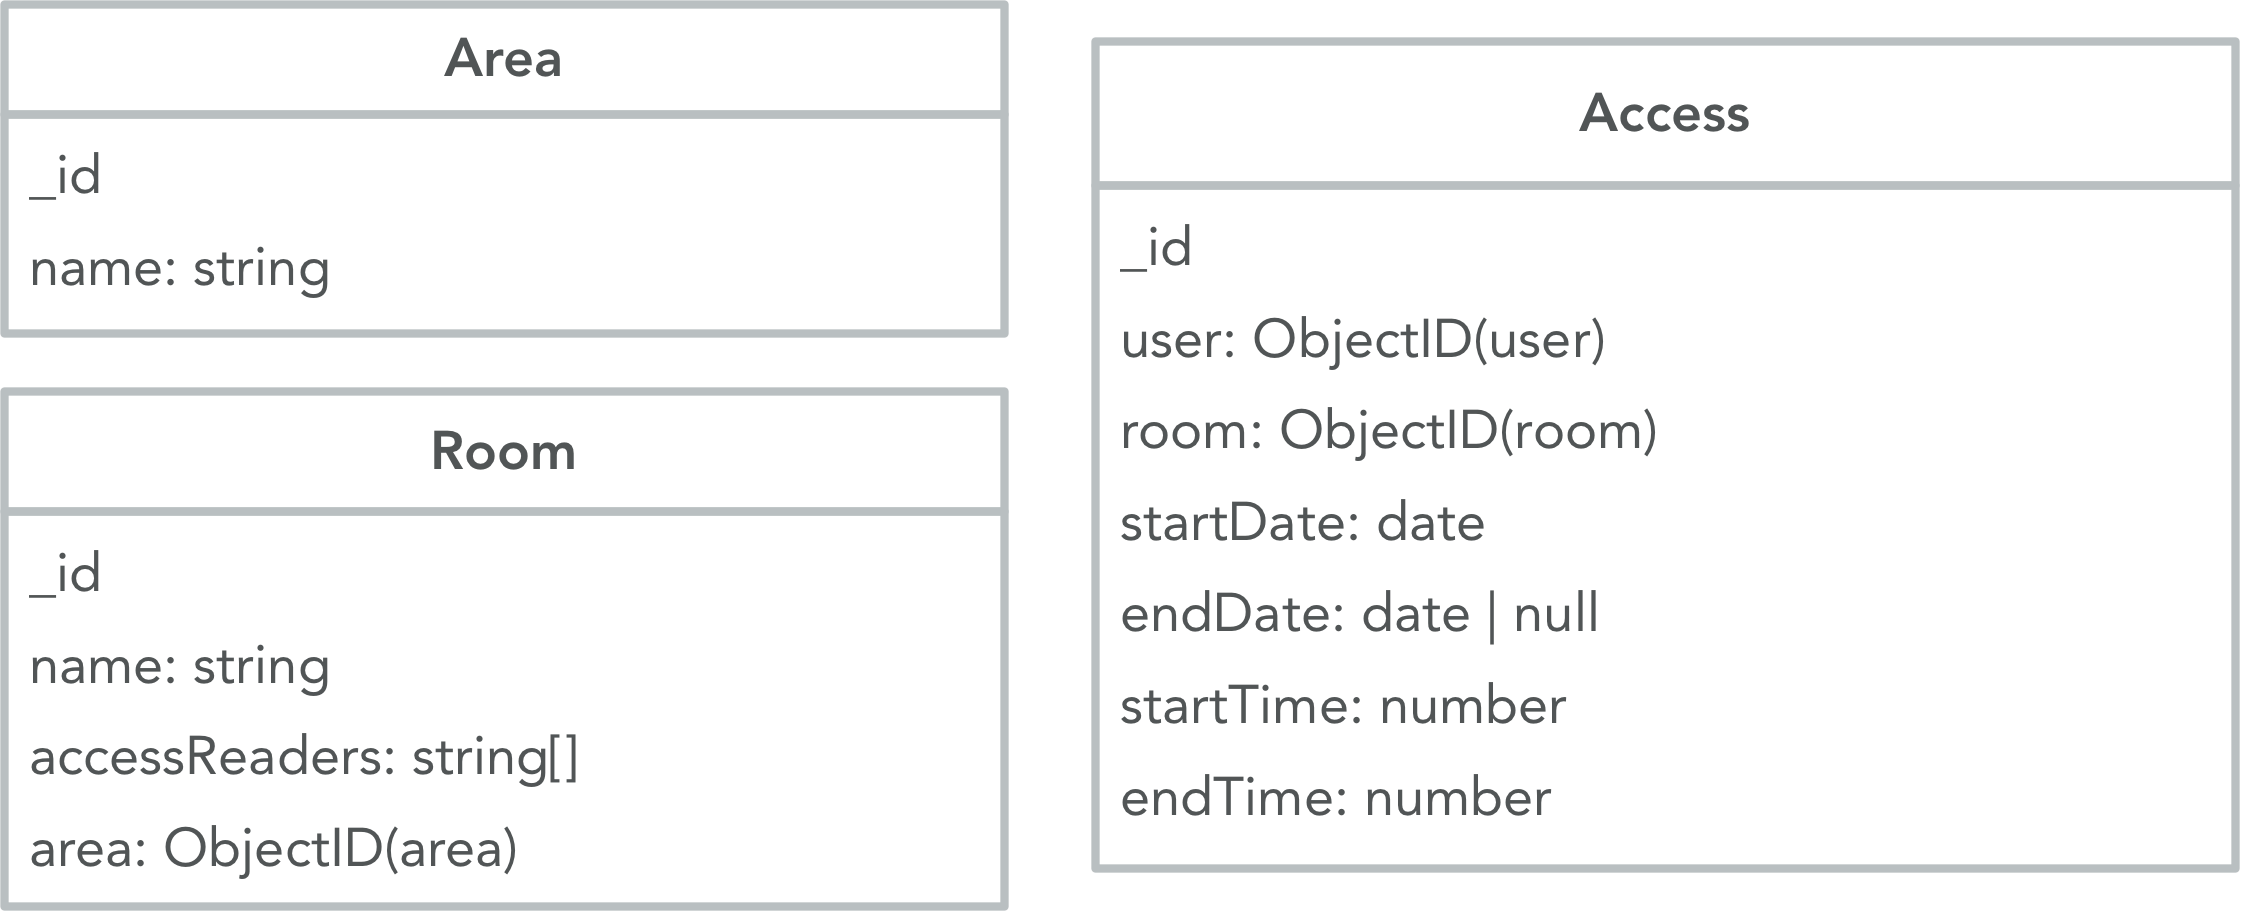
\includegraphics[width=.8\textwidth]{assets/access_model}
	\caption{The three models handling accesses}
\end{center}
\end{figure}

The access part of PocketHepia is composed of three models. We defined Areas, Rooms and Accesses. An area contains multiple rooms and each room has a specific set of accesses. Similarly to the payments model, we reference from the child to the parent with the ID of the parent. The room has the id of the area it is part of, and the access stores the id of the user and the room. \\

When deleting an area, we delete all rooms contained in that area. When deleting a room, we delete all accesses associated with the room. This is done using Mongoose hooks (see section \ref{mongoose_hooks}) to ensure that on every removal, we cascade it through the children.
%%\subsubsection{Access requests}
%%\subsubsection{Access logs}
\subsection{Logs}
\begin{figure}[H]
\begin{center}
	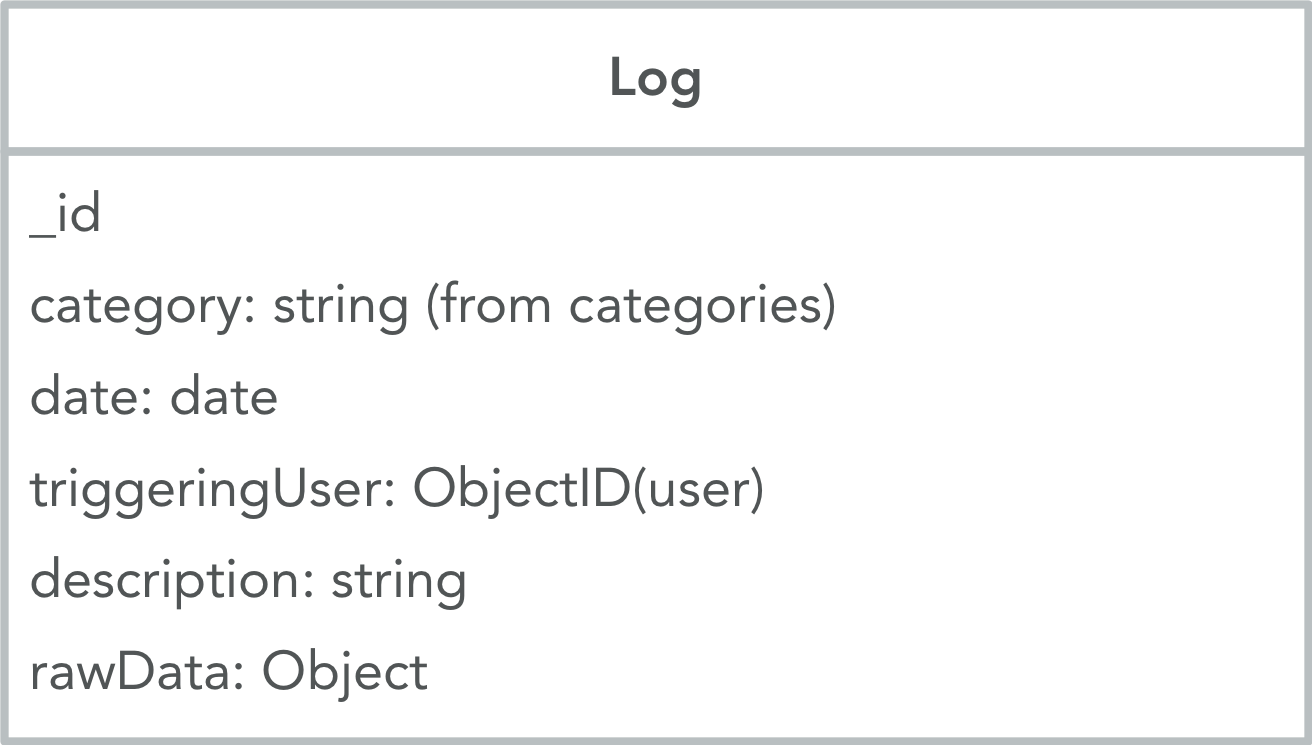
\includegraphics[width=.6\textwidth]{assets/log_model}
	\caption{Log Model}
\end{center}
\end{figure}
Finally, we decided to log all administrative actions and make the logs visible to all admins on the website. Giving access to a room or creating a new account can be sensitive, so we have to keep an historic of those actions.\\

We defined a Log model to store the logs in the DB and several log categories to distinguish the different logs and filter them.

The log categories are:
\begin{itemize}
\item User creation
\item User changes its password
\item User deleted
\item Admin imports users
\item Admin cancels an import
\item Admin assigns a \gls{nfc} Tag
\item Admin removes a \gls{nfc} Tag
\item Admin adds money to a user balance
\item Admin resets a user password
\item Admin changes a user permissions
\item Admin creates an area
\item Admin deletes an area
\item Admin creates a room
\item Admin deletes a room
\item Admin gives an access
\item Admin removes an access
\end{itemize}
As well as categories for features we will not implement yet:
\begin{itemize}
\item Admin delegates an area
\item Admin removes an area delegation
\item Admin completes an access request
\item Admin deletes an access request
\end{itemize}

The category for a log entry is stored as a \verb+string+ and we setup validation on the model to ensure the \verb+string+ used corresponds to a category.\\

We also store an embedded object we call \verb+rawData+, this allows us to store additional information specific to each category. For example for a permission change, we store the user before and after the changes. \\

Finally, the field \verb+triggeringUser+ stores the id of the user that did the action, we can then filter the logs to find out everything a specific person did.
\section{User stories}
From the beginning, we wrote simple user stories as a roadmap for the project features we wanted to implement. All of these features are not part of this academic project but are part of the broader student card project. 
%% TODO Continue text, references the table
%% TODO talk about features implemented during the summer, they will be explained in the report how to implement them and then implemented outside the project for the demo

\renewcommand*{\arraystretch}{1.5}
\begin{longtable}[c]{|p{0.33\linewidth}|l|p{0.33\linewidth}|}
\hline
\textbf{User story name}                                                                                                                       & \textbf{Priority} & \textbf{Status as of July 11th 2018}                \\ \hline
\endhead
%
User must be able to login using username and password (then using \gls{jwt} to communicate with backend)                                            & 1 - Essential     & Done                                             \\ \hline
Admin can create users from the website                                                                                                        & 1 - Essential     & Done                                             \\ \hline
User can view its total balance and a summary of its information on the homepage (web and application)                                         & 2 - Important     & Balance card done, other information in progress on web, Android done                                             \\ \hline
User can view all its transactions on the transactions page (web and application)                                                              & 2 - Important     & Done                                             \\ \hline
User can view its total balance on the transactions page (web and application)                                                                 & 2 - Important     & Done                                             \\ \hline
User can view all its accesses to rooms on the access page (web and application)                                                               & 2 - Important     & Done                                             \\ \hline
Admin can delete users from the website                                                                                                        & 2 - Important     & Done                                             \\ \hline
Admin can reset password for all users from the website                                                                                        & 2 - Important     & Done                                             \\ \hline
Admin can create users in batch by importing a CSV file                                                                                        & 2 - Important     & Done                                             \\ \hline
Admin can create areas from the website                                                                                                        & 2 - Important     & Done                                             \\ \hline
Admin can create rooms from the website                                                                                                        & 2 - Important     & Done                                             \\ \hline
Admin can give access to a room for a user from the website (start/end date and timerange)                                                     & 2 - Important     & Done                                             \\ \hline
Admin can remove an access from the website                                                                                                    & 2 - Important     & Done                                             \\ \hline
Admin can view all accesses for a user                                                                                                         & 2 - Important     & Done                                             \\ \hline
Admin can view all accesses for a room                                                                                                         & 2 - Important     & Done                                             \\ \hline
Admin can assign a physical card to a user from the Android app                                                                                & 2 - Important     & Done                                             \\ \hline
Admin can remove a physical card for a user from the Android app                                                                               & 2 - Important     & Done                                             \\ \hline
Admin can view all administrative logs from the website and filter them                                                                        & 2 - Important     & Done                                             \\ \hline
All administrative actions should be logged                                                                                                    & 2 - Important     & In progress (all implemented actions are logged) \\ \hline
User having the “Accept Payment” permission can create a payment from the Android app and scan a user card to validate the payment             & 2 - Important     & Done                                             \\ \hline
User can change its password                                                                                                                   & 3 - Normal        & Done                                             \\ \hline
User can send money to another user from the Android app                                                                                       & 3 - Normal        & Done                                             \\ \hline
Admin can undo a user batch import                                                                                                             & 3 - Normal        & Done                                             \\ \hline
Admin can delete areas from the website                                                                                                        & 3 - Normal        & Done                                             \\ \hline
Admin can delete rooms from the website                                                                                                        & 3 - Normal        & Done                                             \\ \hline
Admin can change permissions of users from the website                                                                                         & 3 - Normal        & Done                                             \\ \hline
Admin can add money to a user account                                                                                                          & 3 - Normal        & Done                                             \\ \hline
User can view all its borrowed books on the books page                                                                                         & 4- Nice to have   & Not started                                      \\ \hline
All accesses should be logged                                                                                                                  & 4- Nice to have   & Not started                                      \\ \hline
User can add money to its account using its credit card (using Stripe)                                                                         & 4- Nice to have   & Frontend in progress                             \\ \hline
User can create a virtual card from the application and use it                                                                                 & 4- Nice to have   & Placeholder and navigation on Android only       \\ \hline
User can request access to a room from the website                                                                                             & 4- Nice to have   & Not started                                      \\ \hline
Admin can delegate admin rights for an area to a user                                                                                          & 4- Nice to have   & Not started                                      \\ \hline
Admin can view and mark as done room access requests                                                                                           & 4- Nice to have   & Not started                                      \\ \hline
Auditor should be able to view access logs                                                                                                     & 4- Nice to have   & Not started                                      \\ \hline
Auditor should be able to view all payments logs                                                                                               & 4- Nice to have   & Not started                                      \\ \hline
User having the “can invite” permission can create a temporary user from the Android app and the website                                       & 4- Nice to have   & Not started                                      \\ \hline
User having admin rights for an area can give access to an user to a room in that area (start/end date and start/end hour)                     & 4- Nice to have   & Not started                                      \\ \hline
User having admin rights for an area can view and mark as done room access requests for that area                                              & 4- Nice to have   & Not started                                      \\ \hline
Onboarding setup process in web frontend to create first user when no users exists in the DB                                                   & 4- Nice to have   & Not started                                      \\ \hline
Ability to connect to LDAP (Active Directory for example) for users and authentication                                                         & 4- Nice to have   & Not started                                      \\ \hline
Librarian can create a loan for a book for a user from the Android app                                                                         & 5 - Not relevant  & Removed                                          \\ \hline
Librarian can view current bookings for all users from the website and Android app and mark the borrowing as Complete (all history on website) & 5 - Not relevant  & Removed                                          \\ \hline
\caption{User stories}
\label{user_stories_table}\\
\end{longtable}


\section{Technological choices}
\label{technological choices}
\subsection{The data and backend}
For the data and backend part of the project, we decided to build a unique backend for both the web and mobile clients. We would need a database to store the data of our models and a service to access to access that data. The easier solution would be to build a \gls{rest} \gls{api} in front of a database. To do this, we saw two main possibilities: a PHP \gls{rest} \gls{api} coupled with a \gls{sql} Database or a Node.JS Express \gls{rest} \gls{api} coupled with a Mongo DB. While we could mix these and use a \gls{sql} Database with Node.JS, we wanted to use the better affinity possible between the two. With the increase in popularity in Javascript based backends, we decided to rule out the PHP option and keep the Express/Mongo option. This is also due to the fact that PHP feels dated and does not provide a clear structure unless you use a PHP Framework to complement it. \\

The second solution that was suggested was to use an object syncing platform to directly synchronise data with all of our clients. One of these platforms is \emph{Realm Platform\footnote{\url{https://realm.io/products/realm-platform}}} and we decided to study the advantages of it for our project and decide if we should use it over the Express/Mongo option.
\subsubsection{Realm vs. Express-MongoDB}
\begin{figure}[H]
\begin{center}
	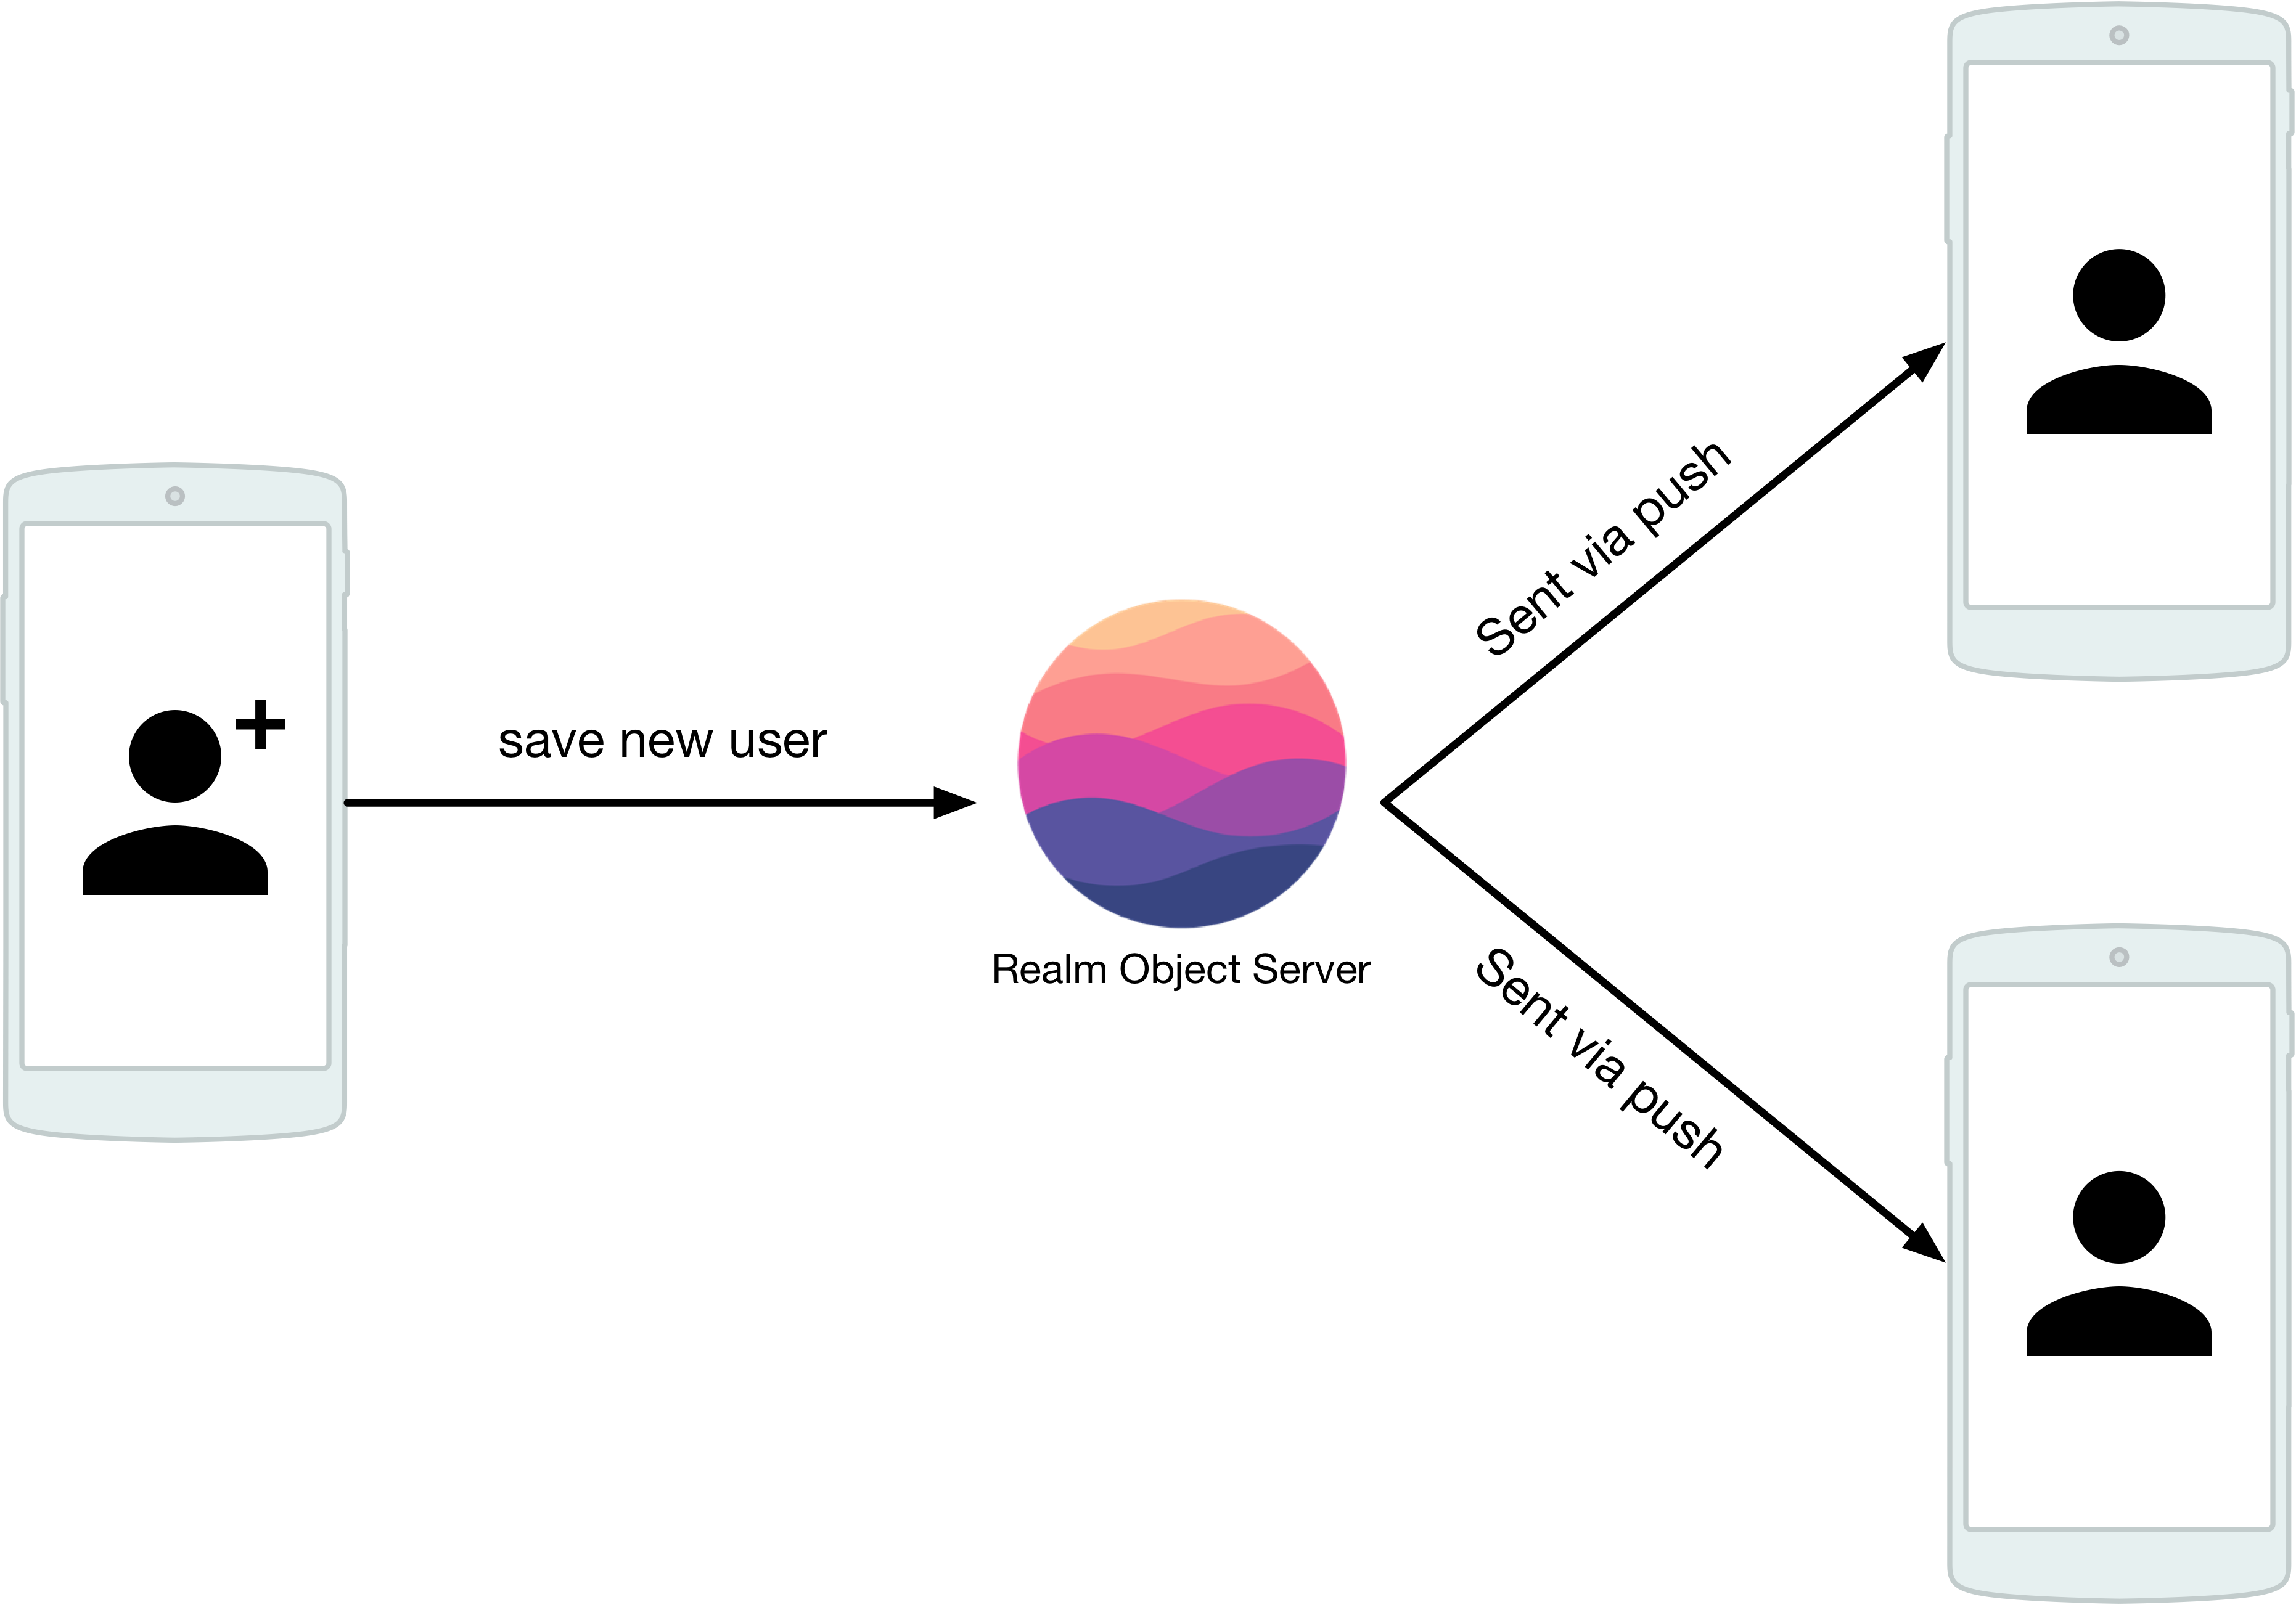
\includegraphics[width=.8\textwidth]{assets/realm_architecture}
	\caption{Saving an object in Realm}
	\label{realm_object_saving_figure}
\end{center}
\end{figure}

\begin{figure}[H]
\begin{center}
	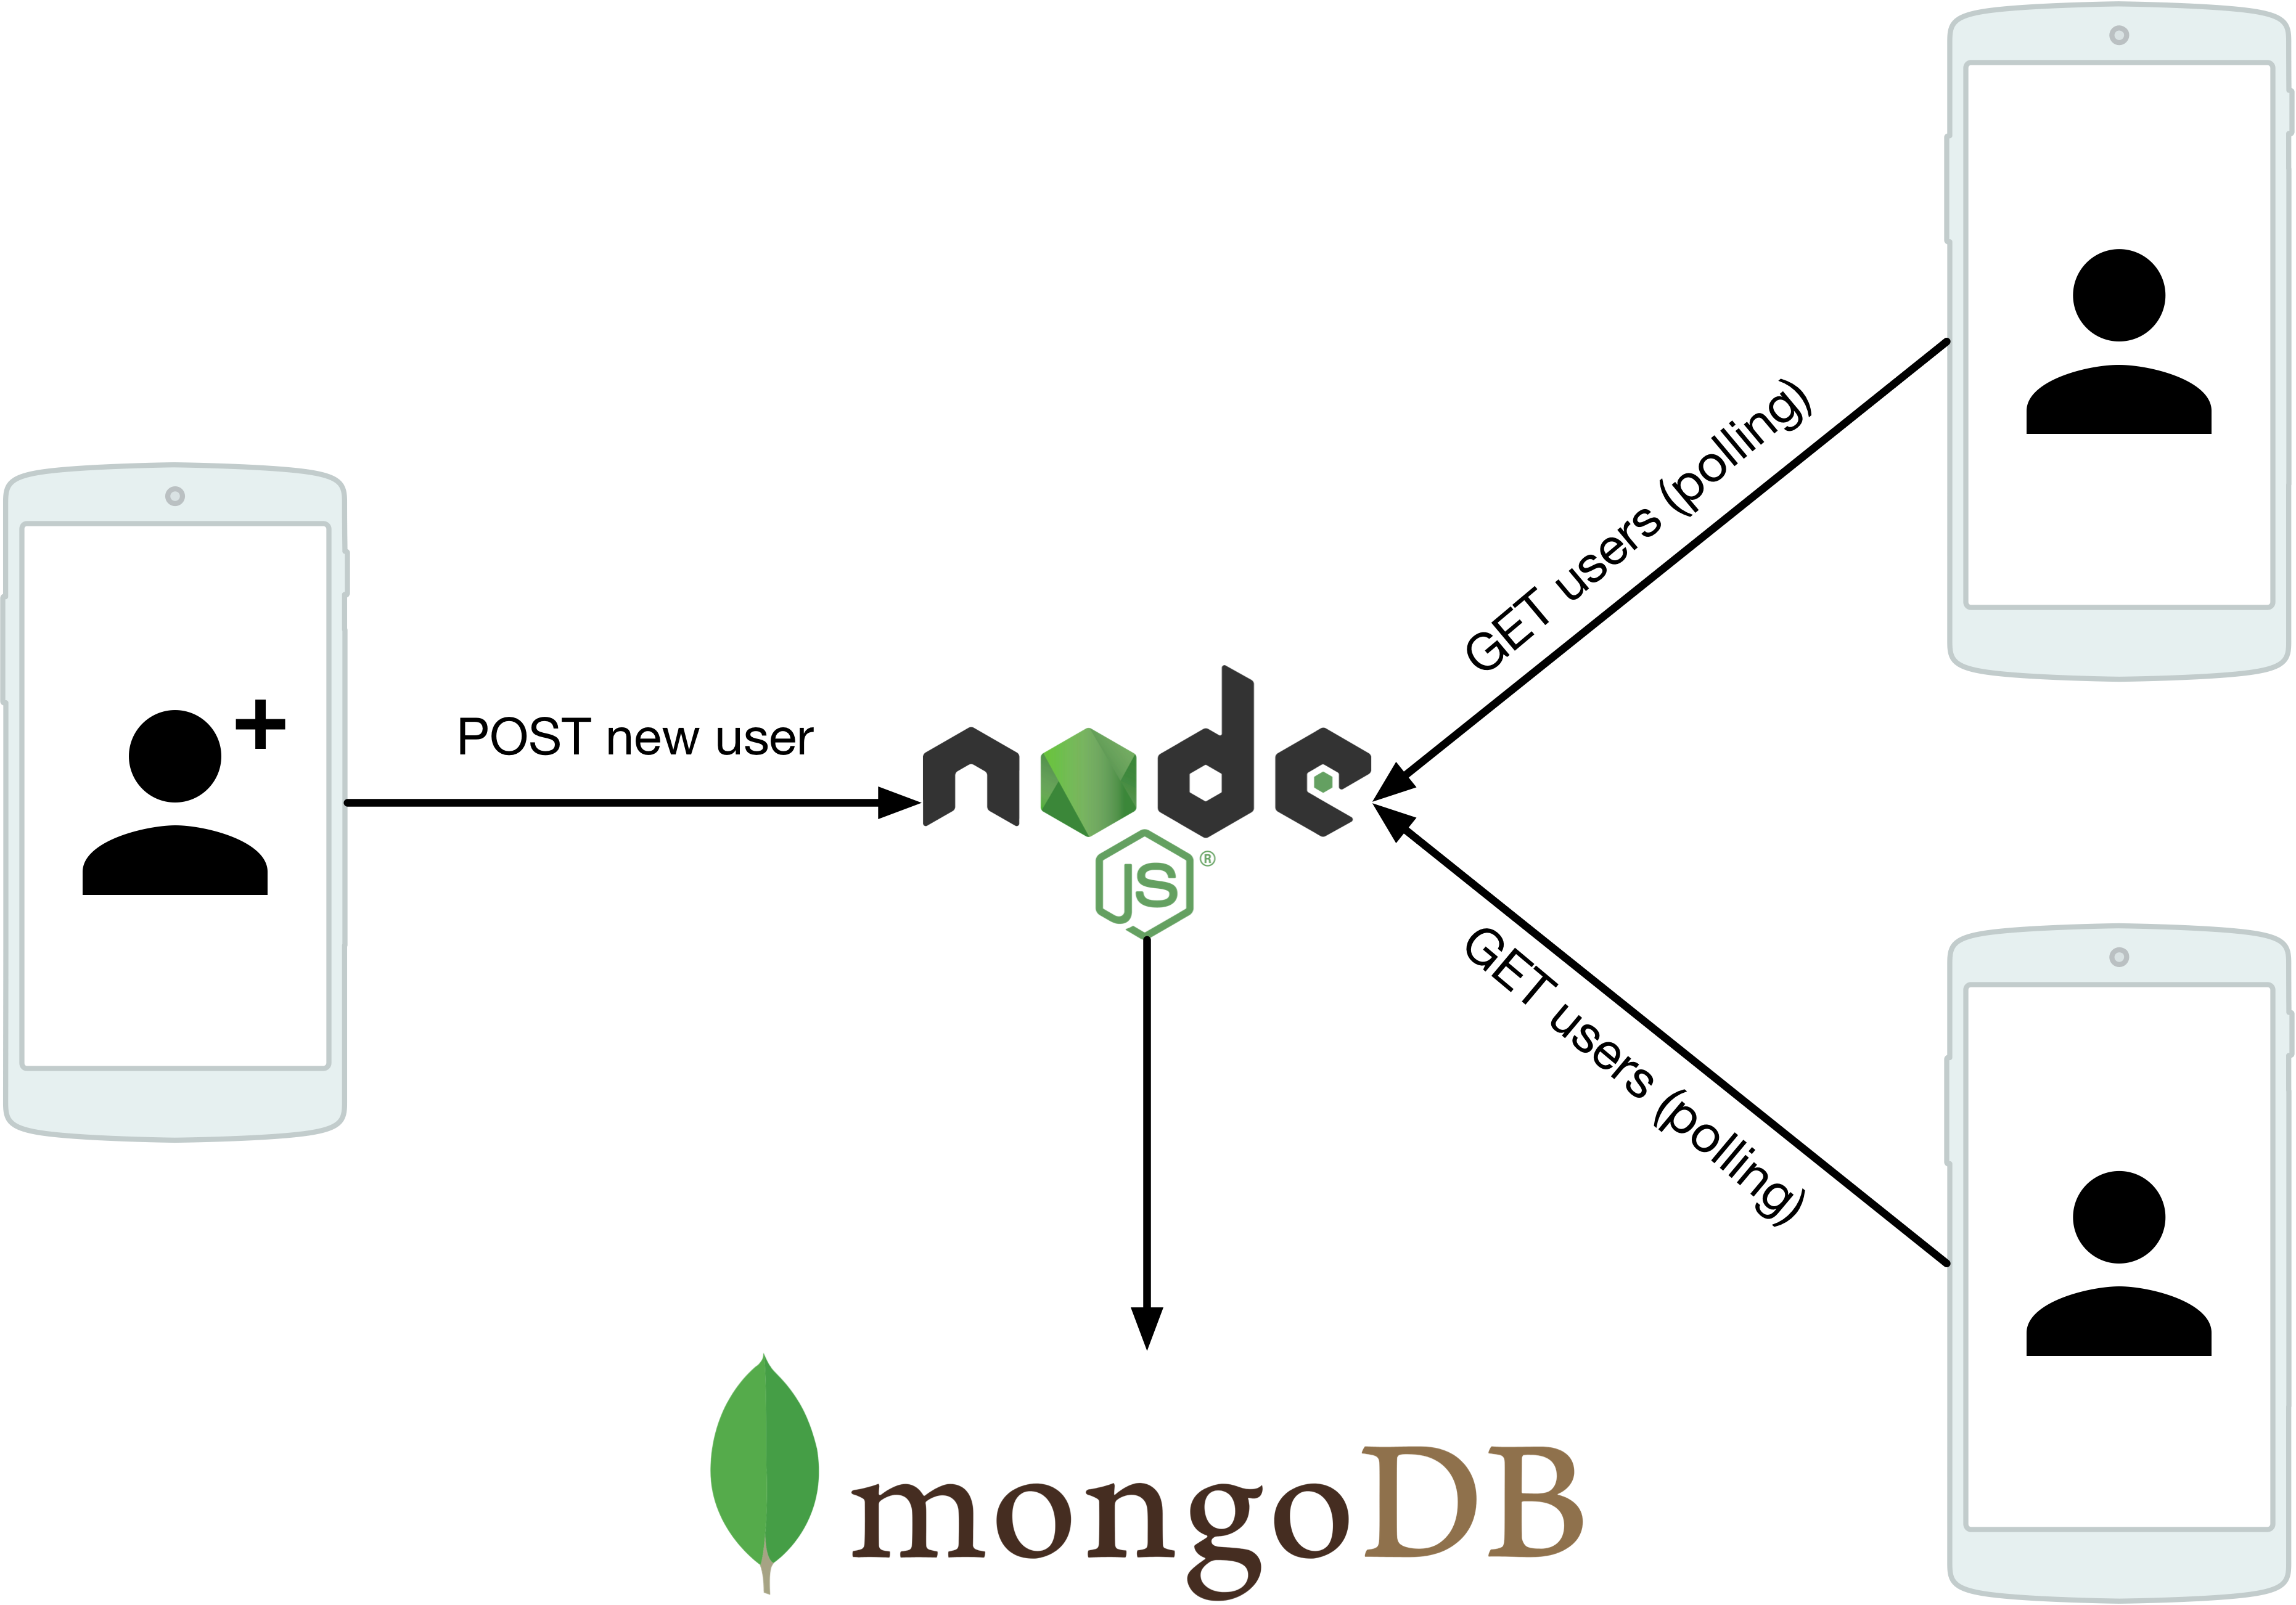
\includegraphics[width=.8\textwidth]{assets/expressmongo_architecture.png}
	\caption{Saving an object in Express/Mongo}
		\label{mongo_object_saving_figure}
\end{center}
\end{figure}
The Realm platform integrates the database directly within an object server that takes care of providing access and sending data to all the clients connected to it. This is possible thanks to the Realm runtime that you need to integrate in your client-side application and will replicate the database server on your local client.\\

On the contrary, using the Express/Mongo approach, we have the Mongo database and we built a \gls{rest} \gls{api} in front of it to provide access to the data. We do not need any particular runtime on the client-side and we can just handle data how we want. \\

As we can see in figures \ref{realm_object_saving_figure} and \ref{mongo_object_saving_figure}, when we create a new object on a client in Realm and save it locally, it is directly sent to the server and then pushed to other devices without needing any action. On the Express/Mongo side, you save the new object to the server and then other clients can retrieve it. \\
\paragraph{Advantages of Realm}
The advantages of Realm apply mainly on the mobile front. Realm is built to the ground up for the constrained resources and connectivity of mobile devices. It is offline first and will cache changes to be sent to the Realm server when the connection is back. Moreover, the push synchronisation of data back to the clients is the most efficient way to retrieve new data as opposed to polling data from a server at a regular interval.
\paragraph{Only for specific use cases}
The problem with Realm is that, beyond mobile, it is not very appropriate for our project. There are many pain points and small decisions that were taken by the Realm team that impose a way of doing things that may not be compatible with every project.\\

For example, one of these problems is the user authentication part and the user collection. In Realm, a user is not an object like others. It is a special object that is also used to connect to the Realm engine to handle sync. So you are limited to using Realm authentication to use the platform. Moreover, there is no way for a user with admin rights to retrieve a list of users on the client-side. This data is not accessible, unless you use the Realm Studio \gls{gui} client.\\

Another point is that, since you directly interact with the database/object server on the client-side, the code can easily be changed to access other people's information unlike a \gls{rest} \gls{api} where access to the database is regulated by the \gls{api}. To avoid this, Realm has a system of permissions that are assigned to saved objects, but you need to assign the permissions every time you create a new object. Admins do not have direct access to everything, so you also have to add a permission for every admin every time. We wouldn't even imagine trying to add multiple set of roles here, it would be too cumbersome to handle.\\

Finally, the final point that made us abandon Realm for this project is the lack of clear solution to use it on the web. You have two ways to access the data from a web client. Either activate the GraphQL integration and write GraphQL queries to interact with the data from the web frontend. Or use the Node.JS Realm runtime to connect to the object server and serve as an \gls{api} to access the data. So, even if we used Realm, we would still need to write an \gls{api}. We're better off just going with the Express/Mongo option in that case. \\

It is a shame because the product provide real advantages on mobile that would take time to implement with a custom data solution, but it just isn't flexible enough and is really mobile-first while the web seems a bit like an after-thought for them. Even in their marketing material, they only present mobile-only applications such as chat or photo-sharing applications.

%%TODO add ref for Realm Studio and GraphQL explanation with footnote and ref
\subsection{Mobile application}
We needed to create a mobile client to access the information and status of a users' data from a smartphone as well as complete some administrative tasks. \\

We decided to build an Android application as well as coding the website to be responsive so it can be used on any smartphone. For the standard user, the mobile application is the one to use as it will provide access to all information, sync data offline and enable payments to other users. For the administrators, the mobile application will allow them to manage physical cards for users and for the rest of the administration, they can use the website on their smartphone.
\subsubsection{Why the need for an application?}
While we could have achieved most of the functionality with a web application, there are still some elements that require building a full mobile application. Mainly, access to device features such as \gls{nfc}. With a mobile web app, we cannot have access to the \gls{nfc} chip on the smartphone and thus we cannot manage physical cards or make payments through the app. This is also the reason why we only built an Android app and not an iOS one. The \gls{api} for \gls{nfc} on iOS\cite{apple:ios:nfc} is basic and was released in 2017, it does not allow writing on \gls{nfc} tags\footnote{Unless you are a big company partnering directly with Apple} and only supported a subset of the formats of the Android \gls{api}.\\

Apart from this limitation, all the other functionality could have been incorporated in a web application, for example by making a Progressive Web App (PWA)\cite{google:pwa:website}. PWA are an hybrid between a mobile application and a web application and they run on desktop and mobile operating systems. Their main advantages compared to traditional web app is that they can be "installed" on the device and act like a normal application and that they generally store data offline and can sync data in the background through the user of Service Workers.
\subsubsection{Why go native?}
We could have also found a middle ground between the mobile web application and the native web application by using a mobile application framework such as Ionic or React Native to build our mobile application using web technologies. This would have allowed us to reuse some components built for the web in our mobile application.\\

We decided to opt out of that route and build our application using native Android technologies to better take advantages of the cutting-edge features announced during Google I/O 2018 \footnote{Google I/O is the annual Google developer conference held in June for developers using Google technologies (Chrome, web, Android, iOS,...), \url{https://events.google.com/io/}} aiming to modernise and improve the Android development workflow (see section \ref{android_chapter}).
\subsection{Web Frontend}
Finally, we opted to use a frontend framework to provide a good structure to our client-side web application instead of relying on static custom HTML/CSS/JS.\\

The three main frameworks available at the moment are Angular\footnote{There is a distinction to be made between AngularJS (Javascript) and Angular.io (Typescript). While both coexist, you should use Angular.io as it is the version that is developed going forward. In this document, we will be talking about Angular.io when mentioning Angular}, React and Vue. \\

Vue is the youngest of the three and, while it is already growing a big community, its documentation is not as complete as the two others and its also growing rapidly which means that some of our code might become obsolete rapidly. \\

React and Angular are more mature, with Angular being the oldest of the three and are both baked by big companies: Facebook for React and Google for Angular. The biggest difference between the two is that React is Javascript-based and Angular is Typescript-based. We decided then to use Angular to take advantage of the typed nature of Typescript as well as to use Typescript for the first time in a project. \\

\subsection{MEAN Stack}
By using MongoDB with Express/Node.js and Angular, we are effectively using the \emph{MEAN}\footnote{Stands for Mongo-Express-Angular-Node}\cite{mean:website} development stack which is regarded as the more modern equivalent to the \emph{LAMP}\footnote{Stands for Linux-Apache-MySQL-PHP}\cite{wiki:lamp} stack. The \emph{MEAN} stack also has several variants where Angular is replaced by another frontend framework like React or Vue.

\chapter{Technologies}
In this chapter, we are going to present in more details the technologies that we used during this project. We will write more detailed sections about Android (see \ref{android_chapter}) because of all the new improvements that we decided to use and we studied for this project as well as Angular (see \ref{angular_chapter}) since we learned how to use it as part of this project. Those two technologies represented the most amount of work for this project. The other technologies used, NoSQL Databases and Node.JS will be described more briefly.
\section{Developing for Android}
\label{android_chapter}
Android is a mobile operating system developed by Google and launched in September 2008. The core of Android is open source and is known as the \emph{Android Open Source Program (AOSP)}. But nobody really knows or uses the AOSP version of Android, every phone manufacturer, even Google, forks the AOSP version to build its own for their devices. What is often referred as "pure Android" is the Google implementation of Android on their Nexus and Pixel lines of smartphones. Android runs on all kinds of platforms, from mobile phone to watches, as well as tablets and laptops. \\

A \gls{sdk} and an \gls{ide} are provided for developing Android applications. Those applications are written mainly in Java, with the ability to write native code in C++ using the Android NDK\footnote{This is used for example to use some C++ libraries, like OpenCV.} and interact with the Java code using JNI. The support for a second language named Kotlin was announced at Google I/O 2017 (see section \ref{kotlin}). Applications run in a virtual environment on Android called ART. You can think of ART as the equivalent of the \gls{jvm} for desktop Java development.
\subsection{Android Fragmentation}
One of the biggest problems for developers is the fragmentation of \gls{os} versions running on Android devices. As of May 2018, only 62.3\% of devices were running Android Marshmallow (version 6) or later. Android Marshmallow was released in 2015, meaning that 37.7\% of devices were running software that was more than 3 years old without security updates or new features (see table \ref{android_os_table}).

\begin{table}[H]
\centering
\bgroup
\def\arraystretch{1.5}%  1 is the default, change whatever you need
\begin{tabularx}{\textwidth}{|c|l|X|X|}
\hline
  \textbf{Year} & \textbf{Version Name} & \textbf{Usage of this version} & \textbf{Usage of this version or later}\\
  \hline
2010 & Gingerbread & 0.3\% & 100.0\% \\
\hline
2011 & Ice Cream Sandwich & 0.4\% & 99.7\% \\
\hline
2012 & Jelly Bean & 4.3\% & 99.3\% \\
\hline
2013 & Kit Kat & 10.3\% & 95.0\% \\
\hline
2014 & Lollipop & 22.4\% & 84.7\% \\
\hline
2015 & Marshmallow & 25.5\% & 62.3\% \\
\hline
2016 & Nougat & 31.1\% & 36.8\% \\
\hline
2017 & Oreo & 5.7\% & 5.7\% \\
\hline
\end{tabularx}
\egroup
\caption[Android OS Fragmentation]{Android \gls{os} Fragmentation (May 2018)\cite{android:dev:osfragmentation}}
\label{android_os_table}
\end{table}

\subsubsection{The problem with updates}
This problem is inherent to the very nature of the Android operating system. Each phone manufacturer, or OEM, can fork its own version of Android and integrate its own skin and set of apps on top of it. When a new version of the operating system is released by Google, they can't just start using it. They have to first adapt and test all their apps and customisation with the new version before it can ship to the devices. This is a time (and by extension money) consuming process and many OEMs just don't care about maintaining their devices for more than one or two years. To make matters worse, in certain countries, such as the United States, mobile carriers have to validate and apply their own custom apps and settings on top of the \gls{os}, adding to the time needed to validate an update and causing a supplementary potential roadblock to the release of an update.

\subsubsection{What Google is doing about this?}
Google has in the recent years taken different actions to ensure that most of the devices run safe and up-to-date software on them without depending on the OEMs willingness to maintain their products.
\paragraph{Updating core apps through the Play Store}
One of the most successful changes to Android in recent years has been to slowly move all Android core applications that are present on every Android device\footnote{Actually, not every Android device. Some Asian markets, mainly China don't have access to these apps because they don't have access to any Google services. This is an edge case that won't be discussed in this document. } to the Google Play Store. These apps include for example Gmail, Google Calendar, the browser (AOSP browser and Google Chrome) and even apps like the Phone Dialer and Contacts apps. This move to the Play Store allows Google to update these applications more frequently without needing a full operating system update. While it may be seen as a necessary evil at first, because it is the only way for them to update these apps if the OEM don't apply operating system updates, it is actually a very useful move because it allows for faster iteration on these applications and quicker response for bug fixes.\\

If we compare this to the other major mobile operating system, iOS, all main applications on the platform are bundled with the \gls{os}. So, if Apple needs to update the Safari browser to support a new web \gls{api} they have to release a full \gls{os} version and push it to all their devices instead of just updating the application that needs an update as Google would do on Android.
\paragraph{Android Support Library}
The Android Support Library is a set of libraries used to build applications on Android. Due to the \gls{os} fragmentation problem, the Support Libraries have been created to built features and add support for older versions of the \gls{os}. For example, you should prefer using \verb+AppCompatActivity+ instead of \verb+Activity+ when defining new Activities as the compatibility version, as its name suggests, will support a wider range of devices.\\

The Support Libraries packages were originally named using the earliest \gls{sdk} level supported by the library, such as \verb+android.support.v7.app+, but they never got updated to new names even after compatibility was dropped in order not to break imports in existing apps. This creates a confusion, because \verb+v7+ does not actually support API 7 minimum, but API 14. Starting in 2018, the Android team has decided to rename the packages from these libraries to remove a version support number using the \verb+AndroidX+\cite{android:doc:androidx} naming scheme. A refactoring tool will be integrate in Android Studio to convert a project to the new naming scheme.
\paragraph{Project Treble}
Another project designed to improve the adoption of new updates is \emph{Project Treble}. The idea behind the project was to split the \gls{os} from the manufacturer customisations so that the \gls{os} could be updated without needing to upgrade the customisations and they would run automatically on the new \gls{os}. While some small OEMs started integrating \emph{Project Treble}, most big manufacturers, including Samsung, simply do not care about its benefits.
\subsection{Kotlin}
\label{kotlin}
As discussed in section \ref{android_chapter}, Kotlin has become a primary Android language in 2017. After having used this language for a first Android project last year, I decided to build all my subsequent Android application in Kotlin. The simplifications and reductions in code length provided by this language compared to Java make developing Android applications more enjoyable. It also helps avoid many runtime errors by catching many error-prone scenarios at compile time. In this section, we will go in further details in some of the advantages provided by Kotlin and how Google is encouraging developers to use Kotlin by introducing new Kotlin-specific features in the Android \gls{sdk}.
\subsubsection{Full interoperability with Java}
First of all, the fact that Kotlin is fully compatible with Java and runs on the \gls{jvm} allows it to be easily integrated in an existing project or interact with existing Java libraries. You can just start writing classes in Kotlin and call existing Java classes from it and vice-versa. Then, when you want to convert Java code to Kotlin, Android Studio integrates a tool to convert a file to Kotlin almost perfectly. There are just some small changes to write afterwards, for example concerning the conversions of variables to constants. The \gls{ide} will even suggest converting Java code pasted inside a Kotlin file to the Kotlin version of the code.
\subsubsection{Data classes}
Java is often defined by its detractors as a very verbose language, requiring to write a lot of repetitive boilerplate code\footnote{Boilerplate code or boilerplate refers to sections of code that have to be included in many places with little or no alteration\cite{wiki:define:boilerplate}} for simple tasks. One of these tasks is the creation of classes with accessors and mutators for some of the class fields and overriding \verb+equals+ and \verb+toString+ methods. In Object Oriented Programming, we often have to write a lot of small classes just to match the Models in our applications. These are often referred as Beans or POJOs\footnote{Plain Old Java Object}. Kotlin introduces the concept of data classes\cite{kotlin:doc:data_classes} to simplify the implementation of these type of classes. By using a data class, you get "for free" an accessor (and mutator) for each field of the class, a correct overriding of the \verb+equals+ method, an overriding of the \verb+toString+ method listing the values of all fields in the instance and a \verb+copy+ method corresponding to a copy constructor in Java. For example, if we take a simple person class in Java:
\begin{code}
\javacode{assets/code/java/Person.java}
\caption{Person class implementation in Java}	
\end{code}

And then the same class written using data classes in Kotlin:
\begin{code}
\kotlincode{assets/code/kotlin/Person.kt}
\caption{Person class implementation in Kotlin using Data Classes}	
\end{code}
\subsubsection{Constants first}
As in Java, you can define variables and constants in Kotlin but, in the later you will be more inclined to use constants because you can use them in more cases and the compiler suggests using constants when it detects that a variable is never assigned a new value. To use a constant, you use the keyword \verb+val+ instead of \verb+var+. \\

One example of a case where you can use a constant in Kotlin but not in Java is when using blocks such as try/catch or control flow blocks. In Kotlin, these blocks return a value so you can assign the value returned by the block to a constant. The value returned by a block is the last line of the block or the last line of the taken branch of a control flow block\cite{kotlin:doc:controlflow}. \\

For example, let's say that we are parsing a \verb+String+ as an \verb+Integer+ and we want to check if the value is between a given range. When parsing, an Exception can be returned if the value is not a number, so we have to be aware of that.\\

In Kotlin, we can directly assign the value of the whole try/catch block to the constant:
\begin{code}
\kotlincode{assets/code/kotlin/ConstantsFirsts.kt}
\caption{Assigning values returned by control blocks in Kotlin}	
\end{code}

However, in Java, we have to define a variable first and then we have to reassign it according to the branch we are in:
\begin{code}
\javacode{assets/code/java/ConstantsDemo.java}
\caption{Assigning values with control blocks in Java}	
\end{code}
\subsubsection{Class extensions}
Another advantage of Kotlin is the ability to write class extensions\cite{kotlin:doc:extensions}. This is useful to add methods to classes present in libraries for example and is used extensively as part of the Android KTX project (see section \ref{ktx_section}).\\

For example, if we are using the \verb+ByteArray+ class and we want to convert the value to a hexadecimal \verb+String+, we can write a class extension method or property for the \verb+ByteArray+ class that we can then call on any instance of the class.

This is done in this way:
\begin{code}
\kotlincode{assets/code/kotlin/Extensions.kt}
\caption{Defining method and properties extensions in Kotlin}	
\end{code}


And can then be called like any methods or properties:
\begin{code}
\kotlincode{assets/code/kotlin/ExtensionsUsage.kt}
\caption{Using method and properties extensions in Kotlin}	
\end{code}

\subsubsection{Null safety}
In terms of safety, Kotlin introduces concepts already seen in other languages such as Scala or Swift but not present in Java, mainly around the handling of \mintinline{java}{null} values\cite{kotlin:doc:null}.\\

In Java, if a function returns a \mintinline{java}{String} or another \mintinline{java}{Object}, it can also return a \mintinline{java}{null} value and if we forget to check if the value is not \mintinline{java}{null} and try to access it, the program will throw a \mintinline{java}{NullPointerException} at runtime and it will certainly crash. Runtime errors are unexpected and can happen at anytime so they should be avoided at any cost. \\

In Kotlin, they introduce the concept of optional types, denoted by a \verb+?+. This allows for compile time check of \mintinline{java}{null} values risks. First of all, a function that returns a \mintinline{java}{String} can't return a \mintinline{java}{null} value. To return a \mintinline{java}{null} value you specifically have to return an optional type, in this case a \mintinline{kotlin}{String?}. This optional type can only be accessed after checking if it contains a non \mintinline{java}{null} value. After the check, it will be \emph{smart-casted} as \mintinline{kotlin}{String} in the corresponding code block. The program will not compile if an optional type is used without checking if it contains a value first which avoids the possibility of having \mintinline{java}{NullPointerException} at runtime\footnote{This is valid for Kotlin code. When interacting with existing Java code, the Java code can use annotations \mintinline{java}{@Nullable} and \mintinline{java}{@NotNull} to mimic optional types but they are not required annotations so you can still run into problems depending on the Java library. An error could also happen if we bypass the \mintinline{java}{null} safety check by using the \emph{not-null assertion operator}, see paragraph \ref{optional_operators_kt}} \\

For example, an usage of the optional types is a function that finds an element in a list and returns the index of the element in the list. If the element is not contained in the list, it will return a \mintinline{java}{null} value. The function should then return a \mintinline{kotlin}{Int?} and this value can only be used after specifically checking that the value is not \mintinline{java}{null}:
\begin{code}
\kotlincode{assets/code/kotlin/optional.kt}
\caption{Using optionals in Kotlin}	
\end{code}


\paragraph{Optionals-related operators}
\label{optional_operators_kt}
Kotlin also introduces a number of specific operators to handle optional types:
\begin{itemize}
	\item The \emph{not-null assertion operator}: This operator is \verb+!!+ and is used to tell the compiler that we unwrap the value from an optional without checking if it contains a value first. This is the \emph{living dangerously} operator.
	\item The \emph{safe call operator}: This operator is \verb+?+ and can be used when trying to access members and methods for optional types instances. It will return an optional type as well, for example if we have a \mintinline{kotlin}{user: User?} and we want to get its name, we can use \mintinline[breaklines]{kotlin}{val name = user?.name} and this will return the name of the user if the user is not \mintinline{java}{null} and otherwise will return \mintinline{java}{null}.
	\item The \emph{Elvis operator}: This operator is \verb+?:+ and is used to indicate a value to use if the value is \mintinline{java}{null}. For example, with the user's name before, \mintinline[breaklines]{kotlin}{val name = user?.name ?: "Paul"}. The "Paul" name will be used if the expression returns a \mintinline{java}{null} value
\end{itemize}

\subsection{NFC on Android}
If an Android device contains a \gls{nfc} chip, you can use the chip capabilities in an application. To do so, first of all, you have to add the request for permission to access it in the Android Manifest. The Manifest is the configuration file for the application from the \gls{os} point of view. It contains the listing of permissions, activities and other configuration. To use \gls{nfc}, you have to add the line \mintinline[breaklines]{xml}{<uses-permission android:name="android.permission.NFC" />}. \\

From there, you have two different possibilities that can also be combined. You can either register yourself to the \gls{os} to listen for any incoming \gls{nfc} actions (touching a tag for example) no matter if your app is running or not. You can also intercept \gls{nfc} actions when your app is in the foreground. In most cases, the latter solution is the one needed, unless you want your app to be launched when a specific \gls{nfc} accessory is detected. The foreground method is called \emph{Foreground dispatch}, it means we are filtering the intent that are received by our foreground Activity to include \gls{nfc} related intents and passing them to the Activity.

\subsubsection{Setting up \emph{Foreground Dispatch}}
You have to setup \emph{Foreground Dispatch}\cite{android:doc:nfc_foregroundDispatch} at the Activity level, preferably in the \mintinline[breaklines]{kotlin}{fun onCreate(savedState: Bundle?)} method and then enable it and disable on resume and pause of the Activity respectively. If you need to use it in multiple activities, it is easier to setup a superclass Activity and extends all other Activities from it. We can then just override the \mintinline[breaklines]{kotlin}{fun onNewIntent(intent: Intent)} in the specific Activity for which we need to handle \gls{nfc} specifically. In the superclass Activity, we can just discard the received \gls{nfc} intent.\\

As we can see in source code \ref{foreground_dispatch_code}, we have to register all technologies and intent types that we need to filter and create a pendingIntent to be sent by it. We activate the filter when the Activity is resumed and disable it when it is destroyed. This is to avoid blocking all other apps after our application quits and avoid crashes as well because if a \gls{nfc} action happens and our app gets it in the background, it will crash. When we get the \gls{nfc} intent, we just log a message by default and discard the intent.

\begin{code}
	\kotlincode{assets/code/kotlin/ForegroundDispatchActivity.kt}
	\caption{Foreground Dispatched superclass Activity}
	\label{foreground_dispatch_code}
\end{code}
\subsubsection{Getting a Tag ID}
Now, if we want to read a \gls{nfc} Tag inside an Activity, we just need to override the \mintinline[breaklines]{kotlin}{fun onNewIntent(intent: Intent)} method. For example, when assigning a Tag to a new \verb+User+, we have to get the \gls{nfc} Tag unique identifier and send it to our backend. To do that, we can use the following code:
\begin{code}
	\kotlincode{assets/code/kotlin/ReadNFCid.kt}
	\caption{Reading ID from NFC Tag}
\end{code}
\subsection{Android Jetpack}
Android Jetpack is a set of tools and libraries designed to improve the quality of Android applications by providing guidelines and code to implement common behaviours. Initially launched as \emph{Android Architecture Components} at Google I/O 2017, it has been renamed in 2018 and gained new features. The main goals of Android Jetpack are to accelerate development by providing adaptable common features, to help with tedious activities such as background work and lifecycle management that require a lot of boilerplate code\cite{wiki:define:boilerplate} and to improve the quality of applications by providing modern and robust core libraries.\cite{android:doc:jetpack}. You do not have to use Android Jetpack libraries but they can be seen as a set of good practices and tools to help development.
\subsubsection{Android KTX}
\label{ktx_section}
Android KTX is a Kotlin-specific part of Android Jetpack. It provides Kotlin extensions for Android and Jetpack libraries to take advantage of Kotlin features and make code more concise\cite{android:doc:ktx}. It is composed of different modules, each related to a library or use case on Android. KTX is also open source and actively developed on GitHub\cite{github:android:ktx}. You can contribute to it by creating new extensions or just suggesting them to the development team.\\

An example of Kotlin features used in KTX is the improvement to the usage of Lambdas and anonymous functions as well as the usage of these functions to avoid chaining calls.\\

For example, when replacing a fragment in a view, you can use a block with KTX in which you write the replacement operation and the block will begin and commit the transaction automatically:
\begin{code}
\kotlincode{assets/code/kotlin/fragmentsKTX.kt}
\caption{Handling Fragment transactions with Android KTX}	
\end{code}


Similarly when working with a SQLite Database and writing a transaction, the KTX version will take care of catching the exception and cancelling the commit if an exception is raised:
\begin{code}
\kotlincode{assets/code/kotlin/dbKTX.kt}
\caption{SQLite transactions with Android KTX}	
\end{code}

\subsubsection{Room - Data persistence}
There are three main ways to store persistent data in an Android application. First, you can use files, either user accessible files or files only available from the app code. Secondly, you can use \verb+SharedPreferences+ to store key/value pairs. And finally, you can use a database. Databases on Android are built on SQLite and have always been the best way to store data on Android. The problem though was that the code to write to use databases was too long and complex and you could easily run into errors due to the usage of bad practices or wrong \gls{sql} syntax for example. Moreover, you always had to parse the data returned from the database into models and vice-versa so it always felt like you had to do the work twice.\\

With Room\cite{android:doc:jetpack:room}, part of the Architecture section of Android Jetpack, the goal is to simplify the usage of SQLite databases by providing an abstraction layer on top of it. Used in conjunction with ViewModel and LiveData, it simplifies the handling and presentation of data on Android.\\

As seen in figure \ref{room_architecture_img}, the application interacts with the Room Database to get an instance of \gls{dao} and retrieve Entities. All of these are generated by the library, we just have to provide simple "configuration" classes and interfaces.\\
\begin{figure}[H]
\begin{center}
	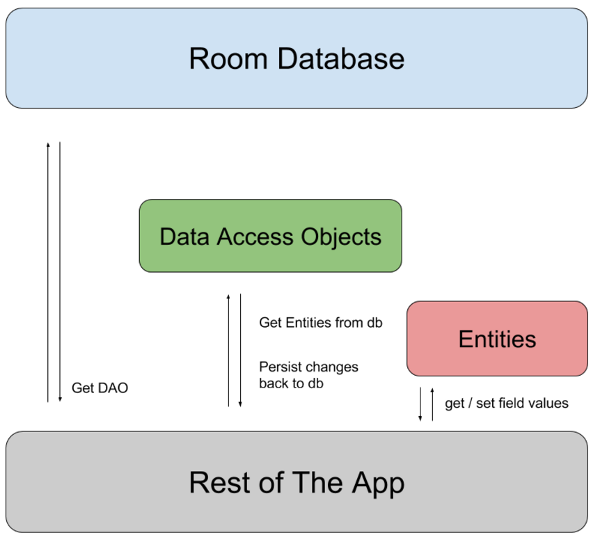
\includegraphics[width=.8\textwidth]{assets/room_architecture}
	\caption[Room architecture]{Room architecture\cite{android:training:jetpack:room}}
	\label{room_architecture_img}
\end{center}
\end{figure}

The Entity\cite{android:training:jetpack:room:entities} is the model that we are saving in the database. The advantage here is that we do not need to build a model and a separate table, we can just annotate our model with \mintinline{kotlin}{@Entity} and other annotations to define the database table automatically.

For example, a \verb+User+ entity is just a data class in Kotlin:
\begin{code}
\kotlincode{assets/code/kotlin/userEntity.kt}
\caption{A Room User entity}	
\end{code}



Then, we have to write a \gls{dao}\cite{android:training:jetpack:room:dao} interface for the entity to create methods to interact with the entity in the database. There are methods automatically created for us, such as insertion and deletion of single entries. Queries returning elements from the database have to be written in \gls{sql}, but the \gls{ide} provides completion and there is compile time check of \gls{sql} syntax with table and column names. Finally, we can easily ask for returning LiveData for a query simply by specifying in the signature function.

For example, for the \verb+User+ \gls{dao}, we can just wrap all the return values from \verb+SELECT+ queries in \verb+LiveData+ and we will get them in that format:
\begin{code}
\kotlincode{assets/code/kotlin/userDao.kt}
\caption{A Room User DAO definition}	
\end{code}


Finally, you can then write the Database\cite{android:training:jetpack:room:db} class by providing an array of the entities and creating an abstract fun to retrieve each \gls{dao}. It is also suggested to make the Database class a Singleton\cite{android:training:jetpack:room}:
\begin{code}
\kotlincode{assets/code/kotlin/userDb.kt}
\caption{Setting up a Room Database}	
\end{code}


%%TODO do we talk about typeconverters?
\paragraph{ViewModel}
The ViewModel\cite{android:doc:viewmodel} bridges the gap between the data and the UI data in a lifecycle aware way. As opposed to storing data in variables in an Activity, data in a ViewModel will remain persistent when configuration changes, for example when rotating the screen.

It is suggested to also implement a Repository behind the ViewModel to abstract the source of the data, database or network for example. In the Repository, we can also write wrapper around insertion tasks to run them on separate threads because you can't run database operations on the main thread\footnote{Queries returning LiveData already run on a background thread, due to the LiveData returning value asynchronously}.

The user Repository and ViewModel look like this:
\begin{code}
\kotlincode{assets/code/kotlin/userViewModel.kt}
\caption{User repository and ViewModel definition} 	
\end{code}


\paragraph{LiveData}
\label{livedata}
LiveData\cite{android:doc:jetpack:livedata} is an observable holder class that allows to react to data changes. The advantage of LiveData is that it is lifecycle aware, so you can observe the data by passing it an Activity or Fragment and will pause and resume accordingly when the Activity is paused or resumed. Otherwise, we could try refreshing the UI when the data changes and if the Activity is not in the foreground, the application would crash. LiveData allows us to always update our UI with the latest data, for example data from a Room Database.\\

You can just call the \verb+observe+ method on a LiveData instance and pass a lifecycle component, in this case a Fragment and an Observer callback to handle the data.
\begin{code}
\kotlincode{assets/code/kotlin/userLiveData.kt}
\caption{Observing LiveData on Android}	
\end{code}


\paragraph{Putting everything together}
When putting everything together\cite{android:codelab:room}, we can see the interactions in figure \ref{viewmodel_interactions_img} with the ViewModel providing LiveData to the Fragment or Activity that can update the UI by observing it. The \verb+ViewModelProviders.of()+ is used to retrieve the requested ViewModel from the system.
\begin{figure}[H]
\begin{center}
	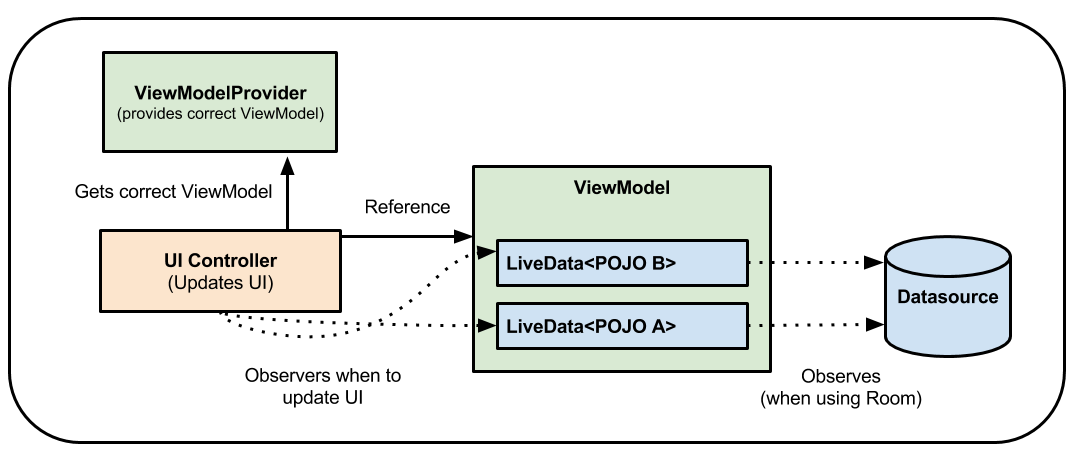
\includegraphics[width=.8\textwidth]{assets/viewmodel}
	\caption[View model interactions]{View model interactions\cite{android:doc:viewmodel}}
	\label{viewmodel_interactions_img}
\end{center}
\end{figure}

If for example, we couple this with a RecyclerView and decide to get a list of all users from the database to display it, it gives us the following code:
\begin{code}
\kotlincode{assets/code/kotlin/userRoomComplete.kt}
\caption{Using Room, ViewModels and LiveData to display a list of Users}	
\end{code}


\subsubsection{Work Manager - Background jobs}
WorkManager\cite{android:doc:jetpack:work_manager} allows running background asynchronous tasks, for example downloading data from a backend. The advantage behind using WorkManager is that it will choose the correct implementation depending on the Android version it is running on and the available APIs. It will also adapt to the state of the app, running or not. Android has several background work mechanisms depending on the platform and WorkManager provides a way to avoid choosing one of them.\\

To use WorkManager, you have to create a class that extends the \verb+Worker+ class and implement the method \mintinline[breaklines]{kotlin}{fun doWork(): Result}. This function returns a \verb+Worker.Result+ that can be either a success, a failure or a request to retry. You have access to the application context from this class, so you can save data to a database for example or access SharedPreferences.\\

For example, if we want to write a Worker to retrieve a \verb+User+ from the backend, we can do it this way\cite{android:codelab:work_manager}:
\begin{code}
\kotlincode{assets/code/kotlin/workmanager.kt}
\caption{Simple WorkManager Worker implementation}	
\end{code}
\subsubsection{Navigation}
\label{jetpack_navigation}
Navigation inside an application has always been more complicated on Android than on iOS. For example, all Android devices have a "back" button in the \gls{os} navigation bar at the bottom and the Android guidelines also define an "up" button in the application toolbar that most applications implement. The "up" button looks exactly like the "back" button and most user think it does exactly the same thing but that is not the case (see figure \ref{twitter_up_back_img}). The "up" button should move to the hierarchical parent screen of the current screen, so let's say that we are inside a messaging conversation, the "up" button brings us back to the conversations list. Pressing the "back" button brings us back to the screen that was used before arriving to the current screen. For example, if we were browsing the web and clicked on a notification that brought us to the messaging conversation, pressing "back" brings us back to the web browser.\\

The problem here is that when deep linking in a screen directly, for example from a notification, we had to fill in ourselves in the backstack the hierarchical parents so that the "up" button behaved correctly. Some apps do not implement this in the correct way and by default the "up" button destroys the Activity or acts as a "back" button. This does not guarantee an excepted behaviour of those buttons for the user.\\

\begin{figure}[H]
\begin{center}
	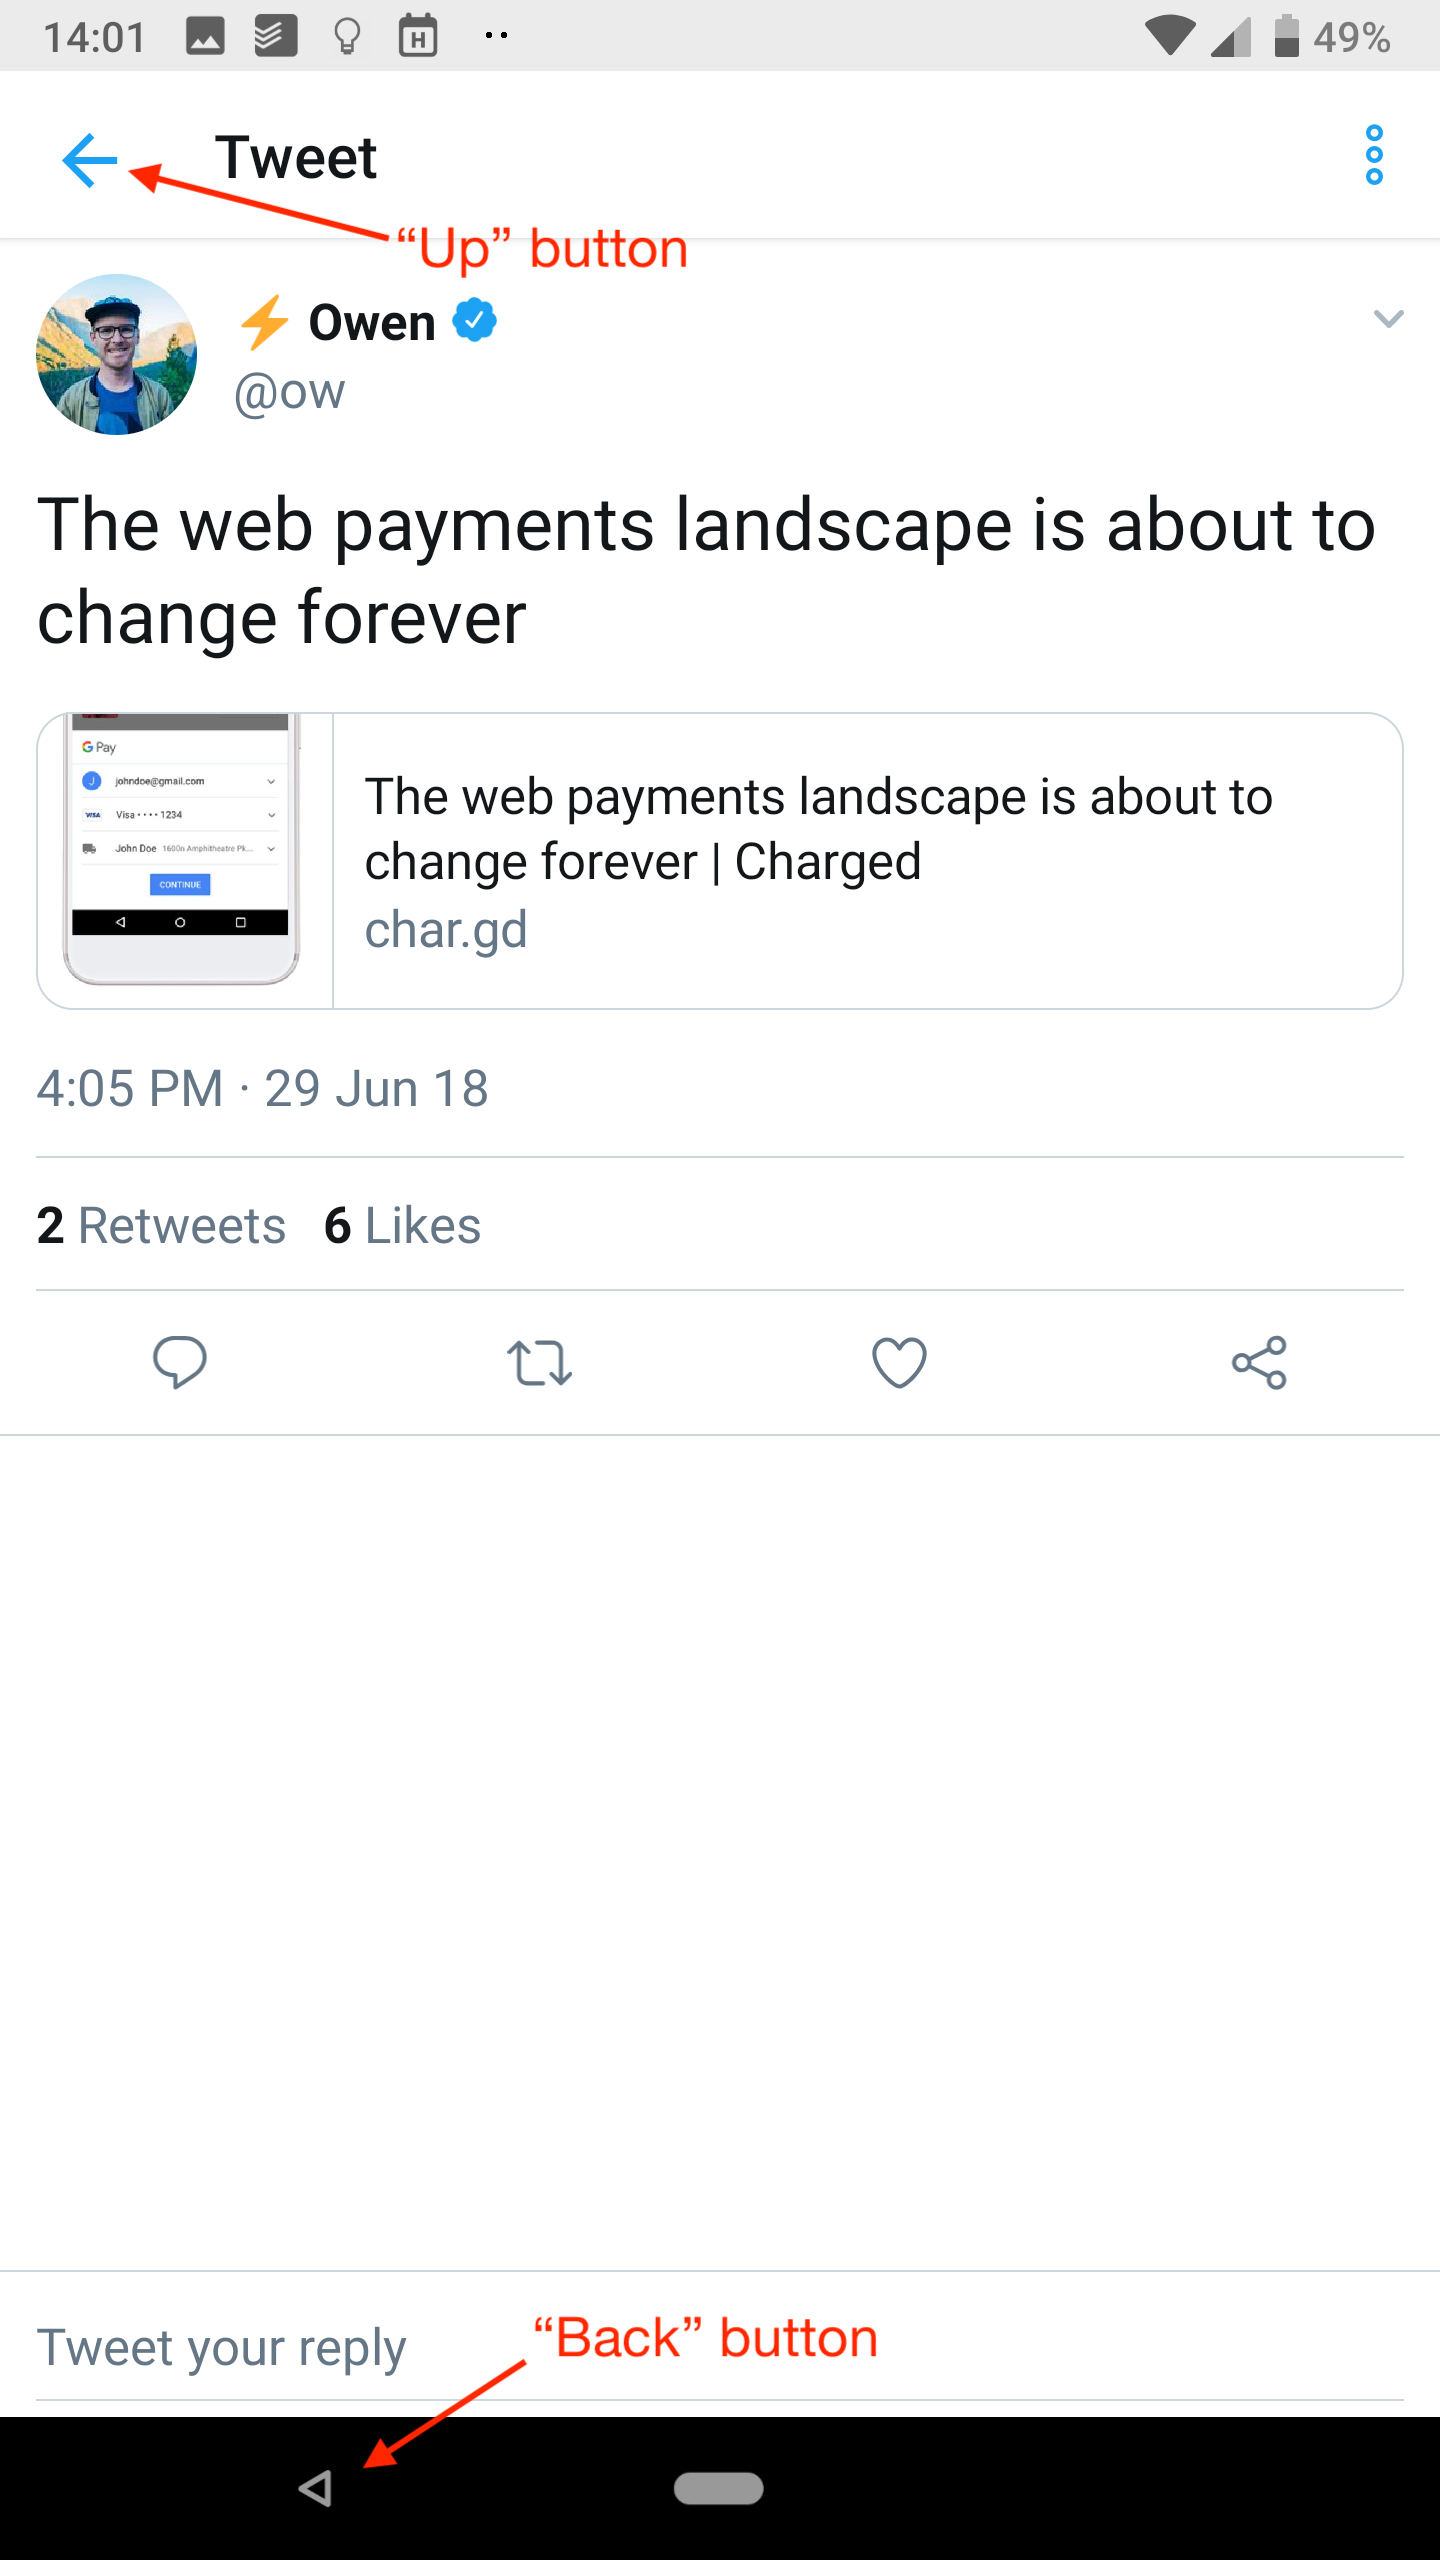
\includegraphics[width=.5\textwidth]{assets/twitter_app_up_back}
	\caption[Up and Back buttons in Twitter app]{In the Twitter app, the "up" and "back" buttons have the correct behaviour, "up" brings you back to your timeline and "back" to the precedent screen}
	\label{twitter_up_back_img}
\end{center}
\end{figure}

What Google aims to do with the new Navigation Architecture Component\cite{android:doc:jetpack:navigation} is simplifying the life of developers and the implementation of complex navigations with clear hierarchy of screen and automatic handling of the backstack\cite{android:video:io2018:navigation}. It also aims to move away from writing an Activity for every screen and instead handling navigation by switching Fragments inside the same Activity. It is introducing a new library to handle Navigation as well as a graphical editor to more easily setup relations between screens\footnote{The graphical navigation editor is available as an experimental feature in Android Studio 3.2 (Beta at the time of this writing). You can use the navigation feature in XML as well}.\\


\paragraph{Visual editor}
As we can see in figure \ref{navigation_editor}, we have a view of all our screens and the links between them. If a link exists between two screens, it means we can call the corresponding method to create a transition between the two screens and pass it to the Navigation Controller.\\

\begin{figure}[H]
\begin{center}
	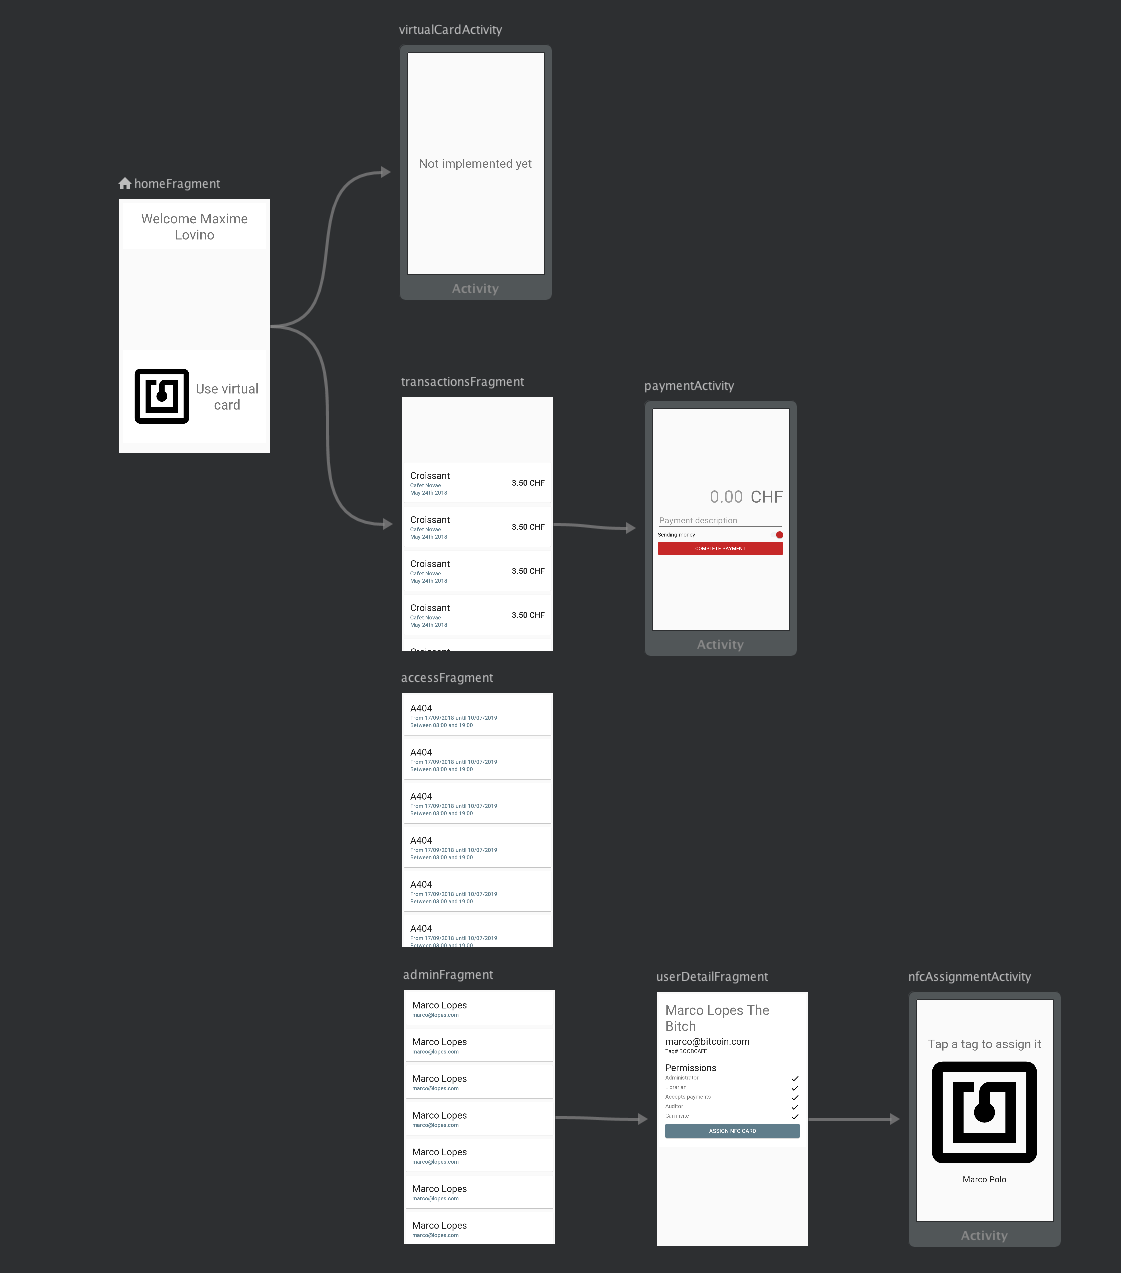
\includegraphics[width=.8\textwidth]{assets/navEditor}
	\caption[Navigation visual editor]{The new Navigation visual editor}
	\label{navigation_editor}
\end{center}
\end{figure}

\paragraph{Integrating with Bottom Navigation View}
In most cases, what you want do is integrate the top level screens with a Navigation UI element, for example a Bottom Navigation View\cite{android:doc:material:bottom_nav}. To do this, first of all you need to define the menu for the bottom navigation by specifying an ID for each entry in your Bottom Navigation menu (see source code \ref{bottom_nav_menu}). Then you have to create a Fragment in the layout of the Activity, link it to the Navigation XML file and specify that it is a \verb+NavHostFragment+ (see source code \ref{Activity_nav_host}).
\begin{code}
	\xmlcode{assets/code/xml/bottomNav.xml}
	\caption{Menu defining the bottom navigation}
	\label{bottom_nav_menu}
\end{code}

\begin{code}
	\xmlcode{assets/code/xml/activityNavHost.xml}
	\caption{The container Fragment to define that will host the Navigation selected screen}
	\label{Activity_nav_host}
\end{code}

Afterwards, when populating the Navigation using the visual editor, use the same ID used in the menu on the corresponding screen in the navigation. Finally, when created the Activity, you can find the Navigation Controller which, on Kotlin, integrates a method to directly link to the Bottom Navigation View. This will link active states on each button corresponding to the active screen and enable switching between the screens with the Bottom Navigation (see source code \ref{linking_nav}).

\begin{code}
	\kotlincode{assets/code/kotlin/setupBottomNav.kt}
	\caption{Linking Bottom Navigation View with Navigation Controller}
	\label{linking_nav}
\end{code}
\paragraph{Safe arguments}
Another pain point that the Navigation Controller solves is the passing of arguments between screens. Until now, if you wanted to pass arguments to another screen, you had to add them to the \verb+Intent+ bundle that you were starting or in the Fragment constructor. These were just key/value pairs and there was no verification that the arguments were correctly passed.\\

In the Navigation Controller, you can define input arguments for the screen. For example, a screen presenting the details for a \verb+User+ can take the ID of the \verb+User+ as a \verb+String+ argument. Then, if we want to navigate to that screen, we have to pass the corresponding argument otherwise the application will not compile. The arguments are type-checked as well. \\

When setting up a transition between two screens, you give it an ID (see figure \ref{transition_nav}) and then the library will generate a \verb+<sourceScreenName>Directions+ class that contains methods for each outgoing transitions available from the \verb+sourceScreenName+. These methods take the required arguments as parameters and create a \verb+NavDirection+ instance that can be passed to the Navigation Controller.
\begin{figure}[H]
\begin{center}
	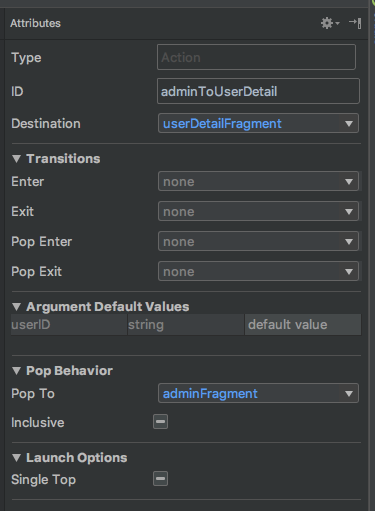
\includegraphics[width=.5\textwidth]{assets/transition_nav}
	\caption[Transition between screens]{Setting up a transition between screens in Navigation Editor}
	\label{transition_nav}
\end{center}
\end{figure}

For example, if we want to navigate from a users list (\verb+AdminFragment+) to the user detail screen(\verb+UserDetailFragment+), we can use the following code:
\begin{code}
	\kotlincode{assets/code/kotlin/navExampleArgs.kt}
	\caption{Navigating from a screen to another by passing arguments}
\end{code}

Then in the destination screen, we can unwrap the passed arguments by using the generated \verb+<destinationScreenName>Args+ class like this:
\begin{code}
	\kotlincode{assets/code/kotlin/navExampleArgsReceiving.kt}
	\caption{Receiving input arguments when navigating}
\end{code}

\section{Angular 6}
\label{angular_chapter}
%%TODO should we talk about the main module file?
%%TODO talk about ng serve
%%TODO talk about exporting and running with Nginx

Angular\cite{angular:website} is a web application frontend framework. It is opne source and developed actively on GitHub\cite{github:angular} by the Angular team at Google and other individual contributors. Angular 1 was originally built in JavaScript (now AngularJS) and has now been replaced since version 2 by a new version of Angular (commonly called Angular 2, even though version 6 is out) built in TypeScript. \\

The main advantages of using a frontend framework are modularity and a clear code structure compared to not using any frameworks. \\

Angular provides a \gls{cli} tool called \emph{Angular CLI} and used with the \verb+ng+ command that helps initialising and updating projects. The \gls{cli} also handles code generation, for example when creating a component, it will create all required files and register the component in the application module, more on that later. All Angular \gls{cli} commands should be run from the root directory of the Angular project. \\

Angular projects are usually installed and run through \gls{npm}, although Yarn can be used as well.
\subsection{Single-page webapp}
Angular is used to build web applications, as opposed to websites. While for most users the differences between these two are not noticeable, web applications behave more like native applications and allow interactions from the user.\\

Often, web applications are single-page applications. That does not mean that the application only has a single screen but it means that you only need to load one page and then all other navigation is handled by the page itself.

In the case of Angular web applications, you only have one entry point page and then the internal Angular Router in the web application will take care of the rest, without needing to load new pages or refresh the browser.
\subsection{Architecture of an Angular Application}
An Angular application is built around Modules (called \emph{NgModules})\cite{angular:doc:modules} that contain Components and Services. Each application has at least one root Module, called the AppModule. You can create additional Modules to group related Services and Components together and then import these Modules inside the AppModule.
\begin{figure}[H]
\begin{center}
	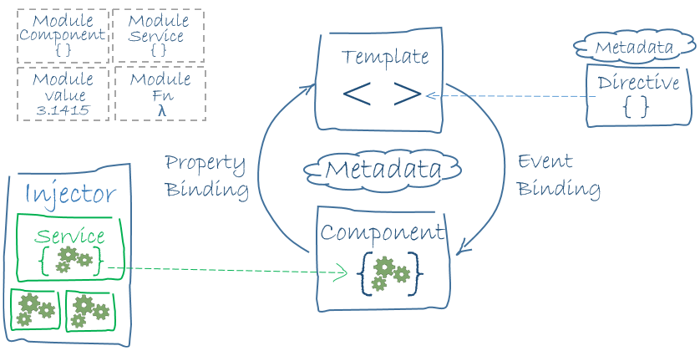
\includegraphics[width=.8\textwidth]{assets/angular_architecture}
	\caption[Architecture of an Angular application]{Architecture of an Angular application\cite{angular:ref:architecture}}
\end{center}
\end{figure}
\subsubsection{Folder structure}
When initiating a new project with the Angular \gls{cli}, it will setup the default folder structure and a set of initial files to work with.

To create a new "demo" project, you can use the following command:
\begin{code}
	\begin{shell}
ng new demo
	\end{shell}
	\caption{Command to create a new Angular project}
\end{code}
And it will present you with this starting architecture:
\dirtree{%
.1 demo. 
.2 README.md.
.2 angular.json.
.2 e2e.
.3 protractor.conf.js.
.3 src.
.4 app.e2e-spec.ts.
.4 app.po.ts.
.3 tsconfig.e2e.json.
.2 node\_modules/.
.2 package-lock.json.
.2 package.json.
.2 src.
.3 app.
.4 app.component.css.
.4 app.component.html.
.4 app.component.spec.ts.
.4 app.component.ts.
.4 app.module.ts.
.3 assets.
.3 browserslist.
.3 environments.
.4 environment.prod.ts.
.4 environment.ts.
.3 favicon.ico.
.3 index.html.
.3 karma.conf.js.
.3 main.ts.
.3 polyfills.ts.
.3 styles.css.
.3 test.ts.
.3 tsconfig.app.json.
.3 tsconfig.spec.json.
.3 tslint.json.
.2 tsconfig.json.
.2 tslint.json.
}

The main application files are contained in the \verb+src/+ directory.The \verb+src/app/+ contains the AppModule and an initial App Component created for us. The main \verb+index.html+ template file and the main stylesheet are also created. The \verb+e2e+ is used for testing using the \verb+e2e+ testing framework. The \verb+tslint.json+ files provides a configuration and code conventions for us to run TSLint with. The \verb+tsconfig.json+ contains the TypeScript compiler configuration for the project.
\paragraph{angular.json}
This is the main configuration file for the Angular project. It contains directory and path configurations for the project as well as options on whether to use CSS or SASS for stylesheets. It also contains the configuration about hostnames and ports to use as well as SSL configuration for the built-in development web server.

\paragraph{package.json}
As in all \gls{npm} projects, this files contains all the \gls{npm} module dependencies of our application with their respective version as well as define commands to be run with the \verb+npm run+ command. To update our application dependencies, for example when a new Angular version comes out, we can use the Angular \gls{cli} with the command and then follow the on-screen instructions:
\begin{code}
	\begin{shell}
ng update
	\end{shell}
	\caption{Command to check for available Angular updates}
\end{code}

When updating dependencies, the Angular \gls{cli} will update the \verb+package.json+ file with the new packages versions and then install the new dependencies.

\subsubsection{Components}
A Component\cite{angular:doc:components} is used to control a subset of a view in the application. By creating small single-purpose Components, for example a Component showing only a User detail, you can easily reuse Components in multiple views. \\

To generate a new Component using the Angular \gls{cli}, you can use the following command:
\begin{code}
	\begin{shell}
ng generate component <componentName>
	\end{shell}
	\caption{Command to generate a new Angular Component}
\end{code}

This will create a folder containing four Component files:
\begin{itemize}
	\item A stylesheet file (CSS or SASS depending on the project configuration)
	\item A HTML template file
	\item A TypeScript file for the logic
	\item A specification TypeScript file (used by the compiler and autocomplete tools for typings)
\end{itemize}

If we generate a Users component for example, we can use the command:
\begin{code}
	\begin{shell}
ng generate component users
	\end{shell}
	\caption{Command to generate a Users Component}
\end{code}
This will generate the following hierarchy in the \verb+src/app/+ folder:
\dirtree{%
.1 users. 
.2 users.component.html. 
.2 users.component.scss. 
.2 users.component.spec.ts. 
.2 users.component.ts. 
}

The content of the TypeScript file of the component is the following:
\begin{code}
	\tscode{assets/code/typescript/defaultComponent.ts}
	\caption{Empty Component TypeScript file}
	\label{component_code}
\end{code}

Here in source code \ref{component_code}, we can see the Component metadata. The \verb+templateUrl+ and \verb+styleUrls+ are pretty self-explanatory, they reference the corresponding two other files and should keep their default value. The \verb+selector+ is the value of the HTML selector you can use in other HTML templates to insert your component. So, if we have another higher level, for example an homepage and we want to insert our users component, we can insert it using this selector (see source code \ref{integrating_component_selector}). The selector by convention should start with \verb+app-*+ in order to avoid clashing with HTML default selectors.
\begin{code}
	\htmlcode{assets/code/html/integratingComponent.html}
	\caption{Integrating Component in template with selector}
	\label{integrating_component_selector}
\end{code}

Afterwards, you can create methods and properties in the Component TypeScript file that can then be called and mapped to the templates. 
\paragraph{Templates}
Templates\cite{angular:doc:templates} are just HTML files on the surface with additional features inherent to Angular. One of these is interpolation of template expressions. If you have a public property in the TypeScript file or you want to display the output of TypeScript code, you can do so in the Template by wrapping it in curly braces.

For example, let's say we had a \verb+name+ property to the User component and we want to display it in the template, we can do so by using the \verb+{{name}}+ text in our template.\\

Moreover, we can define HTML elements properties with TypeScript code.For example, if we want to disable an input in HTML, we can use:
\begin{code}
\begin{inlinehtml}
<input type="text" disabled>
\end{inlinehtml}
\caption{Static disabling input in HTML}	
\end{code}
Now, if we want to have a boolean property in the TypeScript file that decides if the input is enabled or disabled, we can do this using the brackets notation \verb+[]+. This is useful for example if we want to enable according to a form validity. By putting the \verb+disabled+ properties in square brackets, the compiler will interpret the text passed as TypeScript code, this is called property binding. So if we have a boolean \verb+formValid+ that states if the input is enabled or not, we can use:
\begin{code}
\begin{inlinehtml}
<input type="text" [disabled]="formValid">
\end{inlinehtml}
\caption{Enabling/disabling input in HTML with TypeScript}	
\end{code}

Finally, we have access to control flow inside the Template. This is useful for example if we want to display all elements from a list. Let's take a property \verb+users+ in our template that is a list of User with each User having a name and we want to display each User has a bulletpoint with a simple message to tell that there are no users if the list is empty. We can use \verb+ngFor+ and \verb+ngIf+ control flow operators to accomplish this:
\begin{code}
	\htmlcode{assets/code/html/controlFlowTemplate.html}
	\caption{Control flow inside Angular Templates}
\end{code}
We can also use \verb+ng-container+ and \verb+ng-template+ to more visually separate our two branches with an \verb+if-else+ in the template:
\begin{code}
	\htmlcode{assets/code/html/controlFlowTemplateAlt.html}
	\caption{Alternative control flow inside Angular Templates}
\end{code}
\paragraph{Communication between components - Event emission}
\label{communication_components}
Communication is useful between Components because often you have a parent Component handling a whole screen with children Components inside the view. In this case, the parent component can act as an intermediary in the communication between two children Components (see figure \ref{communication_figure}). \\

\begin{figure}[H]
\begin{center}
	
\includegraphics[width=.8\textwidth]{assets/componentsComm}
	\caption{Event emission and communication between components}
	\label{communication_figure}
\end{center}
\end{figure}

The parent Component can have properties for each child Component by selecting it as a property using the \verb+@ViewChild()+ annotation. As an example, we can take a \verb+UsersComponent+ which integrate a \verb+CreateUserComponent+ and a \verb+UserTableComponent+. The goal here is to refresh the table when a new User is created. To accomplish this, the \verb+CreateUserComponent+ must emit an event when a new User is created and the parent Component will catch it and call a method on the table to refresh it. \\

From the parent component point of view, it looks like this:
\begin{code}
	\htmlcode{assets/code/html/usersInteractionParent.html}
	\tscode{assets/code/typescript/usersInteractionParent.ts}
	\caption{Template and logic files of the parent component}
	\label{parent_component_files}
\end{code}
When looking at source code \ref{parent_component_files} Template file, we can see \verb+(created)+ that is assigned to a function call and passing \verb+$event+ to that function. This is called event binding.\\

Inside the \verb+CreateUserComponent+, the \verb+created+ property is defined as an \mintinline[breaklines]{ts}{@Output() created = new EventEmitter<boolean>();}. With this event emitter, we can call the method \verb+emit()+ on it to emit a value of the specified type, in our case \verb+boolean+. The \verb+$event+ passed to the function call in the parent component is the value passed at the emission of the event.

From there, we can just call any public method in the table component, in this case \verb+refreshData()+.

\paragraph{Communication between components - Input parameters}
Finally, you can also have parametric Components. These Components can be integrated inside other Components through their selector but you also have to specify a set of inputs for the Component. In the Component, these inputs are properties with \verb+@Input()+. \\

For example, if we have a Component displaying a single User, this Component would take the User to display as a parameter. So in the Component, we can write the User property like this and it will behave like any other property:
\begin{code}
	\begin{inlinets}
@Input() user: User;
	\end{inlinets}
	\caption{Input property in Component}
\end{code}

To set this property when integrating the Component in a parent Component, we can simply specify it like this:
\begin{code}
	\begin{inlinehtml}
<app-user-entry [user]="User('toto')"></app-user-entry>
	\end{inlinehtml}
	\caption{Setting an input property in Component}
\end{code}
\subsubsection{Services}
Services\cite{angular:doc:services} are a broader category than Component and can be seen as code that is not directly related to user interaction or user experience. Services are also often shared and used by different Components using Dependency Injection\cite{angular:doc:dependency_injection} (see \ref{dependency_injection}). Services can contain methods to manage and save data, to fetch data from a server, validate inputs. All those methods can then be called by all Components simply by injecting the Service. You can use other Services inside a Service simply by injecting them in the Service (see \ref{dependency_injection}).\\

To generate a new Service, you can use the Angular \gls{cli}:
\begin{code}
\begin{shell}
ng generate service <serviceName>
\end{shell}
	\caption{Creating a new Service using the Angular \gls{cli}}
\end{code}
This will create a TypeScript file and a specification file in the \verb+src/app/+ directory. 
\paragraph{Dependency injection}
\label{dependency_injection}
When you create a Service using the Angular \gls{cli}, it is annotated with the \verb+@Injectable(...)+ annotation. You then have to import it in the AppModule file and add it to the \verb+providers+ array of the Module. From then on, you can use it in any other Service or Component simply by adding it to the Component or Service constructor. \\

For example, if we have a \verb+UserService+ that we want to use in our \verb+CreateUserComponent+, we can just use the following code to access the Service inside the Component:
\begin{code}
	\tscode{assets/code/typescript/injectingService.ts}
	\caption{Injecting a Service inside a Component}
\end{code}
\subsubsection{Routing}
Routing\cite{angular:doc:router} inside the application is handled by the Angular Router. Even though our web application is a single-page application from the browser point of view, it is important to use a Router and not just load and unload content in a single URL. This enables for example deep linking to directly access a page of the application. \\

To generate a Router, you need to generate a new Module to contain the Router. To do so, you can use the Angular \gls{cli}:
\begin{code}
	\begin{shell}
ng generate module app-routing --flat --module=app
	\end{shell}
	\caption{Generating a routing module with the Angular \gls{cli}}
	\label{router_gen}
\end{code}
In source code \ref{router_gen}, the \verb+--flat+ parameter tells the \gls{cli} to put the new Module at the root of the \verb+src/app/+ without creating a separate folder and the \verb+--module=app+ parameter imports the newly created Module in the AppModule. \\

Then, we need to create the Router inside our Module. To do this, first you need to import the \verb+RouterModule+ and \verb+Routes+ class from Angular:
\begin{code}
	\begin{inlinets}
import { RouterModule, Routes } from '@angular/router';
	\end{inlinets}
	\caption{Importing required elements for Routing}
\end{code}

Then, we have to define the routes. Routes are defined as an array of Route, for each entry, we can specify several properties, such as a path, a redirection, a set of Guards (see \ref{guards}) to pass to activate the Route and a Component to load. There are more properties, but these are the main ones and we will not dive further into the others. \\

The finality of each Route is to load a Component on screen, be it directly or through a redirection to another Route that loads a Component. \\

For example, if we have a \verb+HomePageComponent+ to load for the homepage and a \verb+UsersComponent+ to load for the \verb+/users+ and we want to redirect everything else to the homepage, we can use the following Routes:
\begin{code}
	\tscode{assets/code/typescript/simpleRoutes.ts}
	\caption{Two pages Routes setup in Angular}
	\label{simple_routes}
\end{code}

Then, in the Module that we created for routing, after defining the routes, we have to link the \verb+RouterModule+ with the Routes and export the Router as part of our Module:
\begin{code}
	\tscode{assets/code/typescript/exportingRouter.ts}
	\caption{Setting up Router and exporting it in Angular}
\end{code}

Finally, we can also create a hierarchy of Routes by adding children to Route entries. This is particularly useful if we want to protect a set of routes (admin routes for example) behind a Guard (see \ref{guards}).If we take the example from source code \ref{simple_routes} and want to add a \verb+/users/create+ create under the \verb+/users+, we can refactor it this way:
\begin{code}
	\tscode{assets/code/typescript/nestedRoutes.ts}
	\caption{Nested Routes in Angular}
	\label{nested_routes}
\end{code}

\paragraph{Router outlet}
Finally, to display the routed component in our page, we have to provide a Router Outlet. The Router Outlet is often inserted as the only element directly in the main \verb+index.html+ file but can also be inserted in a more complex layout or in another Component. The Router will attach itself to the first encountered Router Outlet from a hierarchical standpoint.\\

To insert the Router outlet in a template, you can use its selector:
\begin{code}
\begin{inlinehtml}
<router-outlet></router-outlet>
\end{inlinehtml}
	\caption{Using a Router Outlet in Angular}
\end{code}
\paragraph{Guards}
\label{guards}
Finally, another important part of Routing are Guards. By default, anyone can navigate to all the Routes in the application but in many real use cases, you have to be logged in to access specific sections of an application or even have special permissions. Guards allow to perform checks before activating a Route and multiple Guards can also be chained to enable a Route activation. \\

The most basic will return a \verb+Boolean+ to specify if the user can pass the Guard or not. Inside the guard, you can also access the Router by Dependency Injection to provide a redirection in case the check does not pass for example. \\

As an example, we can take a look at one of the most common Guard used. This Guard is used to protect a Route only available to logged-in users and will redirect to the \verb+/login+ page if the user is not logged-in.\\

First of all, we can generate the Guard that we're going to call the \verb+AuthGuard+ using the Angular \gls{cli}, we have to add it to the \verb+providers+ array in the AppModule as well:
\begin{code}
	\begin{shell}
ng generate guard auth
	\end{shell}
	\caption{Generating a guard using Angular \gls{cli}}
\end{code}
Then, we can add the Guard to our Route. If we take the Routes from source code \ref{simple_routes} and add a \verb+/login+ Route, we will then protect all other Routes behind the guard:
\begin{code}
	\tscode{assets/code/typescript/simpleRoutesGuard.ts}
	\caption{Routes protected by a Guard}
\end{code}

Then we have to write the logic of the Guard itself with the redirection. To do so, we have a service that will returns an \verb+Observable+ that specifies if the user is logged-in (more info on \verb+Observable+ operators \verb+pipe+ and \verb+tap+ in section \ref{observables}) and we are gonna return the logged-in value to the guard and redirect if it's false:
\begin{code}
	\tscode{assets/code/typescript/guard.ts}
	\caption{Guard redirecting not logged-in users to login page}
	\label{authGuard}
\end{code}
\subsection{RxJS - Observables}
\label{observables}
RxJS Observables\cite{angular:doc:observables} are similar in concept to LiveData on Android (see section \ref{livedata}). The idea behind Observable is to return a value that can change over time and on which you can "listen" for new changes and update the UI accordingly for example. It is used for changing data, for example when subscribing to breakpoint changes in browser window (resizing the window) or for data that is not yet available and is being loaded asynchronously from memory or another server. \\

In most project, RxJS Observables are mainly used by the Angular HTTPClient\cite{angular:doc:http}. Since HTTP requests are asynchronous, when making a request the client returns an Observable on which you can subscribe to get the parsed result once it comes back from the server.\\

\subsubsection{The HTTP Client}
The HTTP Client is used to retrieve \gls{json} Data from a backend \gls{api}. It returns an Observable of the data already parsed to the correct type. Its recommended to use the HTTP Client in a Service and you can access it by Dependency Injection in any Service.\\

If we want to retrieve the list of all users from the backend, we have to create a \verb+User+ TypeScript class in our Angular project to match the data returned from the backend. Then we can simply use the HTTP Client to make a request and it will return an \verb+Observable<User[]>+:
\begin{code}
	\tscode{assets/code/typescript/httpUsers.ts}
	\caption{Using the HTTP Client to retrieve data}
\end{code}

Then, when calling this method from a Component for example, we can \verb+subscribe+ to the Observable and get two branches: one if data is available and another if an error happens, we can supply functions for each case:
\begin{code}
	\tscode{assets/code/typescript/gettingObservable.ts}
	\caption{Subscribing to data from an Observable}
\end{code}
\subsubsection{Pipe and other operators}
Sometimes it can be useful to handle the data of an Observable before the subscribers are notified of new data. This is done using the \verb+pipe+ operator. When returning an Observable, you can append a call to \verb+pipe+ at the end of it and insert operations that will be run as part of the Observable before it triggers the subscribers. These operations are function calls that take a \verb+function(data)+ as parameter. \\

One of the operations that can be run is the \verb+tap+ operation. This operation does not make any change to the data being sent to the subscribers but allows to use it before sending it untouched. For example, it is used in the the \verb+AuthGuard+ presented before (source code \ref{authGuard}) to access the returned data so that it can redirect to the \verb+/login+ page if the user was not logged in. Basically, we pass the value to the function caller, but we can use it too when it comes back.\\

Another useful operator is the \verb+map+ operator. This is used to transform data before it triggers the subscribers. It will return an Observable of the type of the returned value in the map function. For example, if we need to return an \verb+Observable<boolean>+ to say if the user is logged-in and we have a \verb+getToken+ function that sends us the authentication token or \verb+null+ if no user is logged in, we can use the \verb+map+ operator to transform our \verb+Observable<String>+ in an \verb+Observable<boolean>+. We can do this by using the following code:
\begin{code}
\tscode{assets/code/typescript/observableMap.ts}
	\caption{Transforming an Observable using the map operator}
\end{code}
\subsection{TypeScript}
TypeScript\cite{github:typescript} is an open source language developed by Microsoft. It adds optional static typing and classes to JavaScript as well as implementing its own module import syntax. TypeScript files can be "compiled" to JavaScript to be used on the web or on the server-side using Node.JS for example. TypeScript is regarded by Microsoft and others as the way to build large scale JavaScript application thanks to the ease of mind provided by statically typed languages. \\

TypeScript also includes the ability to write definition files to add typing information to existing JavaScript code to provide completion in code editor as well as compile-time check when using third-party libraries. \\

The whole static typing logic is checked when "compiling" (actually transpiling) to JavaScript. The generated JavaScript files are plain JavaScript files and can be configured to use ES6 syntax or earlier by providing compatibility code for older JavaScript standards. \\

The syntax of TypeScript is similar to JavaScript with the main addition being the ability to specify the type of a variable or the return type of a method by appending \verb+:<type>+ to its declaration, for example:
\begin{code}
	\begin{inlinets}
let age: number = 10;
	\end{inlinets}
	\caption{Defining the type of a variable in TypeScript}
\end{code}
\subsection{Angular Material}
Angular Material\cite{angular:material:website} is an open source\cite{github:angular:material} Components library built by the Angular team to be used with Angular. The library provides Angular Components that follow the Material Design Language\cite{material:website} used by Google on Android and the web.\\

Contrary to a simple stylesheet library, Angular Material provides Angular Components that incorporate their own logic and not only look but also behave according to the Material Design specification. These Components range from side navigation drawers to tables complete with sorting and filtering. It also provides extensive theming capabilities with the ability to change theme colors globally or on a component basis. \\

Finally, a Component Development Kit is provided to simplify building custom Material-inspired Components.
\section{NoSQL Database - MongoDB}
%%TODO add wikipedia ref for noSQL, mongo from wikipedia
NoSQL databases\cite{wiki:nosql} have existed for a long time, since the late 1960s but only recently have they started become more and more popular, due to the advent of Big Data and real-time applications. While most people believe that NoSQL databases are named this way because they are \emph{NOT} \gls{sql}, it actually should mean \emph{Not-Only \gls{sql}} as some NoSQL system support \gls{sql}-like syntaxes for queries. \\

According to the \emph{CAP Theorem}\cite{wiki:cap_theorem}, it is impossible for a distributed data store to provide more than two out of: Consistency, Availability and Partition tolerance. NoSQL stores often compromises some consistency in favour of better availability and speed as well as simplified scaling. \\ 

NoSQL databases do not use the same data structures as \gls{sql} databases and there are several categories of NoSQL databases classified by the data structures they use. Some of these categories are:
\begin{itemize}
	\item Key-Value store
	\item Document store
	\item Object database
	\item Graph databases
\end{itemize}

MongoDB\cite{wiki:mongo} is a document-oriented database\cite{wiki:document_oriented_db} launched in 2007 that store \gls{json}-like documents in collections. It is currently one of the most used NoSQL data stores. The document would be the equivalent to a row in \gls{sql} and the collection is the equivalent to a table.

\subsection{Schemas}
By default, MongoDB does not impose a strict Schema inside a collection, meaning all documents inside the collection can have a different structure. While it is not a best practice, it provides flexibility when the project is still in development phase because you can modify the schema and save new documents with newly added or modified fields while already present keep their structure. When running in production, the schema should be strict in all collections. \\
\subsubsection{How to handle references}
\label{mongo_references}
Often documents you save in the database will have a relation with other documents from another schema. These relations would be stored in a \gls{sql} Database as a Foreign Key linked to the Primary Key of the entry we want to reference. In MongoDB, there are three solutions to handle references depending on the number of references that are necessary from one document to another. You should think from the beginning about the maximum number of references you can have between two documents before choosing one of three references design. The limitations of the designs come from the maximum size of a MongoDB document, that is capped at 16Mb, and if you need to update referenced documents often. \\

To illustrate the three options, we are gonna take an example where we people and cars. There is one schema for a person and one schema for a car and a person can have multiple cars but a car is only owned by a single person. \\

The first option to store this information is to embed the car documents in the person document\cite{mongo:doc:refs:embeddingRefs}. We don't need to have a car collection, we can just store in the person document an array of cars. We should make sure that a person will not have a lot of cars because by embedding entire car documents we will take more space and we could more easily reach the MongoDB document size limit. This option though provides the easiest way to retrieve the person and all its cars and to remove all cars when the person is removed. \\
\begin{code}
	\jsoncode{assets/code/json/userCarsEmbedding.json}
	\caption{Embedding referenced documents in MongoDB}
\end{code}

To reduce the size taken by embedding full car documents in a user's document, we can store an array of car IDs in the person's document\cite{mongo:doc:refs:linkingRefs} instead of full cars and store the cars in their own collection as standalone documents. This is more efficient in term of document size but it means that we have to retrieve the referenced information when accessing a person (see \ref{populating_refs}) as well as deleting all linked cars' documents when we remove a person (see \ref{mongoose_hooks}). \\

\begin{code}
	\jsoncode{assets/code/json/userCarsLinkingChildren.json}
	\caption{Storing children references in MongoDB}
\end{code}

Finally, the last option\cite{mongo:doc:refs:linkingRefs} is the most similar to the \gls{sql} Foreign Key idea and is also the one that will scale better to a big number of references. Instead of storing an array of the IDs of the cars in the person's document, we store the owner person ID in the car 's document. While it is the most complicated design to quickly retrieve information or delete all cars when we delete a person (see \ref{mongoose_hooks}), it is the most space predictable design because no documents can individually grow as the number of references increase.\\

\begin{code}
	\jsoncode{assets/code/json/userCarsLinkingParents.json}
	\caption{Storing parent references in MongoDB}
\end{code}

In its current version, MongoDB lacks the ability to use Database transactions to handle multiple documents in a transaction and only commit the transaction if everything works out. Transactions are coming in MongoDB version 4, but in the meantime, you should avoid having backend operations that require updating multiple documents. For example, when handling payments, we were originally creating a payment and updating the balance in the two users documents. These are two operations and if the server stopped between the two we would get an incoherent state. We refactored our Database so that we only need to create the payment and then users' balances are calculated from payments.
\subsection{Mongoose}
When using MongoDB, you will often integrate it in a MEAN\cite{mean:website} stack and so you will access MongoDB with a Node library called Mongoose\cite{mongoose:website}. Mongoose allows to connect to MongoDB databases, define schemas and create, update and delete documents. Mongoose can be integrated with JavaScript ES6 Promises (see section \ref{promises}).
\subsubsection{Defining a Schema}
You can define Schemas\cite{mongoose:doc:schemas} for the database by using the \verb+Mongoose.Schema+ class constructor and specifying the field names and types as well as adding validators on fields. Some default validators are already included, for example the \verb+required+ validator or a \verb+max+ validator for fields of type \verb+Number+. \\

Hooks (see \ref{mongoose_hooks}) can also be added to the Schema to be triggered before creating or removing documents for example, and it is possible to override the \verb+toObject()+ method that defines the fields returned when converting a returned document to a JavaScript object. \\

Finally, you have to register the Schema with a name in Mongoose and require the Schema file once in the main file of the server for the registration to take place.\\

An example of a simple \verb+Person+ Schema can be seen in the following code:
\begin{code}
	\jscode{assets/code/js/PersonSchema.js}
	\caption{Person MongoDB Schema using Mongoose}
\end{code}
\subsubsection{Populating references}
\label{populating_refs}
As stated before in section \ref{mongo_references}, when using references to link two documents, it means that we have to specifically retrieve the referenced documents when finding documents in the database. This can be easily done with Mongoose. First of all, when creating the Schema that contains a reference, we need to specify what Schema is the reference linked to and then when making query we can just \verb+populate+ this field. \\

First of all, if we're using the third design option, where children link back to parents, we would need to write the Car Schema in this way:
\begin{code}
	\jscode{assets/code/js/CarSchema.js}
	\caption{Car MongoDB Schema with references}
\end{code}

Then, when finding a Car, we can just append the query with \verb+populate(owner)+ to retrieve the linked Person from the Person Collection:
\begin{code}
	\jscode{assets/code/js/populating.js}
	\caption{Populating a reference with Mongoose}
	\label{populating_mongo_code}
\end{code}
\subsubsection{Hooks}
\label{mongoose_hooks}
Finally, sometimes we need to take actions before we create or remove a document for example. In the case of references for example, if we want to \emph{cascade} the deletion of the references like we would do it in \gls{sql}, we need to do this inside a \emph{Hook} that we can set to run before an action, in this case \verb+pre('remove')+.\\

If we remove a Person and we want to delete all the Cars he owns, we need to remove the Cars in the \verb+pre('remove')+ of the Person so that it will run when we delete the person. In the \emph{Hook} we can run:
\begin{code}
	\jscode{assets/code/js/hook.js}
	\caption{Removing referenced documents using a \emph{Hook}}
\end{code}
\section{Node.js and Express}
\label{node}
Node.js\cite{node:website}\cite{github:node} is an open source JavaScript runtime created to run JavaScript applications outside a web browser. It is built on top of Chrome's V8 JavaScript engine. While some developers do not agree with the principle, Node.js enables the usage of a single language, JavaScript, to be used in the web browser as well as on the server. \\

A package manager called \gls{npm}\cite{npm:website} is used with Node.js to simplify the installation and management of libraries.   Many libraries are available in the \gls{npm} repositories and the principle behind Node.js is that you should use existing libraries instead of building everything from scratch everytime. Mongoose for example is available in the Node Package Manager. \\

Node.js is often used to build backend \gls{rest} APIs using the open source Express\cite{express:website}\cite{github:express} web framework that enables the creation of a simple web server to handle HTTP requests.
\subsection{JavaScript ES6 and later}
Node uses modern JavaScript features of ES6 and later\cite{wiki:ecmascript} (ECMAScript 6) first released in June 2015. ES6 brought plenty of improvements like Promises, lots of new method to deal with Arrays (mapping, filtering, etc.) as well as arrow functions, which are a new way to define anonymous functions. It is often referred as \emph{Modern JavaScript} and should be used in any new project as it is supported by major web browsers and Node. \\

We are gonna cover Promises in this document a bit more (see \ref{promises}). For the rest of the features of ES6, you can have a look at \url{http://es6-features.org/}.
\subsection{Promises}
\label{promises}
Promises\cite{mdn:doc:promises} are designed as a way to handle asynchronous code. Originally, this was handled by passing callback functions to functions that returned asynchronously. If this function was asynchronous as well, we would end up nesting and nesting anonymous functions with a very high level indentation that rendered the code illegible. This is often referred as \emph{callback hell}. \\

Promises bring improvement to asynchronous by providing a syntax that can be chained by adding \verb+then()+ blocks one after the other. If we return a function returning a new Promise, we can simply chain a new \verb+then()+ afterwards. It also provides the ability to wait for multiples Promises to resolve instead of having to handle them separately. \\

Finally, with the introduction of \verb+async/await+\cite{google:dev:async_await} in ES2017, we can even write synchronous-like code when using asynchronous methods returning Promises. This is useful when we can't do anything else until the Promise is resolved, so we might as well avoid having a \verb+then()+ and we can just \verb+await+ the result of the Promise. \\

This is used in Mongoose, as we can see in source code \ref{populating_mongo_code} because we have to return the data afterwards, so we can mark the function as \verb+async+ and then \verb+await+ the result. It is visually clearer than handling the result in a \verb+then()+ function.
\subsection{Express}
Express is a simple web framework that is often used to easily write \gls{rest} APIs Backends. It can integrate with PassportJS (see \ref{passport}) and other Express middlewares. \\

At the base of Express, you have a server listening for Requests and providing a Response for each Request. Middlewares\cite{express:doc:middlewares} are functions that will return one after the other until a Response is sent. These middlewares will all take three parameters:
\begin{itemize}
	\item \verb+req+ The Request object that will contain information about the Request: its parameters, its body, its header, etc.
	\item \verb+res+ The Response object on which we can call methods to specify the content of the Response and send it
	\item \verb+next+ A function we can call to state that we are done with this middleware and we can pass to the next one.
\end{itemize}
The middlewares can be global to the server, meaning that will be called on every Request before reaching the Route or they can be specific to a Route. Each Route will specify a series of middlewares to run to handle the Request to that Route. Middlewares often need to pass information to the next middlewares, for example the \verb+body parser+ middleware used to parse \verb+x-www-form-urlencoded+ form bodies needs to pass the parsed body to the following middlewares. To do this, they can simply write what they need to pass in a field of the Request object. \\

\begin{code}
	\jscode{assets/code/js/expressServer.js}
	\caption{Basic Express server setup with a root Router and body parser}
	\label{express_server}
\end{code}

\begin{code}
	\jscode{assets/code/js/routesExpress.js}
	\caption{A Router with a Route with multiple middlewares}
	\label{route_example}
\end{code}

In the examples in source code \ref{express_server} and \ref{route_example}, we have a basic Express setup with one Router. We can see the \verb+body parser+ middlewares is being used globally and then on the \verb+/hello+ route we use two middlewares. If we make a \verb+POST+ request to that Route, we will have the following middlewares coming into action\footnote{Listing only the ones we configured, Express has certainly other internal middlewares running}:
\begin{enumerate}
	\item The \verb+body parser+ middleware will parse the form body posted to the route and put the data as an object in \verb+req.body+
	\item Our \verb+getName+ middleware will take the \verb+name+ from the data parsed and put it in \verb+req.name+ to make it more easily accessible to the next middleware, it will then call \verb+next()+\footnote{This middleware is useless, it just creates a new variable, but it is used to explain the logic of middlewares}
	\item Finally, the \verb+helloFunction+ middleware will read the \verb+name+ and return a \verb+404+\cite{mdn:status:404} status if the \verb+name+ is "Mickael" with a message, otherwise it will return a \verb+200+\cite{mdn:status:200} status and a message to greet the person.
\end{enumerate}

\subsection{Passport}
\label{passport}
Passport\cite{github:passport}\cite{passport:website} is an authentication middleware compatible with Express. You can define strategies for Passport to handle username/password local authentication or authentication using tokens. You can also integrate a number of pre-built Passport strategies to authenticate using third-party services, for example Github or Facebook authentication. It will handle session data if needed. In a Route, you can then simply call the Passport middleware by using \verb+passport.authenticate(<strategyName>)+ and it will store the authenticated user in \verb+req.user+ or return a \verb+401+\cite{mdn:status:401} status code if the authentication fails. More details about the implementation in the project in section \ref{implementation_auth}.

\chapter{Implementation}
\section{Project modules}
\begin{figure}[H]
\begin{center}
	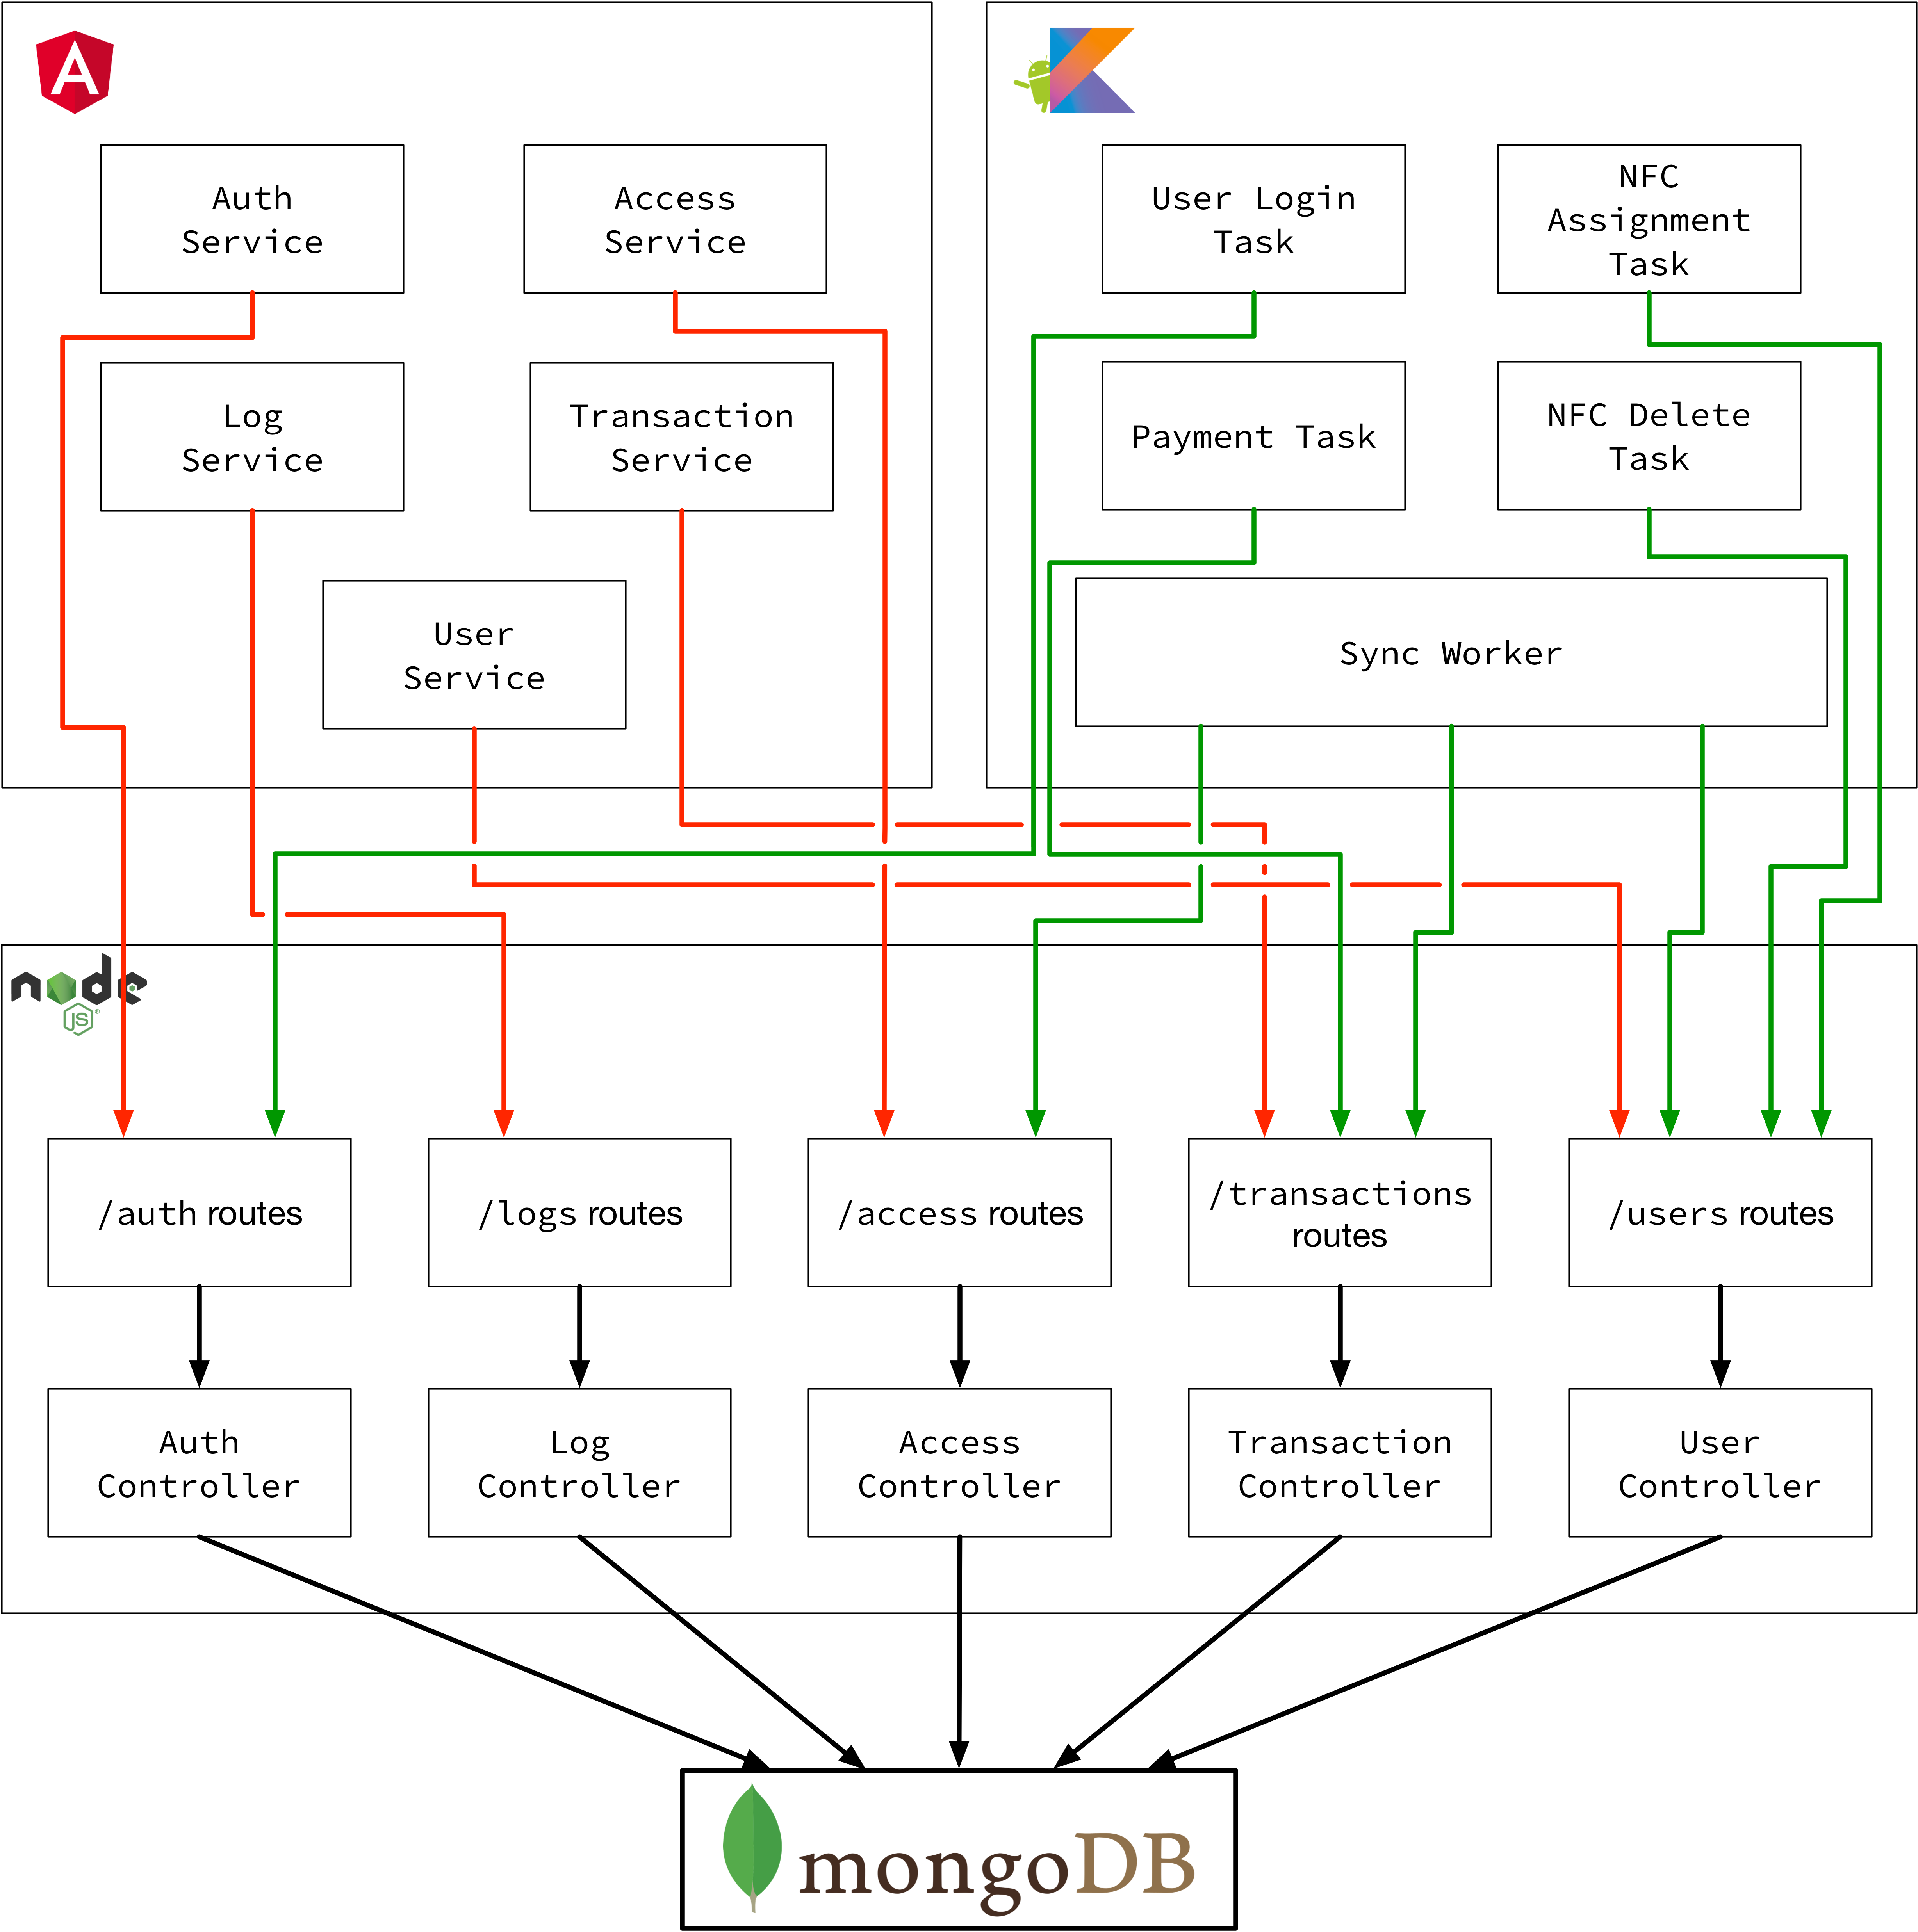
\includegraphics[width=\textwidth]{assets/implementation}
	\caption{Interactions between the components}
\end{center}
\end{figure}
%%TODO add explanation of figure
%%TODO add full architecture diagram of interaction between all technologies and modules
\section{Deployment}
\subsection{Deployment architecture}
\subsection{Nginx Proxy}
\section{Backend}
\subsection{Authentication}
\label{implementation_auth}
\subsection{Endpoints}
\subsection{Interaction with MongoDB}
\section{Angular frontend}
\begin{figure}[H]
\begin{center}
	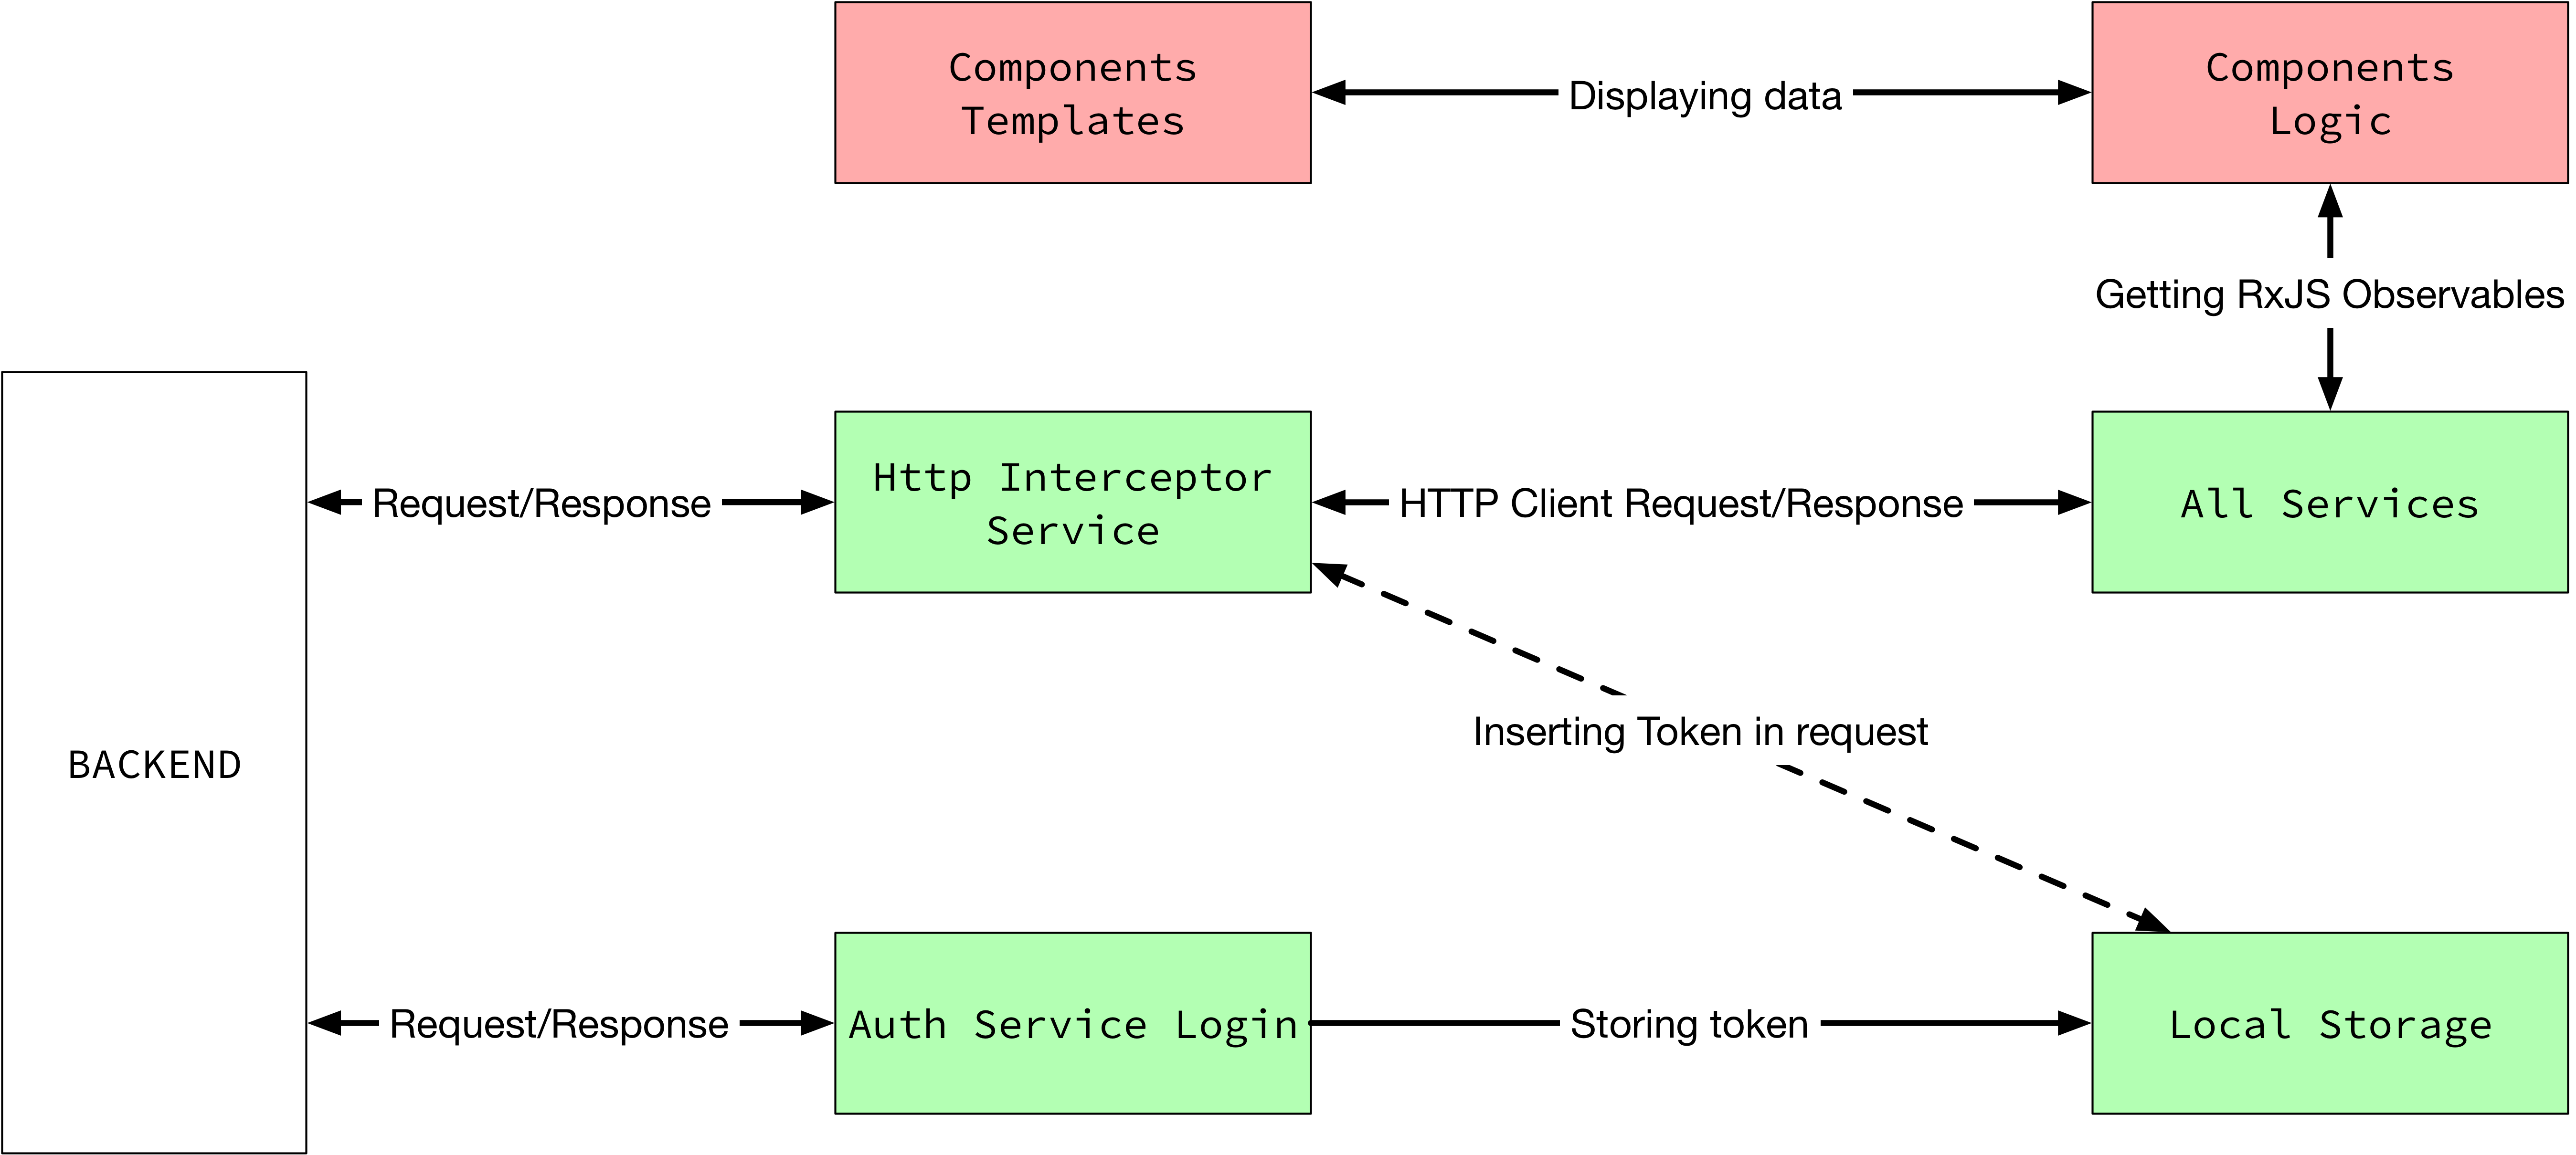
\includegraphics[width=\textwidth]{assets/angular_implementation}
	\caption[Interactions in the Angular Frontend]{Interactions in the Angular Frontend (Components in red, services in green)}
\end{center}
\end{figure}
\subsection{Authentication}
%%TODO http interceptor that adds JWT, JWT stored in LocalStorage
\subsection{Routing}
%%TODO insert nested routes variable
\subsection{Components}
\section{Android application}
\begin{figure}[H]
\begin{center}
	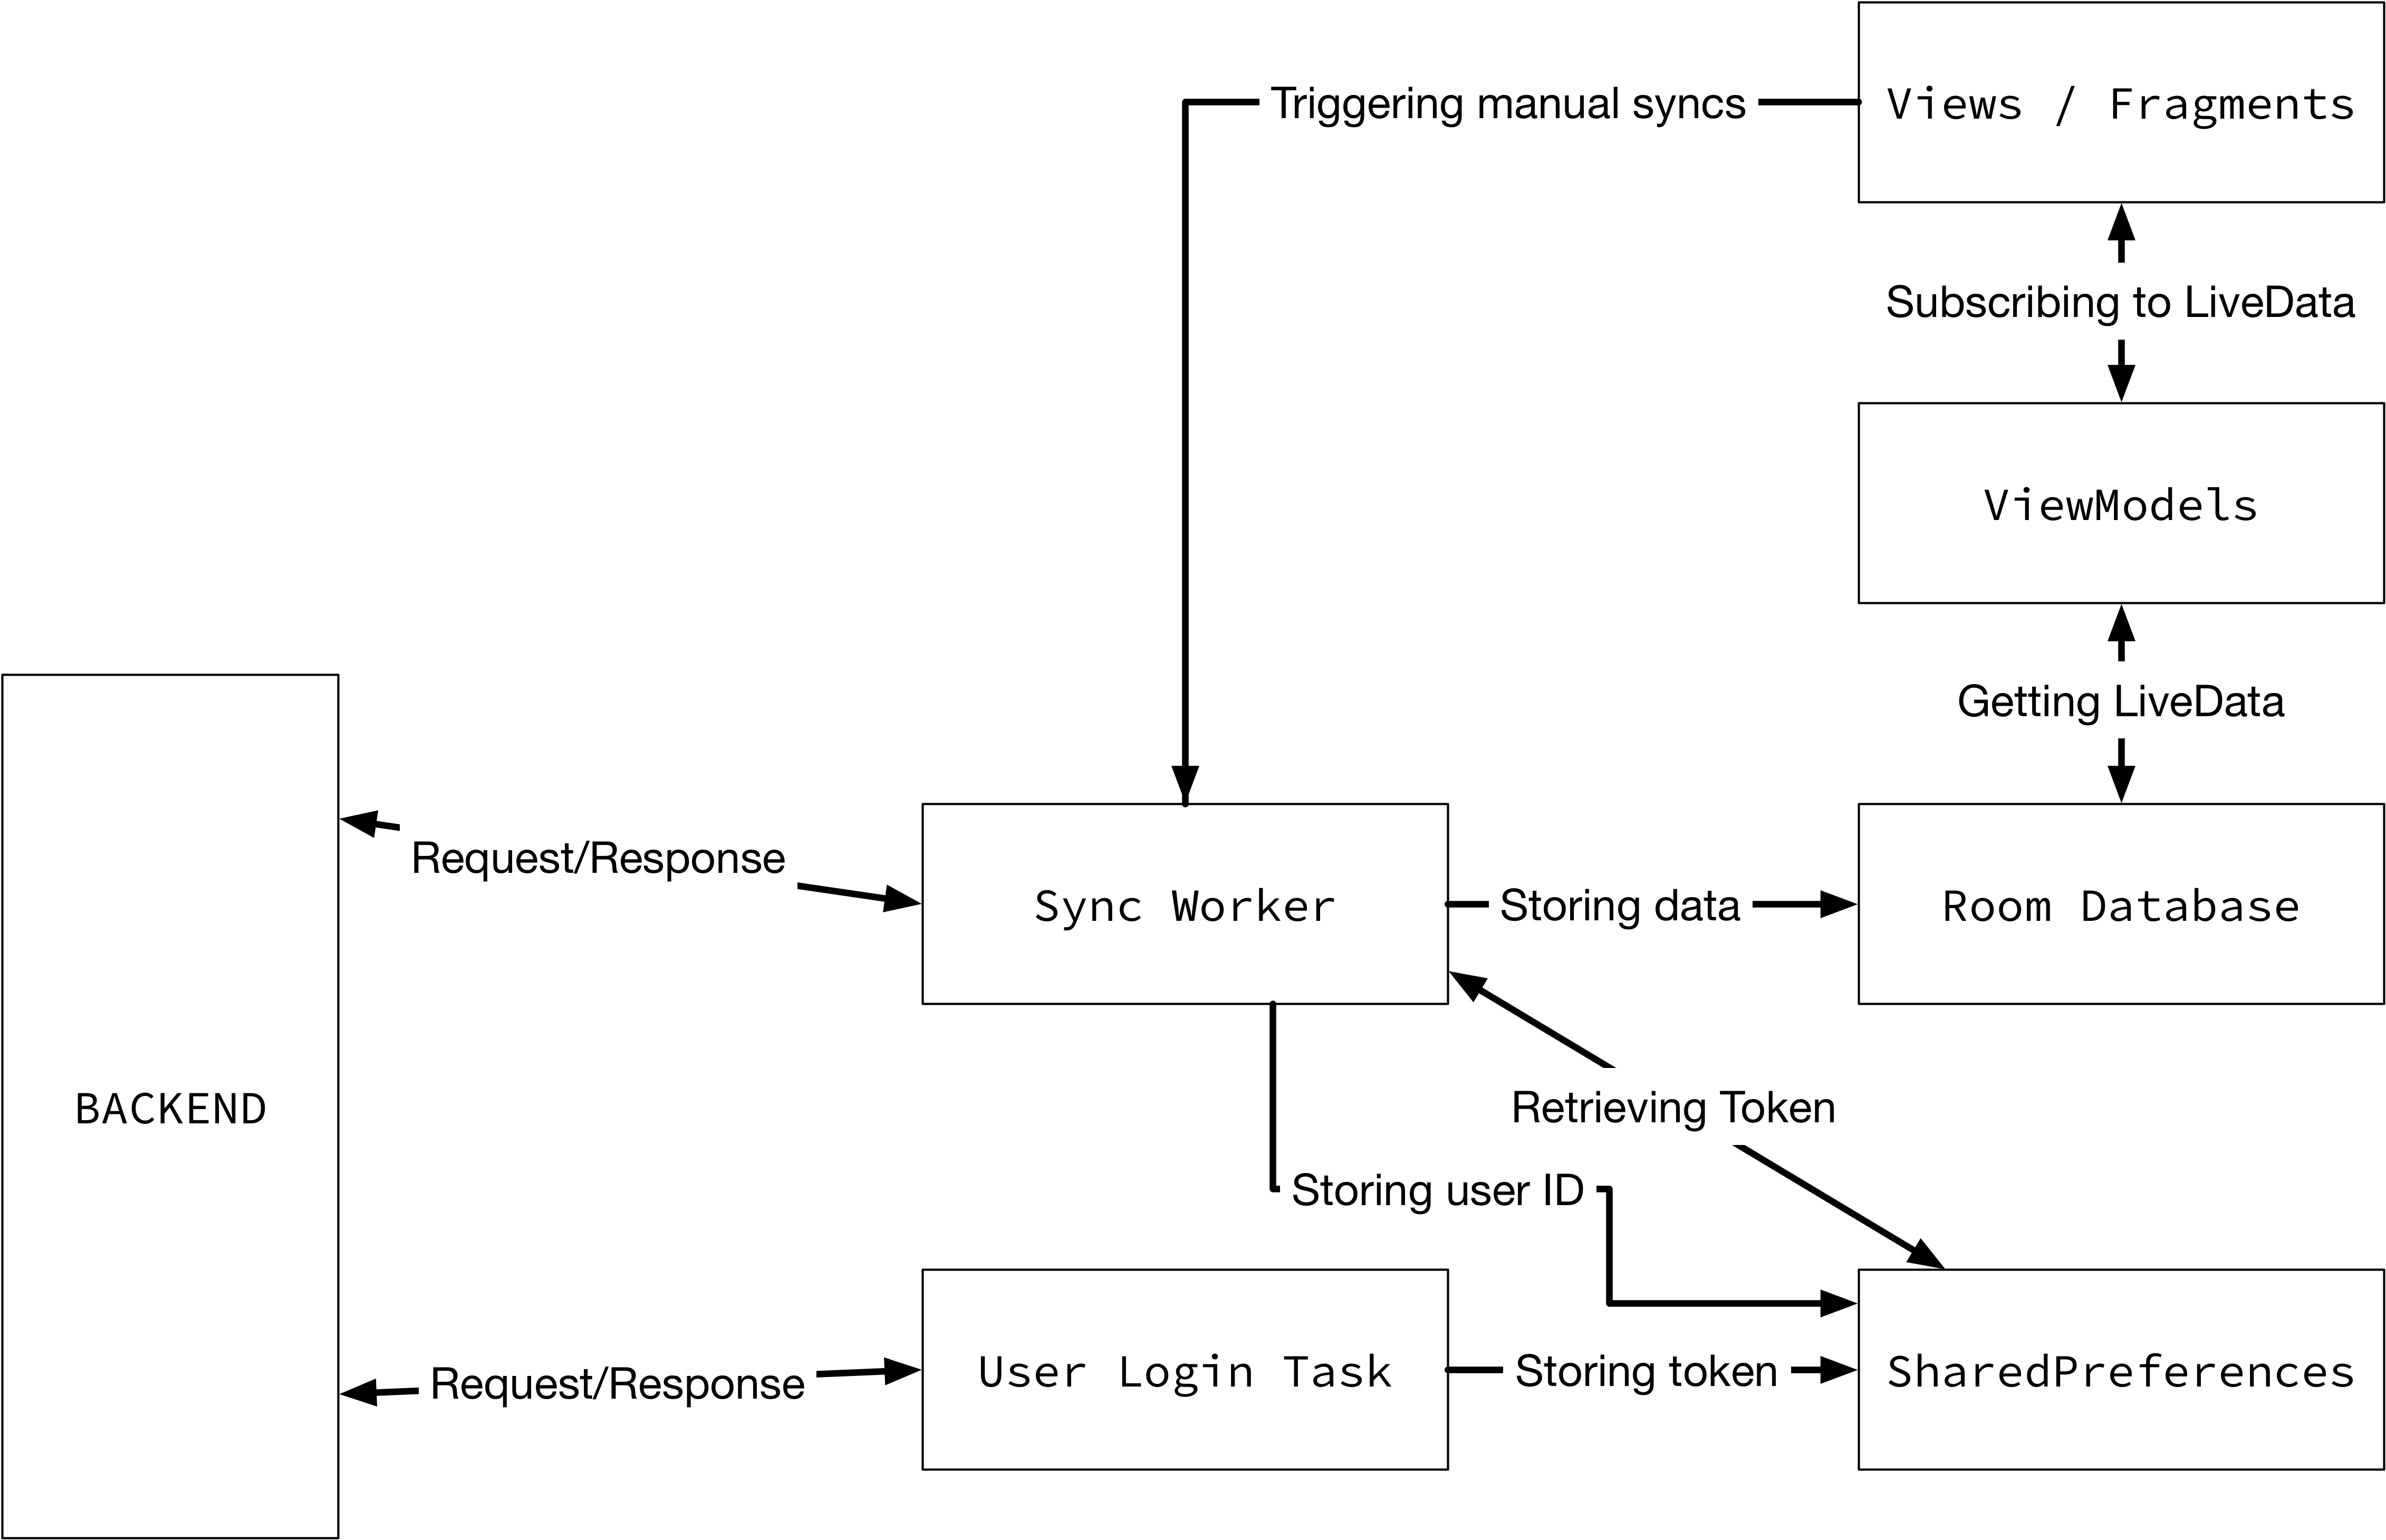
\includegraphics[width=\textwidth]{assets/android_implementation}
	\caption{Interactions in the Android application}
\end{center}
\end{figure}
\section{Deployment}
%%TODO REMOVE CONTAINER FROM TECHNOLOGIES AND PUT THEM ONLY IN DEPLOYMENT
%%TODO talk about basis linux container distribution
%%TODO talk about portability
\subsection{Docker}
\subsection{Orchestration with Docker Compose}
\subsection{Google Cloud}
\subsubsection{Kubernetes}
\subsubsection{Google Container Registry}
\subsection{Azure}
\chapter{Results}
\chapter{Conclusion}
%%TODO talk about how to implement new features or sections inside the project
\section{Future works}
\backmatter
\pagenumbering{Roman}
\pagestyle{plain}
\bibliographystyle{unsrt}
\bibliography{bibliography}
\begin{appendices}
\appendixpage
\chapter{Deployment guide}
%%TODO write deployment guide
\chapter{Backend API Documentation}
The documentation of the Backend \gls{api}, generated with APIDoc is available as an interactive version on \url{https://maximelovino.github.io/PocketHepia/api/}
\chapter{Android Documentation}
The documentation of the Android application, generated with Dokka is available as an interactive version on \url{https://maximelovino.github.io/PocketHepia/android/}
\end{appendices}



\end{document}
